\documentclass{scrartcl}[12pt, halfparskip]
\usepackage[utf8x]{inputenc}
\usepackage[T1]{fontenc}
\usepackage[english]{babel}
\usepackage{amsmath, amssymb, amstext}
\usepackage{wrapfig}
\usepackage{float}
\usepackage{graphicx}
\usepackage{color}
\usepackage{booktabs}
\usepackage{xfrac}
%\usepackage{amsthm}
\usepackage{ntheorem}
\usepackage{subcaption}
\usepackage{bbm}



\numberwithin{equation}{section}
\numberwithin{figure}{section}
\numberwithin{table}{section}

%\theoremstyle{break}
\newtheorem{Definition}{Definition}
\newtheorem{Theorem}{Theorem}
\newtheorem{Lemma}{Lemma}



\usepackage{pgfplots}
\usepackage{tikz}
\usetikzlibrary{fit} 
\usetikzlibrary{external}
%\tikzexternalize % activate!
%\usetikzlibrary{patterns}
\usetikzlibrary{patterns,decorations.pathreplacing}


    \tikzset{
    	hatch distance/.store in=\hatchdistance,
    	hatch distance=10pt,
    	hatch thickness/.store in=\hatchthickness,
    	hatch thickness=2pt
    }
    
    \makeatletter
    \pgfdeclarepatternformonly[\hatchdistance,\hatchthickness]{flexible hatch}
    {\pgfqpoint{0pt}{0pt}}
    {\pgfqpoint{\hatchdistance}{\hatchdistance}}
    {\pgfpoint{\hatchdistance-1pt}{\hatchdistance-1pt}}%
    {
    	\pgfsetcolor{\tikz@pattern@color}
    	\pgfsetlinewidth{\hatchthickness}
    	\pgfpathmoveto{\pgfqpoint{0pt}{0pt}}
    	\pgfpathlineto{\pgfqpoint{\hatchdistance}{\hatchdistance}}
    	\pgfusepath{stroke}
    }
    \makeatother



\newcommand\raalign[2]{%Umrahmen einer align-Gl.
	\tikz[overlay,every node/.style={inner sep=-2pt,outer sep=0pt}]%
	\node[anchor=base west](g){\phantom{$\displaystyle #1\null=\null#2$}}%
	node[draw=blue!50!black,fill=white!10,fit=(g),inner sep=5pt]{};%
	#1#2}


\usepackage{empheq}
\newcommand*\widefbox[1]{\fbox{\hspace{2em}#1\hspace{2em}}}


\usepackage{caption}
\usepackage{subcaption}

\bibliographystyle{unsrt}

\setlength{\parindent}{0pt}

\newcommand{\todo}[1]{\textcolor{red}{TODO: #1}}
\newcommand{\bem}[1]{\textcolor{blue}{Bem.: #1}}


\title{Master Thesis}


\author{Jan Lammel}
\date{\today{}, Heidelberg}



\begin{document}

\begin{titlepage}
	\begin{center}
	
	\textsc{\large Ruprecht-Karls-Universit\"{a}t Heidelberg} \\[0.5cm]
	\textsc{\large Master Thesis}\\[1cm]
	
	\newcommand{\HRule}{\rule{\linewidth}{0.5mm}}
	\HRule \\[0.4cm]
	\huge \bfseries Ueberschrift
	\HRule 
	
	\vspace{11cm}
	
	\Large \textit{Jan Lammel }\\
	\Large \textit{Heidelberg, \today }\\ \vspace{0.5cm}
	\Large \textit{Supervisor:}
	
	\Large \textit{Prof. Dr. Dr. h. c. mult. Hans Georg Bock}\\
	\Large \textit{Dr. Andreas Sommer}
	
	\end{center}
\end{titlepage}

\newpage

\tableofcontents 
\newpage

 \pagenumbering{Roman} 
 

 \addsec{Abstract}
 bla bla bla
 
 
 \newpage

\addsec{Zusammenfassung}
blubb !

\newpage
\pagenumbering{arabic}

\section{Introduction}
In this thesis we examine so called phase change materials (PCM). A popular application are heating pads (see Fig. \ref{fig:heating_pad}) which are liquid in a fully charged state. Folding induces a phase change to a solid state where energy is released and therefore the temperature increases. They can be easily recharged by applying a temperature above the melting point (e.g. with boiling water). 

\begin{wrapfigure}{l}{0.45\textwidth}
	\includegraphics[width=0.45\textwidth]{/home/argo/masterarbeit/thesis/images/handwaermer[wiki].jpg}
	\caption{Heating pad \\ left: liquid; right: solid}
	\label{fig:heating_pad}
\end{wrapfigure}

In general PCMs work as an energy buffer. Another application are industry processes to store the process heat for later usage \cite{pcm_process_heat}. Furthermore they can be used to optimize photovoltaic cells because their efficiency is temperature dependent and has a maximum at a certain point. PCMs are able to stabilize the temperature where the efficiency is maximal \cite{pcm_solar_cells}. 
As a last example we deal with insulations of houses. During the day when it is hot, the PCM becomes liquid and absorb heat from outside, so they work as a cooling system. On the contrary at night when it is cold outside the PCM becomes solid, releases heat and work as a heating \cite{pcm_house_insulation}. 


An important physical quantity is the specific heat capacity $c_p$ which tells us at which temperature the phase transition occurs and how much energy can be stored. The major goal of this thesis is to simulate the measuring process of a differential scanning calorimetry (DSC) where a PCM undergoes a phase transition and perform a parameter estimation in order to get the PCM's specific heat capacity. \\
As we will see in more detail in section \ref{sec:physics_DSC} the common way of computing $c_p(T)$ from DSC measurement data yields different results depending on the heat rate, a measurement parameter. Since $c_p(T)$ is a material property this is unphysical and this issue is known as the smearing problem. \\
By applying the parameter estimation we aim to avoid this problem. Furthermore the heat rate is proportional to the time duration of the experiment. If we get the same $c_p(T)$ for all heat rates we are able to accelerate the measuring process and therefore the research on this materials drastically. 
 


\section{Physical Background}
\subsection{Physical quantities and phase transition}

First of all some important physical quantities will be introduced because they are crucial for further comprehension. A summary is shown in Table \ref{tab:important_physical_quantities} with the consistently used symbol in this thesis and the physical unit. \\
Heat $Q$ is the energy that flows from a warmer to a colder object because of the temperature difference. The heat flux density $\phi$ tells us how much heat flows through an unit area in one second. It can be computed by Fourier's law: $\phi = - \lambda \nabla T$. By considering a particular area this changes to the heat flux $\varPhi$. Heat conductivity $\lambda$ is a material property how much energy is transported on a distance of $1m$, unit area and temperature difference of $1K$ in one second.

\begin{table}[H]
	\centering
\begin{tabular}{| c | c | c |} \hline
	Quantity & Symbol & Unit \\ \hline
	Heat & $Q$ & $J$ \\[0.7ex]
	Heat flux density & $\phi$ & $\frac{W}{m^2}$ \\[0.7ex]
	Heat flux & $\varPhi$ & $W$ \\[0.7ex]
	Heat conductivity & $\lambda$ & $\frac{W}{m \cdot K}$ \\[0.7ex]
	Specific heat capacity & $c_p$ & $\frac{J}{kg \cdot K}$ \\[0.7ex]
	Melting enthalpy & $\Delta H$ & $J$ \\ \hline
\end{tabular}
\caption{Important physical quantities}
\label{tab:important_physical_quantities}
\end{table}



Probably the most important physical quantity for us is the specific heat capacity $c_p$ which is a temperature dependent material property that tells us how much energy is needed to increase the temperature of $1kg$ of this material by $1K$. Since we are primarily interested in the phase change we handle with the so called apparent specific heat capacity which includes a peak at the melting point with a certain area equal to the melting enthalpy. For a pure substance this peak would be ideally a Dirac delta function (see Fig. \ref{fig:physics_c_p_dirac_delta}). A constant heat flux entering such a pure substance increases the temperature until phase change. Then the heat is absorbed in order to perform the phase transition while the temperature stays constant. Finally after the phase change has finished the temperature increases again. 
In mixed substances like PE in our case with different lengths of the individual polymer chains or due to lattice defects the peak extends over a temperature range. In the case of lattice defects the atom's binding energies are decreased which lowers the phase transition's temperature partially. The corresponding shape of the specific heat capacity is shown in Fig. \ref{fig:physics_fraser_suzuki} and is called Fraser-Suzuki peak. It is not known what shape of $c_p(T)$ we should expect exactly for a polymer and therefore task in this thesis to find out. \\
The last physical quantity to introduce is the melting enthalpy $\Delta H$ which is in the case of constant pressure the heat needed to perform the phase transition. Considering the graph $c_p(T)$, the area of the phase change peak is equal to the melting enthalpy. This is illustrated in Fig. \ref{fig:physics_fraser_suzuki}.



\begin{figure}[H]
\hspace{-2cm}
\begin{subfigure}{0.49\textwidth}
\begin{tikzpicture}
\begin{axis}[domain=70:150,
samples=500,
ymin=0, ymax=15	,	
xmin=70, xmax=150,	 
axis lines=left,
xtick=\empty,
ytick=\empty,
xlabel=$T$, xlabel style={at=(current axis.right of origin), anchor=west},
ylabel=\empty, ylabel style={at=(current axis.above origin), anchor=south}]

\addplot+[color=blue,
mark=none] {1.};
\addlegendentry{$c_p(T)$}

\draw[-latex,blue] (axis cs:130,1.) -- (axis cs:130,10);

\end{axis}
\end{tikzpicture}
\caption{}
\label{fig:physics_c_p_dirac_delta}
\end{subfigure}
\hspace{1.cm}
\begin{subfigure}{0.49\textwidth}
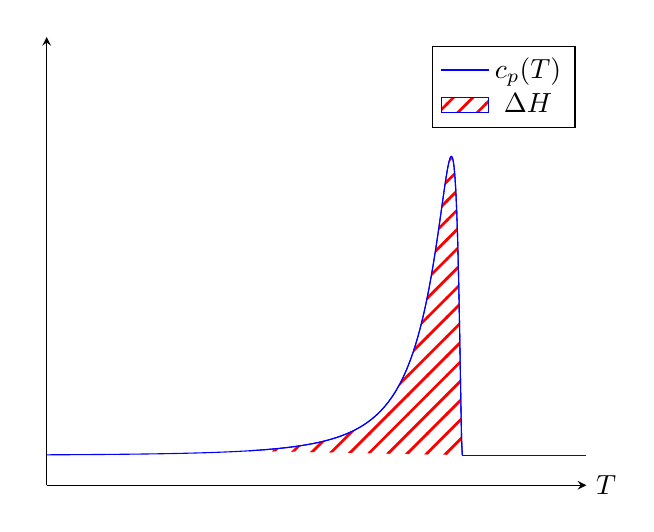
\begin{tikzpicture}
\begin{axis}[domain=70:132,
samples=500,
ymin=0, ymax=15	,	
xmin=70, xmax=150,	 
axis lines=left,
xtick=\empty,
ytick=\empty,
xlabel=$T$, xlabel style={at=(current axis.right of origin), anchor=west},
ylabel=\empty, ylabel style={at=(current axis.above origin), anchor=south}]

\addplot+[color=blue,
mark=none] {10*exp(-ln(2)/ln(0.3)^2 * (ln(1 + (x-130)*(0.3^2 - 1)/(5*0.3)))^2) + 1.};
\addlegendentry{$c_p(T)$}

\addplot+[mark=none,
color=blue,
domain=131.64:150,
samples=50,
forget plot]
{1.};

\addplot+[mark=none,
domain=100:132,
samples=500,
pattern=flexible hatch,
hatch distance=8pt,
hatch thickness=1pt,
draw=blue,
pattern color=red,
area legend]
{10*exp(-ln(2)/ln(0.3)^2 * (ln(1 + (x-130)*(0.3^2 - 1)/(5*0.3)))^2) + 1.};
\addlegendentry{$\Delta H$}
\end{axis}
\end{tikzpicture}
\caption{}
\label{fig:physics_fraser_suzuki}
\end{subfigure}
\caption{Specific heat capacity for (a) ideally pure substance where the phase transition is described by a Dirac delta function at the melting point and (b) mixed substance described by a Fraser-Suzuki Peak.}
\end{figure}



\subsection{Heat equation}
\label{sec:heat_equation}

Since we are dealing with heat transport in the measuring process the central equation in this thesis is the heat equation. \\
For the derivation \cite{lit:waerme_und_stoffuebertragung}
we start with the total inner energy $U$ in a volume $V$ which can be computed by

\begin{equation}
	U = \int_{V} \rho u \ dV
\end{equation}

where $\rho$ is the mass density and $u$ is the specific inner energy. \\
Next the total heat flux $\varPhi$ into the volume $V$ is

\begin{equation}
	\varPhi = - \int_{\partial V} \phi \cdot n \ dA = - \int_{V} \nabla \cdot \phi \ dV
\end{equation}

where $\phi$ is the heat flux density, $n$ is the normal vector pointing outside $dA$ (therefore the minus in front) and $\partial V$ is the surface of $V$. We have used Gauss theorem to transform the surface integral into a volume integral. \\
Now we assume that there are no further sources and sinks of inner energy for volume $V$ such that it holds

\begin{equation}
	\frac{\partial U}{\partial t} = \frac{\partial}{\partial t} \int_V (\rho u) \ dV = \int_V \frac{\partial}{\partial t}(\rho u) \ dV = - \int_{V} \nabla \cdot \phi \ dV = \varPhi
	\label{eq:heat_eq_derivation_1}
\end{equation}

for $\rho u$ continuous \todo{stimmt das?!}. The heat flux density is now computed with Fourier's law

\begin{equation}
	\phi = - \lambda \cdot \nabla T
	\label{eq:fouriers_law}
\end{equation}

with the heat conductivity $\lambda$. Since \eqref{eq:heat_eq_derivation_1} must hold for all volumes we can equate the integrands and insert \eqref{eq:fouriers_law} such that we get for a constant mass density $\rho$ and $u = u(T(x,t))$

\begin{align}
	\frac{\partial}{\partial t}(\rho u) = & \ \nabla \cdot \left[ \lambda \cdot \nabla T \right] \\
	\Leftrightarrow \ \ \rho \frac{\partial u}{\partial T} \frac{\partial T}{\partial t} = & \ \nabla \cdot \left[ \lambda \cdot \nabla T \right]
\end{align}

Due to the definition of the heat capacity $c_v(T) = \frac{\partial u}{\partial T}(T)$ and due to the assumption of a constant pressure $c_p = c_v$ we get the final heat equation

\begin{equation}
	\rho c_p(T) \frac{\partial T}{\partial t} = \nabla \cdot \left[ \lambda \cdot \nabla T \right]
	\label{eq:heat_equation_derivation}
\end{equation}




% ALT             
%
%\begin{equation}
%	\frac{\partial \rho_h}{\partial t} + \nabla \cdot J_q = 0
%\end{equation}
%
%where $\rho_h$ is the enthalpy density and $J_q$ is the heat flux density. We assume a constant pressure so it holds $dH = dQ$ such that a heat flux will only change the enthalpy.
%
%\begin{equation}
%	J_q = - \lambda \cdot \nabla T
%	\label{eq:fouriers_law}
%\end{equation}
%
%The enthalpy density $\rho_h = \rho h$ expressed with the mass density $\rho$ and specific enthalpy $h$ and Fourier's law inserted in the continuity equation gives us
%
%\begin{align}
%	\frac{\partial (\rho h)}{\partial t} = \nabla \cdot \left[\lambda \cdot \nabla T\right] \\
%	\Leftrightarrow \frac{\partial \rho}{\partial T} \frac{\partial T}{\partial t} h + \rho \frac{\partial h}{\partial T} \frac{\partial T}{\partial t} = \nabla \cdot \left[\lambda \cdot \nabla T\right] \\
%	\Leftrightarrow \left( \frac{\partial \rho}{\partial T} h + \rho \frac{\partial h}{\partial T} \right) \frac{\partial T}{\partial t} = \nabla \cdot \left[\lambda \cdot \nabla T\right]
%\end{align}
%
%Using the definition of the specific heat capacity $c_p := \frac{dh}{dT}$ we get the final heat equation
%
%\begin{equation}
%	\left( \frac{\partial \rho}{\partial T} h + \rho c_p \right) \frac{\partial T}{\partial t} = \nabla \cdot \left[\lambda \cdot \nabla T\right]
%\end{equation}
%
%\todo{Pruefen lassen ob das physikalisch alles so stimmt...}



\subsection{Differential Scanning Calorimetry}
\label{sec:physics_DSC}
The measuring method of a heat flux into a sample over a certain temperature range is called Differential Scanning Calorimetry (DSC). 

\begin{figure}[H]
	\centering
	\begin{subfigure}{0.49\textwidth}
		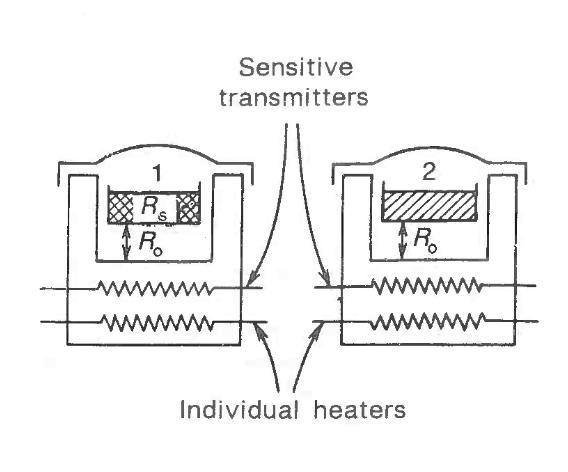
\includegraphics[width=1.\textwidth]{/home/argo/masterarbeit/thesis/images/dsc_principle.png}
		\caption{}
		\label{fig:DSC_power_compensated_principle}
	\end{subfigure}
	\begin{subfigure}{0.49\textwidth}
		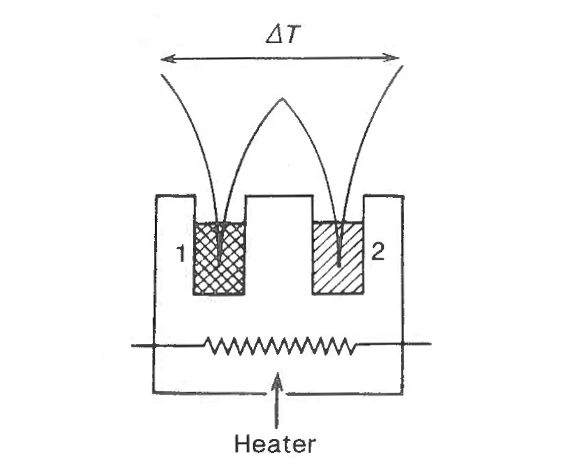
\includegraphics[width=1.\textwidth]{/home/argo/masterarbeit/thesis/images/dta_principle.png}
		\caption{}
		\label{fig:DTA_principle}
	\end{subfigure}
	\caption{Principal experimental setup of (a) power compensated DSC and \\ (b) DTA \cite{DSC_buch}.}
\end{figure}


\subsubsection{Power compensated DSC}
In the case of a power compensated DSC (Fig. \ref{fig:DSC_power_compensated_principle}) there are 2 seperated chambers for a reference and the sample. Both have individual heaters and temperature sensors such that a feedback control system keep the temperature in both chambers on the same value. Since we know the electrical power for heating we get the heat flux due to energy conservation. \\



\subsubsection{Heat flux DSC}
The heat flux DSC is based on differential thermal analysis (DTA, see Fig. \ref{fig:DTA_principle}). 
In DTA there is just one chamber in which both reference and sample are heated equally. 
Due to differences in the heat capacity of reference and sample a temperature difference dependent on their temperature will appear.
This can be used to find typical temperatures of known substances to identify the sample's components. \\
Unfortunately calorimetric properties like melting enthalpy are not accessible just from the temperature difference measurement. 
Note that the physical quantity measured is an electrical potential difference $\Delta U$ which is assumed to be proportional to the temperature difference due to the Seebeck effect. \\

\begin{figure}[H]
	\centering
	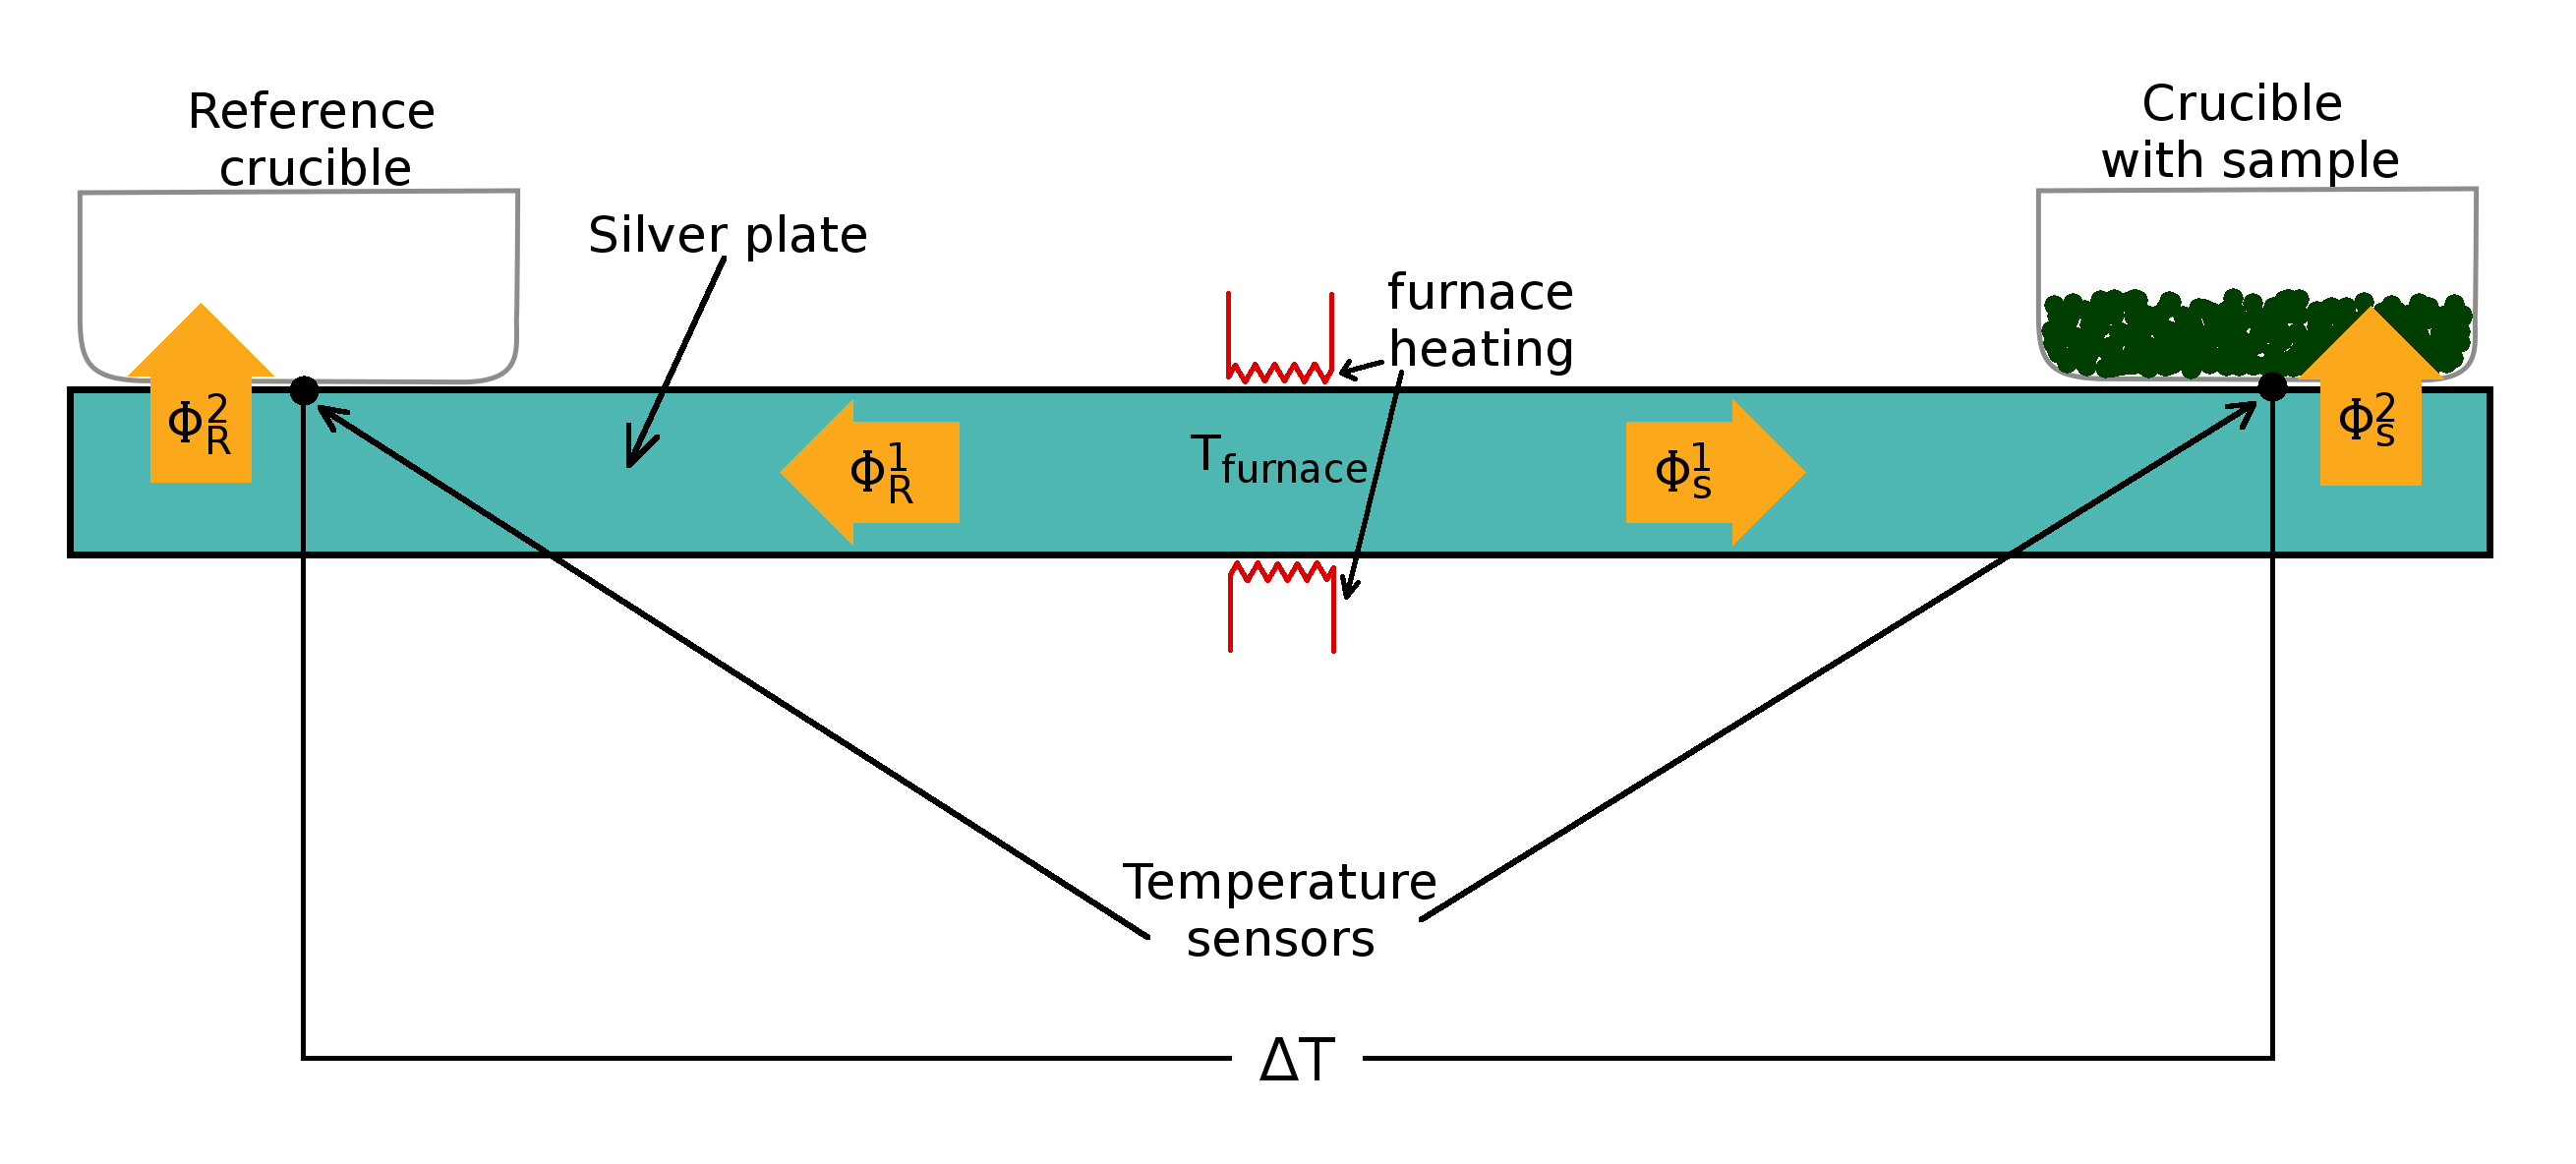
\includegraphics[width=1.\textwidth]{/home/argo/masterarbeit/vortrag/images/dsc_funktionsprinzip.png}
	\caption{Principle experimental scheme of DSC which has been used for measurements. Two crucibles (an empty reference one and the other filled with the sample to examine) are connected to the furnace with a silver plate. The furnace' temperature increases with time and because of thermal differences a temperature difference $\Delta T$ is measured with temperature sensors placed at the crucibles. The final measurement quantity we obtain by calibration is the heat flux into the sample $\varPhi_s^2$.}
	\label{fig:heat_flux_DSC}
\end{figure}

The heat flux DSC (see Fig. \ref{fig:heat_flux_DSC}) extends now DTA by computing the heat flux into the sample $\Phi_S^2$ from the temperature difference using an additional calibration. 
Pure materials with known melting temperature $T_{\text{Kal}}$ and melting heat $\Delta Q_{\text{Kal}}$ are measured, giving the measuring signal $\Delta U(t)$ with a peak at the phase change. 
The area of this peak is assumed to be proportional with constant $sens$ called sensitivity to the melting heat due to

\begin{equation}
	A_{\Delta U} \propto \Delta Q_{\text{Kal}} \quad \Rightarrow \quad sens = \frac{A_{\Delta U}}{\Delta Q_{\text{Kal}}}
\end{equation} 

This is done for a set of calibration materials such that we get a mapping $sens(T)$ by interpolating the data points $(T_{\text{Kal,i}}, sens_i)$, see Fig. \ref{fig:dsc-calibration_sens(T)}.

\begin{figure}[H]
	\centering
	\begin{subfigure}{0.45\textwidth}
		\centering
		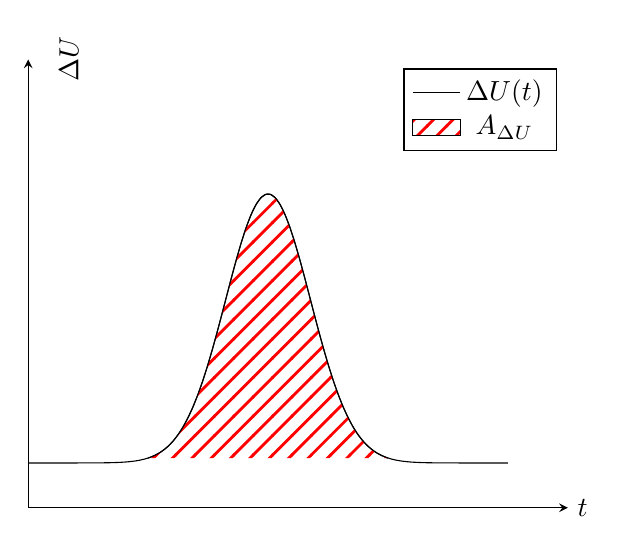
\begin{tikzpicture}
		\begin{axis}[domain=-1:7,
		samples=100,
		ymin=0, ymax=5	,	
		xmin=-1, xmax=8,	 
		axis lines=left,
		xtick=\empty,
		ytick=\empty,
		xlabel=$t$, xlabel style={at=(current axis.right of origin), anchor=west},
		ylabel=$\Delta U$, ylabel style={at=(current axis.above origin), anchor=south}]
		
		\addplot+[color=black,
		mark=none] {3*exp(-(x-3)^2) + 0.5};
		\addlegendentry{$\Delta U(t)$}
		\addplot+[mark=none,
		domain=1:5,
		samples=100,
		pattern=flexible hatch,
		hatch distance=8pt,
		hatch thickness=1pt,
		draw=black,
		pattern color=red,
		area legend]
		{3*exp(-(x-3)^2) + 0.5};
		\addlegendentry{$A_{\Delta U}$}
		\end{axis}
		\end{tikzpicture}
		\caption{}
		\label{fig:dsc-calibration_dU(t)}
	\end{subfigure}
	\hfill
	\begin{subfigure}{0.45\textwidth}
		\begin{tikzpicture}
		\begin{axis}[domain=-1:6.3,
		samples=100,
		ymin=0, ymax=5	,	
		xmin=-1, xmax=8,	 
		axis lines=left,
		xtick={2, 4},
		xticklabels={$T_{Kal,i}$, $T_{Kal,i+1}$},
		ytick=\empty,
		xlabel=$T$, xlabel style={at=(current axis.right of origin), anchor=west},
		ylabel=$sens$, ylabel style={at=(current axis.above origin), anchor=south}
		]
		
		\addplot+[color=black, mark=none] {3 - 0.1*x - 0.005*x^2};
		\addplot[only marks, mark=x, color=black] 
		table {0 3.
			1 2.9
			2 2.8
			4 2.55
			5 2.4
		};
		\end{axis}
		\end{tikzpicture}
		\caption{}
		\label{fig:dsc-calibration_sens(T)}
	\end{subfigure}
	\caption{Sensitivity calibration graphs: (a) Computing for a material with known melting point $T_{\text{Kal}}$ and enthalpy $\Delta Q_{\text{Kal}}$ the area $A_{\Delta U}$ under the measuring signal $\Delta U(t)$ graph which is related to melting enthalpy via factor $sens$. Perform this for several materials such that in (b) we can interpolate $sens=\frac{A_{\Delta U}}{\Delta Q_{\text{Kal}}}$ for a certain temperature range.}
\end{figure}

With the mapping $\Phi(T_{ref}) = \frac{\Delta U(T_{ref})}{sens(T_{ref})}$ the heat flux into the sample then can be computed for a measurement signal $\Delta U$ of unknown materials. 




\subsubsection{Smearing Problem}
\label{sec:smearing_problem}
The common way to perform the DSC calibration, measurement and compute the specific heat capacity $c_p$ is described in detail in DIN 11357 \cite{DIN_11357}. By assuming a proportionality between the heat flux into the sample and the sample's heat capacity one gets the equation

\begin{equation}
	c_p^S(T) = c_p^{R}(T) \cdot \frac{m^R}{m^S} \cdot \frac{\Phi^S(T) - \Phi^0(T)}{\Phi^R(T) - \Phi^0(T)}
	\label{eq:c_p_formula_DIN}
\end{equation}

where $S$ and $R$ denote the sample respectively reference. Reference means here a material with known specific heat capacity $c_p^R(T)$, not to be mistaken with the reference side of the experimental setup. In our case this reference material is Saphir. $m$ is the mass and $\Phi^0$ is the heat flux if both crucibles are empty to compensate asymmetries. \\
In Fig. \ref{fig:heat_flux_measurements} the measurement data of the heat flux into the PCM is shown for all heat rates dependent on the temperature at the reference crucible. Using \eqref{eq:c_p_formula_DIN} the computed specific heat capacities for the PCM are shown in Fig. \ref{fig:c_p_DIN_formula}. As one can see for higher heat rates the peak position shifts to higher temperatures and furthermore the peak is smeared out. This is known as the smearing problem since $c_p$ is a material property and must be equal for all heat rates.


\begin{figure}[H]
	\centering
	\begin{subfigure}{0.7\textwidth}
		\includegraphics[width=1.\textwidth]{/home/argo/masterarbeit/thesis/images/heat_flux_measurement.png}
		\caption{}
		\label{fig:heat_flux_measurements}
	\end{subfigure}
	\begin{subfigure}{0.7\textwidth}
		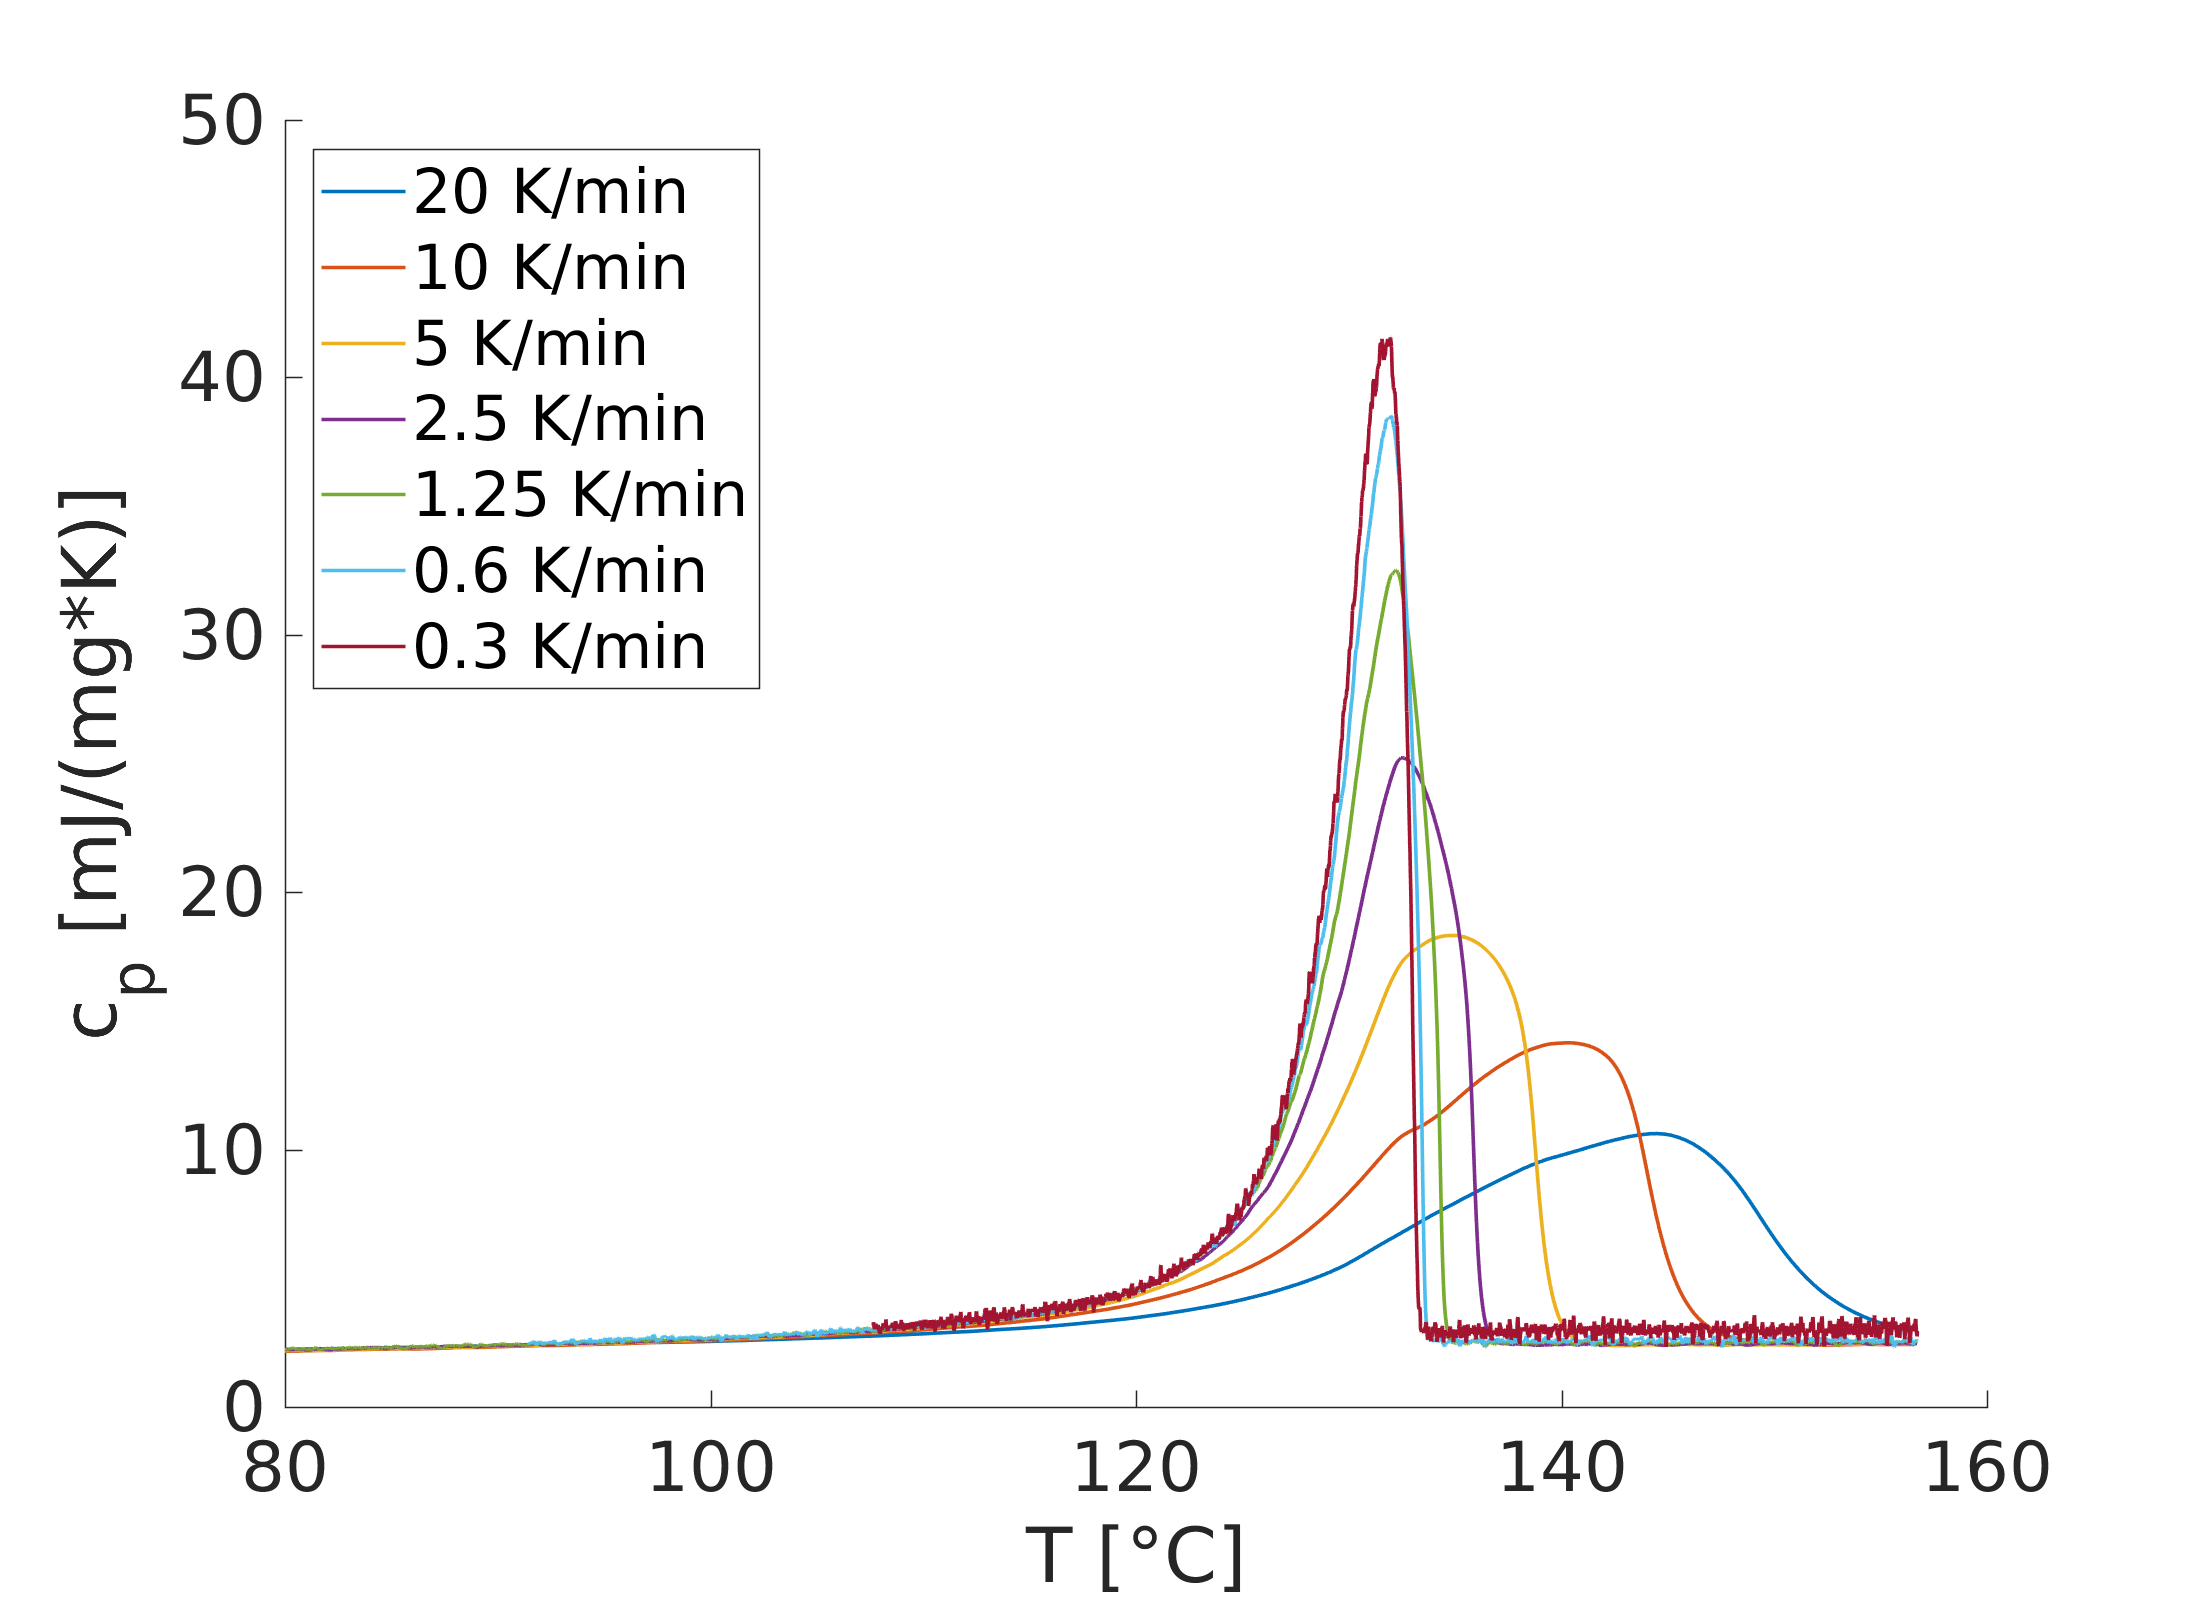
\includegraphics[width=1.\textwidth]{/home/argo/masterarbeit/thesis/images/c_p_DIN_formula.png}
		\caption{}
		\label{fig:c_p_DIN_formula}
	\end{subfigure}
	\caption{(a) Heat flux measurement values $\eta^{\varPhi}(T_{ref})$ and (b) computed $c_p(T)$ using eq. \eqref{eq:c_p_formula_DIN} with distinctly and visible smearing effect for higher heat rates.}
\end{figure}


\newpage
\section{Mathematical Background}

\subsection{Derivative generation}
In the context of continuous optimization we are dependent on derivative information in order to minimize some function. 
There are several possibilities to obtain these derivatives. We will introduce here the concept of finite differences and automatic differentiation which were used in this thesis. 
Beside them the methods of symbolic- and complex step-differentiation exist and are explained in detail in \cite{diss_jan}.

\subsubsection{Finite Differences}
\label{subsubsec:finite_differences}
Derivatives generated by finite differences are needed beside the optimization task also in the spatial discretization of a partial differential equation which will be explained in more detail in section \ref{subsection:pde_discretization}.
They can be derived easily from Taylor-series expansion. Considering the function $f: \mathcal{R} \rightarrow \mathcal{R}^m$ the Taylor series looks as follows:


\begin{equation}
f(x+h) = f(x) + h \cdot \frac{\partial f}{\partial x}(x) + \mathcal{O}(h^2)
\end{equation}

Reordering gives the one-sided derivative approximation

\begin{equation}
\frac{\partial f}{\partial x}(x) = \frac{f(x+h) - f(x)}{h} + \mathcal{O}(h^2)
\end{equation}

Regarding the Taylor series up to order two in both directions of the domain of definition,

\begin{subequations}
	\label{eq:finite_differences_taylor_exp}
	\begin{align}
	f(x+h) = f(x) + h \cdot \frac{\partial f}{\partial x}(x) + \frac{h^2}{2} \cdot \frac{\partial^2 f}{\partial^2 x}(x) + \mathcal{O}(h^3) \label{eq:finite_differences_taylor_exp_+} \\
	f(x-h) = f(x) - h \cdot \frac{\partial f}{\partial x}(x) + \frac{h^2}{2} \cdot \frac{\partial^2 f}{\partial^2 x}(x) + \mathcal{O}(h^3)  \label{eq:finite_differences_taylor_exp_-}	
	\end{align}
\end{subequations}


subtract both equations and reorder again we get

\begin{equation}
\frac{\partial f}{\partial x}(x) = \frac{f(x+h) - f(x-h)}{2 h} + \mathcal{O}(h^3)
\end{equation}

which has a higher error order but at the expense of two function evaluations. \\

Second order derivatives can be gained analogously by adding \eqref{eq:finite_differences_taylor_exp_+} and \eqref{eq:finite_differences_taylor_exp_-}:

\begin{equation}
\frac{\partial^2 f}{\partial^2 x}(x) = \frac{f(x-h) - 2 \cdot f(x) + f(x+h)}{h^2} + \mathcal{O}(h^3)
\label{eq:finite_difference_2nd_der}
\end{equation}





In the spatial discretization of partial differential equations one often choose a finer grid for areas of interest. So for the resulting non-equidistant grid (see Fig. \ref{fig:2_point_formula_illustration}) one needs a more general formula which is derived by considering again the Taylor expansion





\begin{subequations}
	\label{eq:finite_differences_taylor_exp_non-homogenous}
	\begin{align}
	f(x-h) = & f(x) - h \cdot \frac{\partial f}{\partial x}(x) + \frac{h^2}{2} \cdot \frac{\partial^2 f}{\partial^2 x}(x) + \mathcal{O}(h^3) \label{eq:finite_differences_taylor_exp_non-homogenous_1} \\
	f(x+\alpha h) = & f(x) + \alpha h \cdot \frac{\partial f}{\partial x}(x) + \frac{\alpha^2 h^2}{2} \cdot \frac{\partial^2 f}{\partial^2 x}(x) + \mathcal{O}(h^3)  \label{eq:finite_differences_taylor_exp_non-homogenous_2}
	\end{align}
\end{subequations}



Multiplying \eqref{eq:finite_differences_taylor_exp_non-homogenous_1} with $\alpha$ and adding \eqref{eq:finite_differences_taylor_exp_non-homogenous_2} gives

\begin{align}
\alpha f(x-h) + f(x+\alpha h) = \alpha f(x) + \alpha \frac{h^2}{2} \frac{\partial^2 f}{\partial^2 x}(x) + f(x) + \frac{\alpha^2 h^2}{2} \frac{\partial^2 f}{\partial^2 x}(x) + \mathcal{O}(h^3)  \\
\Leftrightarrow (\alpha+1) \frac{\alpha h^2}{2} \frac{\partial^2 f}{\partial^2 x}(x) = \alpha f(x-h) - (\alpha+1) f(x) + f(x+\alpha h) + \mathcal{O}(h^3) 
\end{align}

\begin{equation}
\Leftrightarrow \frac{\partial^2 f}{\partial^2 x}(x) = \frac{1}{h^2} \left[ \frac{2}{1+\alpha} f(x-h) - \frac{2}{\alpha} f(x) + \frac{2}{\alpha (\alpha+1)} f(x+\alpha h) \right] + \mathcal{O}(h^3) 
\label{eq:2_point_formula_inhomogeneous}
\end{equation} \\

Note that for a homogeneous grid ($\alpha=1$) this is obviously equal to \eqref{eq:finite_difference_2nd_der}. \\

\begin{figure}[H]
	\centering
	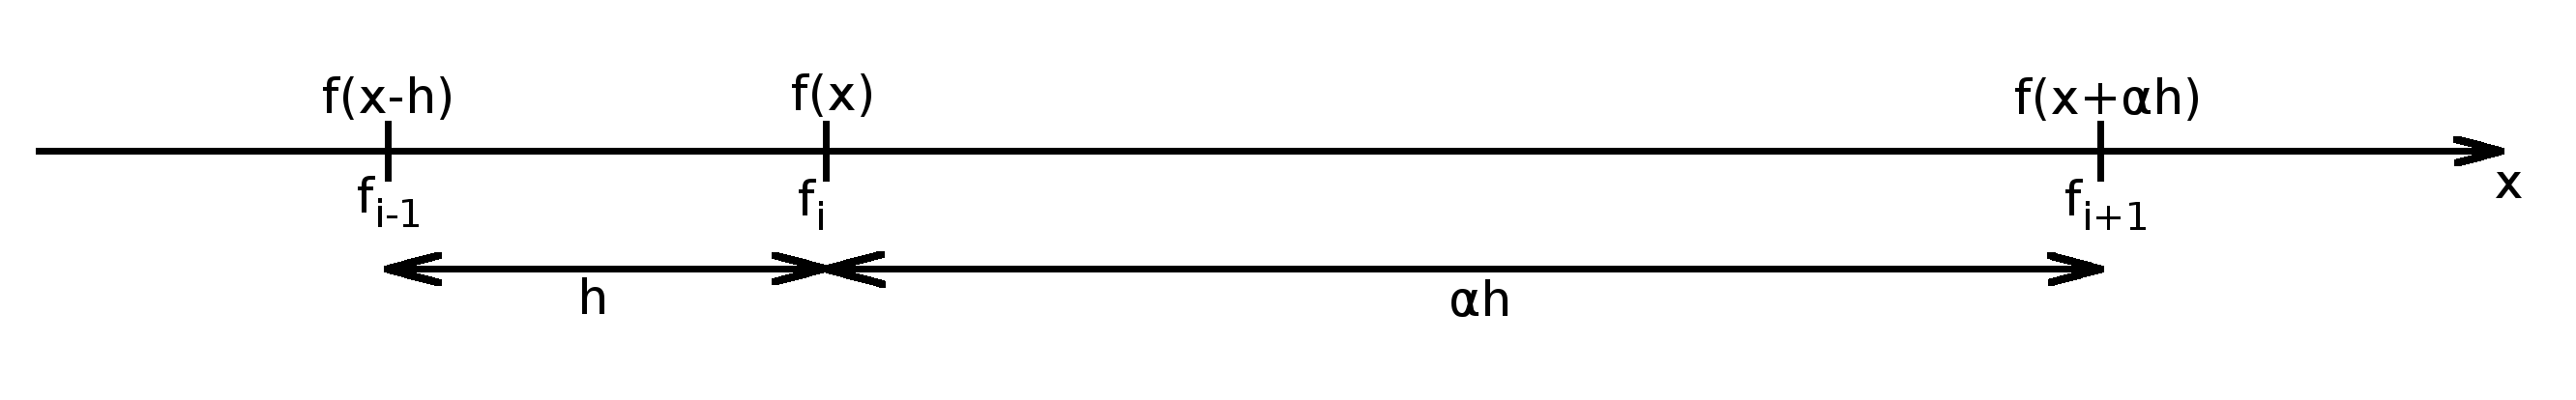
\includegraphics[width=1.\textwidth]{/home/argo/masterarbeit/thesis/images/2nd_derivative_2-point_formula_illustration.png}
	\caption{Function $f(x)$ and its discretization $f_i$ on a non-equidistant grid.}
	\label{fig:2_point_formula_illustration}
\end{figure}


For simplicity we restricted the function argument $x \in \mathcal{R}$. In the case $x \in \mathcal{R}^n$ the Jacobian is gained by performing directional derivatives. So e.g. for the one-sided first derivative $n+1$ function evaluations are necessary. \\

The great advantage of finite differences are their simple implementation. We can treat the (arbitrarily elaborate) function as a black box, perturb the input arguments a bit, perform $n+1$ function evaluations and get an approximation of the derivative. \\
This simplicity is at the expense of accuracy. If we choose $h$ too small, cancellation occurs. Otherwise with $h$ large the remainder term of the Taylor expansion gets large as well. So there exist an optimal $h$ to minimize the error although then the derivative approximation is still not exact.




\subsubsection{Automatic Differentiation and Internal Numerical Differentiation}
The basic idea of Automatic Differentiation (AD) is to subdivide a function $f: \mathcal{R}^n \rightarrow \mathcal{R}^m$ into so called elementary functions $\varphi_i$ from which the derivative is known. 

The evaluation of these elementary functions give intermediate values $v_i = \varphi(v_j)_{j \prec i}$ where the dependency relation $\prec$ is defined as

\begin{equation}
j \prec i \Leftrightarrow v_j \text{\textit{ is an argument of }} \varphi_i.
\end{equation}

By successively applying the chain rule one obtains the derivative of $f$.
One can distinguish the forward and reverse mode which will be explained in more detail now and exemplified by means of the example function

\begin{equation}
F(x) = 
\begin{bmatrix}
\exp((1+x_1)^2) + x_3 \\
x_2 \cdot \sin(1+x_1)
\end{bmatrix}
\end{equation}


\paragraph{Forward Mode}\mbox{}\\
In the forward mode the directional derivative $\dot{y}$ is computed for a given direction in the function arguments $\dot{x}$ at a evaluation point $x$:

\begin{equation}
\dot{y} = \frac{\partial f}{\partial x}(x) \cdot \dot{x}
\label{eq:AD_example}
\end{equation}

The algorithm called first order forward sweep is structured into three parts. First the auxiliary variables $v_{1-n},...,v_0$ and $\dot{v}_{1-n},...,\dot{v}_0$ are initialized with the evaluation point $x$ and the direction of the directional derivative $\dot{x}$. So if we want to get $\frac{\partial f}{\partial x_2}$ we would need to set $\dot{x} = \begin{bmatrix}
0 & 1 & 0 & \dots & 0
\end{bmatrix}^T$. One can see here that with one forward sweep we get one column of the Jacobian $ \frac{\partial f}{\partial x}$. 
After the initialization the actual forward sweep begins where the $k$ elemental functions of $f$ are evaluated and saved in the intermediate values $v_i$. Simultaneously their derivatives  $\dot{v}_i$ are computed using previously calculated intermediate values. E.g. for $v_2 = \varphi_2(v_0, v_1)$ it holds $\dot{v}_2 = \frac{\partial \varphi_2}{\partial v_0} \dot{v_0} + \frac{\partial \varphi_2}{\partial v_1} \dot{v_1}$. \\
The last $m$ intermediate variables represent the solution vector. So finally this values and derivatives are extracted.



\begin{table}[H]
	\begin{tabular}{|c | l c l | l |} \hline
		Initialization & $[v_{i-n}, \dot{v}_{i-n}]$ & $=$ & $[x_i, \dot{x}_i]$ & $i=1,...,n$ \\ \hline
		Intermediate steps & $[v_{i}, \dot{v}_{i}]$ & $=$ & $[\varphi_i(v_j)_{j \prec i}, \sum_{j \prec i} \frac{\partial \varphi_i}{\partial v_j}(v_j) \cdot \dot{v}_j]$ & $i=1,...,k$ \\ \hline
		Extract solution & $[y_{m-i}, \dot{y}_{m-i}]$ & $=$ & $[v_{k-i}, \dot{v}_{k-i}]$ & $i=m-1,...,0$ \\ \hline
	\end{tabular}
	\caption{First order forward sweep}
	\label{tab:first_order_forward_sweep}
\end{table}

In order to illustrate this algorithm we will apply it on the example function \eqref{eq:AD_example}:

\begin{table}[H]
	\centering
	\begin{tabular}{| c | l | l |} \hline
		Initialization & $v_{-2} = x_1$ & $\dot{v}_{-2} = \dot{x_1}$ \\
		& $v_{-1} = x_2$ & $\dot{v}_{-1} = \dot{x}_2$ \\
		& $v_{0} = x_3$ & $\dot{v_{0}} = \dot{x}_3$ \\ \hline
		Intermediate Steps & $v_1 = 1+v_{-2}$ & $\dot{v_1} = 1 \cdot \dot{v}_{-2}$ \\
		& $v_2 = v_{1}^2$ & $\dot{v_2} = 2 v_1 \cdot \dot{v}_{1}$ \\
		& $v_3 = \exp(v_{2})$ & $\dot{v_3} = \exp(v_2) \cdot \dot{v}_{2}$ \\
		& $v_4 = \sin(v_{1})$ & $\dot{v_4} = \cos(v_1) \cdot \dot{v}_{1}$ \\
		& $v_{5} = v_3 + v_0$ & $\dot{v_{5}} = 1 \cdot \dot{v}_3 + 1 \cdot \dot{v}_0$ \\
		& $v_{6} = v_{-1} + v_4$ & $\dot{v_{6}} = v_4 \cdot \dot{v}_{-1} + v_4 \cdot \dot{v}_{-1}$ \\ \hline
		Extract  solution & $y_1 = v_5$ & $\dot{y}_1 = \dot{v}_5$ \\
		& $y_2 = v_6$ & $\dot{y}_2 = \dot{v}_6$ \\ \hline
	\end{tabular}
	\caption{First order forward sweep applied on \eqref{eq:AD_example}.}
\end{table}




\paragraph{Adjoint Mode}\mbox{}\\
Beside the forward mode there is the adjoint mode where the adjoint directional derivative $\bar{x}^T$ is computed for a given adjoint direction $\bar{y}^T$ at the evaluation point $x$. 

\begin{equation}
\bar{x}^T = \bar{y}^T \frac{\partial f}{\partial x}(x)
\end{equation}

The algorithm is shown in Table \ref{tab:first_order_adjoint_sweep}. In contrary to the forward mode we need here an additional set of adjoint intermediate variables $\bar{v}_i$. These contain the adjoint sensitivity information which are initialized to zero in the first step. \\
The following forward sweep is analog to the one shown in Table \ref{tab:first_order_forward_sweep}, however here we compute just the intermediate function evaluations without derivatives. We need these function values in the next part. \\
The actual adjoint directional derivatives are now computed in the reverse sweep which consists of three sub-steps. First of all the adjoint directions $\bar{y}$ is chosen. So for example, if we want the second row of the Jacobian $\frac{\partial f_2}{\partial x}$ we need to set $\bar{y} = \begin{bmatrix}
0 & 1 & 0 & \dots & 0
\end{bmatrix}^T$.
Next all contributions to the adjoint intermediate variables will be successively summed up by applying the adjoint equation $\bar{y}^T \dot{y} = \bar{y}^T J \dot{x} = \bar{x}^T \dot{x}$ in a reverse scheme (that is why we need the forward sweep and hence the intermediate value evaluations first). Finally we can extract the solution $\bar{x}$ which corresponds to a row in $\frac{\partial f}{\partial x}$.


\begin{table}[H]
	\centering
	\begin{tabular}{| c | l c l | l |} \hline
		Initialization & $\bar{v}_i$ & $=$ & $0$ & $i=1-n,...,k-m$ \\ \hline
		& $v_{i-n}$ & $=$ & $x_i$ & $i=1,...,n$ \\
		Forward Sweep & $v_{i}$ & $=$ & $\varphi_i(v_j)_{j \prec i}$ & $i=1,...,k$ \\
		& $y_{m-i}$ & $=$ & $v_{k-i}$ & $i=m-1,...,0$ \\ \hline
		& $\bar{v}_{k-i}$ & $=$ & $\bar{y}_{m-i}$ & $i=0,...,m-1$ \\
		Reverse Sweep & $\bar{v}_j$ & $+ \hspace{-0.1cm} =$ & $\bar{v}_i \frac{\partial \varphi_i}{\partial v_j}(v_j) \quad \forall \ j \prec i$ & $i=k,...,1$ \\
		& $\bar{x}_i$ & $=$ & $\bar{v}_{i-n}$ & $i=n,...,1$ \\ \hline
	\end{tabular}
	\caption{First order adjoint sweep}
	\label{tab:first_order_adjoint_sweep}
\end{table}

Again we apply this algorithm on the exemplary function \eqref{eq:AD_example}:

\begin{table}[H]
	\centering
	\begin{tabular}{| c | l | l |} \hline
		Initializiation & $\bar{v}_{-2}=\dots=\bar{v}_4=0$ & \\ \hline
		& \textbf{Forward Sweep} & \textbf{Reverse Sweep} \\ \hline
		Initialization & $v_{-2}=x_1$ & $\bar{v}_6=\bar{y}_2$ \\
		& $v_{-1}=x_2$ & $\bar{v}_5=\bar{y}_1$ \\
		& $v_{0}=x_3$ &  \\	\hline
		Sweep & $v_1=1+v_{-2}$ & $\bar{v}_{-1} +\hspace{-0.1cm}= \bar{v}_6 \cdot v_4$ \\
		& $v_2=v_{1}^2$ & $\bar{v}_{4} +\hspace{-0.1cm}= \bar{v}_6 \cdot v_{-1} $ \\
		& $v_3=\exp(v_2)$ & $\bar{v}_{3} +\hspace{-0.1cm}= \bar{v}_5 \cdot 1 $ \\
		& $v_4= \sin(v_1)$ & $\bar{v}_{0} +\hspace{-0.1cm}= \bar{v}_5 \cdot 1 $ \\
		& $v_5=v_{3} + v_0$ & $\bar{v}_{1} +\hspace{-0.1cm}= \bar{v}_4 \cdot \cos(v_1) $ \\
		& $v_6=v_{-1} \cdot v_4$ & $\bar{v}_{2} +\hspace{-0.1cm}= \bar{v}_3 \cdot \exp(v_2) $ \\
		& & $\bar{v_1} +\hspace{-0.1cm}= \bar{v}_2 \cdot 2 v_1$ \\
		& & $\bar{v_{-2}} +\hspace{-0.1cm}= \bar{v}_1 \cdot 1$	\\ \hline
		Extract solution & $y_1 = v_5$ & $\bar{x}_3 = \bar{v}_0$ \\
		& $y_2 = v_6$ & $\bar{x}_2 = \bar{v}_{-1}$ \\
		& & $\bar{x}_1 = \bar{v}_{-2}$	\\ \hline
	\end{tabular}
	\caption{First order adjoint sweep applied on \eqref{eq:AD_example}}
\end{table} 


Until now the fundamental principles of AD have been explained, i.e. just the first order derivative in forward and adjoint mode. Higher derivatives of arbitrary order can be obtained by using the method of Taylor coefficient propagation which is based on the propagation of a Taylor polynomial through a function evaluation. The higher derivatives can then be extracted by scaling of the polynomial coefficients. \\

In this thesis we are actually interested in the sensitivities $\frac{\partial y}{\partial p}$ of an differential equation $\dot{y}=f(t,y;p)$ with respect to parameters $p$. The application of AD on differential equations is called Internal Numerical Differentiation (IND). Since the numerical integrator uses a stepsize control in order to limit the relative locale error, the idea of IND is to freeze these adaptive components and just use all mathematical operations of the used integration scheme as elemental operations. So it is straight forward to apply the chain rule on all these elemental operations in order to get the derivative $\frac{\partial y}{\partial p}$ just as explained above. \\
The details on IND and generation of higher derivatives via taylor coefficient propagation (TCP) can be found in \cite{diss_jan}.


\subsection{Numerical solution of initial value problems (IVP)}
In this section numerical methods will be introduced to solve initial value problems of the form

\begin{align}
	\dot{x} & = f(t,x(t)) \\
	x(t_0) & = x_0 \nonumber
\end{align}

where $t_0$ is the initial time and $x_0$ the initial value. \\

There are a lot of different numerical methods like explicit/implicit Euler, Runge-Kutta (RK) or linear multistep methods (LMM). The solver we used in this thesis applies the method of Backward Differentiation Formulas (BDF) which will be explained further now.

The basic idea of the BDF method of order $k$ is to interpolate the last $(k+1)$ solution points $x_m,...,x_{m+k}$ with an polynomial such that the unknown point $x_{m+k}$ satisfies the ODE at $t_{m+k}$. 
It is defined as

\begin{equation}
	\sum_{i=0}^{k} \alpha_{im} x_{m+i} = h_{m+k-1} f(t_{m+k},x_{m+k})
	\label{eq:bdf_formula}
\end{equation}

where $\alpha \in \mathbb{R}$, $\alpha_{0m},\alpha_{km} \ne 0 \ \forall \ m$ are the coefficients which can be computed by multiplying the step width with the derivative of the interpolation polynomial.  \\
BDF methods up to order 6 are used in practice because these are zero-stable \cite{numerik1_skript_koerkel}. \\
Since \eqref{eq:bdf_formula} is a non-linear system of equations it is solved iteratively using Newton's method. In order to obtain a good starting point a so called predictor is used, which is the integration polynomial of the previous integration step. With this initial guess for $x_{m+k}$ the Newton method can be applied to get the so called corrector polynomial, which satisfies the differential equation at $t_{m+k}$. \\
As we want the numerical integrator both to perform large integration steps to minimize the required time to solve the IVP and limit the inevitable numerical errors on a predefined value we are dependent on a strategy to choose the step width $h_{m+k-1}$ accordingly. This is done by estimating the local error in each integration step. Either the local error is smaller than some tolerance then the step width will be increased, otherwise decreased until the local error tolerance is satisfied. \\







\subsection{PDE discretization: Method of lines}
\label{subsection:pde_discretization}



Given a partial differential equation (PDE) in the differential variable $u(t,x)$ (e.g. temperature dependent on time $t \in \mathbb{R}$ and space coordinate $x \in \Omega \subseteq \mathbb{R}^D$ with $D=\{1,2,3\}$). The method of lines is used to discretize the PDE in space such that with $N$ discretization points we get $N$ differential variables only dependent in time:

\begin{equation}
	u(x,t) \ \rightarrow \ \{ u_0(t), u_1(t), ..., u_{N-1}(t) \}
\end{equation}

This is illustrated in Fig. \ref{fig:pde_discretization_method_of_lines} in one space dimension $x$ at time $\hat{t}$.

\begin{figure}[H]
	\centering
	\begin{tikzpicture}
	\begin{axis}[domain=-1:6.3,
	samples=100,
	ymin=0, ymax=5	,	
	xmin=-1, xmax=8,	 
	axis lines=left,
	xtick={2, 4},
	xticklabels={$x_i$, $x_{i+1}$},
	ytick=\empty,
	xlabel=$x$, xlabel style={at=(current axis.right of origin), anchor=west},
	ylabel=\empty
	]
	
	\addplot+[color=black, mark=none] {0.7*cos(deg(x)) + 3}
	node[pos=1.1] {$u(x,\hat{t})$};
	\addplot[only marks, mark=*, color=black] 
	table {0 3.7
		1 3.37
		2 2.7
		4 2.55
		5 3.2
	}
	node[above, pos=0.55] {$u_i(\hat{t})$}
	node[above, pos=0.7] {$u_{i+1}(\hat{t})$}; 
	\end{axis}
	\end{tikzpicture}
	\caption{Spatial discretization of $u(x,t)$ with discretization points $x_i$ and $h_i:=x_{i+1} - x_i$}
	\label{fig:pde_discretization_method_of_lines}
\end{figure}


Spatial derivatives within the PDE are approximated using the finite difference formulas derived in section \ref{subsubsec:finite_differences}. \\
The differential variables $u_i$ of the resulting system are then just dependent on time $t$ such that we have an ODE system now. The PDE's boundary conditions (BC) are applied by using the differential variables at the border, in the 1D case this would be obviously $u_0$ and $u_{N-1}$. \\
Dirichlet boundary conditions 
\begin{equation}
u(x_0, t) = u_0^{BC}(t)
\end{equation}

which fix the function value are applied by

\begin{align}
	u_0(t) & = u_0^{BC}(t) \\
	\Leftrightarrow \dot{u}_0(t) & = \dot{u}_0^{BC}(t) \nonumber
\end{align}

On the other hand Neumann boundary conditions

\begin{equation}
	\nabla u(x_{0},t) = J_u
\end{equation}

setting the flux into the spatial domain $\Omega$ to a certain value

\begin{align}
	\frac{u_{1} - u_{0}}{x_{1} - x_{0}} = J_u  \\
	\Leftrightarrow u_0 = u_1 + J_u (x_1 - x_0) \nonumber
\end{align}

The function value of $u_0$ is already defined by $u_1$ so $\dot{u}_0$ is not necessary.




\subsection{Optimization Task: Parameter Estimation}


\subsubsection{General NLP and optimality criterions}
In this section we first treat the general nonlinear optimization problem (NLP) of the form

\begin{align}
	\min_x & \ f(x) \label{eq:NLP_formulation} \\
	s.t. & \ F_2(x) = 0 \nonumber \\
	& \ F_3(x) \ge 0 \nonumber
\end{align}

where $x \in \mathbb{R}^n$ is the optimization variable, $f\text{: } \mathbb{R}^n \rightarrow \mathbb{R}$ is the objective function, $F_2\text{: } \mathbb{R}^n \rightarrow \mathbb{R}^{m_2}$ and $F_3\text{: } \mathbb{R}^n \rightarrow \mathbb{R}^{m_3}$ are the equality and respectively inequality constraints. Index $m_1$ is missing because we will need this later in the context of a least squares problem. The results shown in this chapter can be found for example in \cite{nonlinear_optimiziation_wright}. \\

The Lagrange function of \eqref{eq:NLP_formulation} is defined as

\begin{equation}
	\mathcal{L}(x,\lambda,\mu) := f(x) - \lambda^T F_2(x) - \mu^T F_3(x)
\end{equation}

with Lagrange multipliers $\lambda \in \mathbb{R}^{m_2}$ and $\mu \in \mathbb{R}^{m_3}$. \\

Before stating the major results from optimization theory we need to introduce the following definitions:

\begin{Definition}
	$S := \{ x \ | \ F_2(x) = 0 \ \text{and} \ F_3(x) \ge 0 \}$ is called \underline{feasible set}.
\end{Definition}

\begin{Definition}
	$I(x) := \{ i=1,...,m_3 \ | \ F_{3,i}(x) = 0 \}$ is called \underline{active set} with $s := \vert I \vert$.
\end{Definition}

\begin{Definition}
	$\tilde{F}_2(x) := 
	\begin{pmatrix}
		F_2(x) \\
		F_{3,i}(x), \ i \in I(x) 
	\end{pmatrix}$
\end{Definition}

\begin{Definition}
	$x$ is called \underline{regular} if [LICQ] is satisfied, i.e. $rank \left( \frac{\partial \tilde F_2(x)}{\partial x} \right) = m_2 + s$
\end{Definition}

\begin{Definition}
	\textbf{(Tangent space)} \\
	$T(x) := \left\{ p \in \mathbb{R}^n \ | \ \frac{\partial \tilde F_2(x)}{\partial x} \cdot p = 0 \right\}$ \\
	$T^+(x) := \left\{ p \in \mathbb{R}^n \ | \ \frac{\partial F_2(x)}{\partial x} \cdot p = 0, \frac{\partial F_{3,i}(x)}{\partial x} \cdot p = 0 \text{ for } i \in I(x) \ \text{with } \mu_i > 0 \right\}$ \\
	are called \underline{tangent space}. It holds $T(x) \subseteq T^+(x)$.
\end{Definition}

Major results from optimization theory are the necessary optimality condition [NOC]

\begin{Theorem}
	$[\text{\textbf{NOC}}]$ \\
	Let $x^*$ be a local minimum and regular, then it holds
	\begin{enumerate}
		\item \textbf{First order necessary optimality conditions [NOC1]} \\
		$\exists \lambda^* \in \mathbb{R}^{m_2}, \mu^* \in \mathbb{R}^{m_3}, \mu^* \ge 0$ s.t. \\
		$\nabla_x \mathcal{L}(x^*, \lambda^*, \mu^*) = 0$ and \\
		$(\mu^*)^T \cdot h(x^*) = 0$ complementary condition [CC]
		\item \textbf{Second order necessary optimality condition [NOC2]} \\
		$p^T \nabla_x^2 \mathcal{L}(x^*, \lambda^*, \mu^*) p \ge 0 \ \forall \ p \in T(x^*)$
	\end{enumerate}
\end{Theorem}

and the sufficient optimality condition [SOC]

\begin{Theorem}
	$[\text{\textbf{SOC}}]$ \\
	Let $x^* \in S$ and let there exist $\lambda^*, \mu^* \ge 0$ such that $\nabla_x \mathcal{L}(x^*, \lambda^*, \mu^*) = 0$ and \\ $(\mu^*)^T \cdot h(x^*) = 0$. 
	Let $p^T \mathcal{L}(x^*, \lambda^*, \mu^*) p > 0$ for $p \in T^+(x^*) \backslash \{0\}$. \\
	Then: $x^*$ is a strict local minimum.
\end{Theorem}

Finally we introduce for later usage 

\begin{Definition} \textbf{KKT-conditions} \\
	Feasibility and [NOC1] are called \underline{Karush-Kuhn-Tucker (KKT)-conditions}. \\
	A point $(x^*, \lambda^*, \mu^*)$ satisfying the KKT-conditions is called \underline{KKT-point}.
\end{Definition}


\subsubsection{Non-linear least squares problem and Gauss-Newton method}
\label{sec:Gauss_Newton}
Since we are performing a parameter estimation we will treat now an equality constrained nonlinear least squares problem

\begin{align}
	\min_x \ & \frac{1}{2}|| F_1(x) ||_2^2 \\
	s.t. \ & F_2(x) = 0 \nonumber
\end{align}

with $x \in \mathbb{R}^n$, $F_1: \mathbb{R}^n \rightarrow \mathbb{R}^{m_1}$ and $F_2: \mathbb{R}^n \rightarrow \mathbb{R}^{m_2}$. Inequality constraints will be introduced in the context of the active set strategy (ASS) later. \\
Instead of applying the KKT-conditions on this problem we first linearize in order to avoid the need of computing the Hessian. This method is called Gauss-Newton (GN) and the resulting problem reads as

\begin{align}
\min_{\Delta x} \ & \frac{1}{2}|| F_1(x) + J_1(x) \Delta x ||_2^2 \\
s.t. \ & F_2(x) + J_2(x) \Delta x = 0 \nonumber
\end{align}

with $J_1(x) = \frac{\partial F_1(x)}{\partial x} \in \mathbb{R}^{m_1 \times n}$ and $J_2(x) = \frac{\partial F_2(x)}{\partial x} \in \mathbb{R}^{m_2 \times n}$. In the following we will omit the function argument for better readability, i.e. $F_i(x) \equiv F_i$ and $J_i(x) \equiv J_i$ for $i \in \{1,2\}$.
Applying KKT conditions on this system gives the system

\begin{equation}
	\begin{bmatrix}
		J_1^T J_1 & -J_2^T \\
		J_2 & 0
	\end{bmatrix}
	\begin{bmatrix}
		\Delta x \\
		\lambda
	\end{bmatrix}
	= -
	\begin{bmatrix}
	J_1^T F_1 \\
	F_2
	\end{bmatrix}
	\label{eq:GN_KKT_system}
\end{equation}

The solution $\Delta x$ therefore reads as

\begin{align}
	\Delta x & =
	- \underbrace{\begin{pmatrix}
		\mathbbm{1} & 0
	\end{pmatrix}
	\begin{pmatrix}
		J_1^T J_1 & J_2^T \\
		J_2 & 0
	\end{pmatrix}^{-1}
	\begin{pmatrix}
		J_1^T & 0 \\
		0 & \mathbbm{1}
	\end{pmatrix}}_{=: J^+}
	\begin{pmatrix}
		F_1 \\
		F_2
	\end{pmatrix}
	\label{eq:GN_solution_formal}
\end{align}

with the generalized inverse $J^+$. An important result \cite{diss_bock} is

\begin{Lemma} \textcolor{white}{.}\\
	If $rank(J_2) = m_2$ and $rank 
	\begin{pmatrix}
	J_1 \\
	J_2
	\end{pmatrix}
	= n$,
	then 	
	$\begin{pmatrix}
		J_1^T J_1 & -J_2^T \\
		J_2 & 0
	\end{pmatrix}$
	is non-singular.
\end{Lemma}

\subsubsection{Numerical solution}
For the numerical solution of \eqref{eq:GN_KKT_system} we will successively introduce the unconstrained, the equality constrained and the general equality and inequality constrained case because they are built up on each other, c.f. \cite{numerical_methods_lsq_Bjorck}. All algorithms compute steps $\Delta x^{(k)}$ in iteration $k$. The final solution is then computed iteratively by

\begin{equation}
	x^{(k+1)} = x^{(k)} + t^{(k)} \Delta x^{(k)}
\end{equation}

The iteration index is omitted except for the active set strategy for better legibility.

\paragraph{Unconstrained case}\mbox{}\\
In the unconstrained case we want to solve the problem

\begin{equation}
\min_{\Delta x} \frac{1}{2} || F_1 + J_1 \Delta x ||_2^2
\label{eq:numerical_solution_LSQ}
\end{equation}

Based on decomposing $J_1$ two solutions are shown:

\begin{itemize}
	\item \textbf{QR decomposition} \\
	First we decompose $J_1$
	\begin{equation}
		J_1 = Q R = 
		\begin{pmatrix}
			Q1 & Q2
		\end{pmatrix}
		\begin{pmatrix}
			\bar{R} \\
			0
		\end{pmatrix}
	\end{equation}
	where $Q$ is an orthogonal matrix and $\bar{R}$ is an upper triangular matrix. Inserting in the objective function \eqref{eq:numerical_solution_LSQ} and omitting factor $\frac{1}{2}$ gives
	
	\begin{align}
		|| F_1 + J_1 \Delta x ||_2^2 & = || F_1 + Q R \Delta x ||_2^2 = || Q( Q^T F_1 + R \Delta x ||_2^2 \\
		& = \left| \left| \begin{pmatrix}
		Q_1^T F_1 \\
		Q_2^T F_1
		\end{pmatrix} + 
		\begin{pmatrix}
		\bar{R} \\
		0
		\end{pmatrix}
		\Delta x \right| \right|_2^2 \nonumber \\
		& = || Q_1^T F_1 + \bar{R} \Delta x ||_2^2 + ||Q_2^T F_1 ||_2^2 \nonumber
	\end{align}
	
	If $rank(J_1)=n$ and therefore $\bar{R}$ invertible one can solve for $\Delta x$ easily because $\bar{R}$ is triangular:
	
	\begin{equation}
		\bar{R} \Delta x = -Q_1^T F_1
	\end{equation}
	
	\item \textbf{Singular value decomposition (SVD)} \\
	Using SVD $J_1$ decomposes to
	\begin{equation}
		J_1 = U \Sigma V^T =
		\begin{pmatrix}
			U_1 & U_2
		\end{pmatrix}
		\begin{pmatrix}
			\bar{\Sigma} \\
			0
		\end{pmatrix}
		\begin{pmatrix}
			V_1 \\
			V_2
		\end{pmatrix}
	\end{equation}
	
	with $U, V$ orthogonal and $\bar{\Sigma}$ diagonal. Let $r := rank(J_1) \le n$. Then $\bar{\Sigma}$ has the singular values $\sigma_1 \ge \sigma_2 \ge ... \ge \sigma_r > 0 > ... > 0$ on the diagonal. \\
	Inserting modifies \eqref{eq:numerical_solution_LSQ} where we omit again factor $\frac{1}{2}$ by
	
	\begin{align}
		|| F_1 + J_1 \Delta x ||_2^2 & = || F_1 + U \Sigma \overbrace{V^T \Delta x}^{=: \Delta y} ||_2^2 = || U ( U^T F_1 + \Sigma \Delta y ||_2^2 \label{eq:numerical_solution_LSQ_SVD} \\
		& = \left| \left| \begin{pmatrix}
		U_1^T F_1 \\
		U_2^T F_1
		\end{pmatrix} + 
		\begin{pmatrix}
		\bar{\Sigma} \\
		0
		\end{pmatrix}
		\Delta y \right| \right|_2^2 \nonumber \\
		& = || \underbrace{U_1^T F_1}_{=: c} + \bar{\Sigma} \Delta y ||_2^2 + || U_2^T F_1 ||_2^2 \nonumber
	\end{align}
	
	For $rank(J_1) < n$ the solution $\Delta y$ is not unique to minimize \eqref{eq:numerical_solution_LSQ_SVD}. By choosing
	
	\begin{align}
		\Delta y_i^* = 
		\begin{cases}
			- \frac{c_i}{\sigma_i} \ & \text{for } i=1,...,r \\
			\ 0 \ & \text{else}
		\end{cases}
	\end{align}
	
	we get the final result $\Delta x^*$ with
	
	\begin{equation}
		\Delta x^* = V \Delta y^*
	\end{equation}

\end{itemize}


\paragraph{Equality constrained case}\mbox{}\\
In the equality constrained case we handle the problem

\begin{align}
	\min_{\Delta x} & \ \frac{1}{2} || F_1 + J_1 \Delta x ||_2^2 \label{eq:numerical_soln_eq_constrained_LSQ} \\
	s.t. & \ F_2 + J_2 \Delta x = 0 \nonumber
\end{align}

For the case $rank(J_2)=m_2$ we will use a QR decomposition:

\begin{equation}
	J_2^T = Q R = 
	\begin{pmatrix}
		Q_1 & Q_2
	\end{pmatrix}
	\begin{pmatrix}
		\bar{R} \\
		0
	\end{pmatrix}
\end{equation}

Inserting into the equality constraint gives

\begin{equation}
	F_2 + J_2 \Delta x = F_2 + R^T \overbrace{Q^T \Delta x}^{=: \Delta y} = F_2 +
	\begin{pmatrix}
		\bar{R}^T & 0
	\end{pmatrix} 
	\begin{pmatrix}
		\Delta y_1 \\
		\Delta y_2
	\end{pmatrix} = F_2 + \bar{R}^T \Delta y_1 = 0
\end{equation}

Since $rank(J_2)=m$, $\bar{R}^T$ is invertible and we can solve for $\Delta y_1$ because $\bar{R}^T$ is triangular:

\begin{equation}
	\bar{R}^T \Delta y_1 = -F_2
\end{equation}

With the solution $\Delta y_1^*$, recalling $\Delta x = Q \Delta y$ and the definition $J_1 Q = \begin{pmatrix} A_1 & A_2 \end{pmatrix}$ it remains to solve

\begin{align}
	\min_{\Delta y_2} \ \frac{1}{2} || (F_1 + A_1 \Delta y_1^*) + A_2 \Delta y_2 ||_2^2
\end{align}

which is an unconstrained least squares problem we discussed before. At last we need to compute $\Delta x = Q \Delta y$ for the final solution of \eqref{eq:numerical_soln_eq_constrained_LSQ}. \\
This procedure is called null space method. Another possibility is the method of direct elimination, see \cite{numerical_methods_lsq_Bjorck} for a detailed description.


\paragraph{Equality and inequality constrained case using active set strategy}\mbox{}\\
In the general case with inequality constraints we consider the problem

\begin{align}
\min_{\Delta x} & \ \frac{1}{2} || F_1 + J_1 \Delta x ||_2^2 \label{eq:numerical_soln_ineq_constrained_LSQ} \\
s.t. & \ F_2 + J_2 \Delta x = 0 \nonumber \\
&  \ F_3 + J_3 \Delta x \ge 0 \nonumber
\end{align}

We treat this problem with an active set strategy illustrated below, c.f. \cite{diss_bock}:

\begin{enumerate}
	\item Set $k := 0$, Let $x^{(0)}$ be a feasible point and $I^{(0)}$ corresponding active set.
	\item Compute solution $\Delta x^{(k)}$ of equality constrained subproblem
	\begin{align}
	\min_{\Delta x^{(k)}} & \ \frac{1}{2} || F_1(x^{(k)}) + J_1(x^{(k)}) \Delta x^{(k)} ||_2^2 \nonumber \\
	s.t. & \ \tilde{F}_2(x^{(k)}) + \tilde{J}_2(x^{(k)}) \Delta x^{(k)} = 0
	\label{active_set_strategy_substep}
	\end{align}
	
	with combined equality and active inequality constraints $\tilde{F}_2(x^{(k)}) = 
	\begin{pmatrix} 
	F_2(x^{(k)}) \\  
	F_3^i(x^{(k)}), \ i \in I^k
	\end{pmatrix}$
	
	If $||\Delta x^{(k)}|| < TOL$: goto 2. \\
	else set $x^{(k+1)} := y(\alpha)$ and $k := k+1$ with \\
	$\alpha := \max\{ s \in [0,1] \ | \ F_{3,i}(x^{(k)}) + J_{3,i}(x^{(k)}) y(s) \ge 0 \}$ and \\
	$y(s) := x^{(k)} + s \cdot \Delta x^{(k)}$ \\
	
	If new inequality constraint gets active, add to active set $I^{(k)}$ and goto 1. \\
	else goto 2.
	
	\item $x^{(k)}$ is stationary point of \eqref{active_set_strategy_substep}. Compute corresponding Lagrange multiplier $(\lambda, \mu)$. \\
	If $\mu_i \ge 0 \ \forall \ i \in I^{(k)}$, $(x^{(k)},\lambda^{(k)},\mu^{(k)})$ is KKT-point of \eqref{eq:numerical_soln_ineq_constrained_LSQ}. \\
	else remove \textbf{one} constraint with $\mu_i < 0$ from active set and goto 1.
	
\end{enumerate}



%Active Set Strategy algorithm (\textcolor{red}{OLD!!}):
%\begin{enumerate}
%	\item Choose start point $x^0$, set iteration number $k=0$ and check for feasibility of $x^0$ and compute  initial active set $I^0 = \{ i \ | \ F_3^i(x^0) = 0 \}$
%	\item Compute extended equality constraints $\tilde{F}_2(x) = 
%	\begin{pmatrix} 
%	F_2(x) \\  
%	F_3^i(x), \ i \in I^k
%	\end{pmatrix}$
%	\item Solve the extended equality constrained subproblem
%	\begin{align}
%		\min_{\Delta x} & \ \frac{1}{2} || F_1 + J_1 \Delta x ||_2^2 \nonumber \\
%		s.t. & \ \tilde{F}_2 + \tilde{J}_2 \Delta x = 0 \nonumber
%	\end{align}
%	\item Check for constraint violations $F_3(x^k + \Delta x^k) < 0$, modify $\Delta x^k$ such that $x^{k+1}$ is feasible and add corresponding constraints to active set.
%	\item Compute $x^{k+1} = x^k + t^k \Delta x^k$ with stepsize $t^k \in (0, 1]$ from linesearch algorithm.
%	\item Compute Lagrange multiplier $\mu$ from active inequality constraints and remove from active set if $\mu_i < 0$.
%	\item Set $x^k = x^{k+1}$, $k += 1$ and goto step 2.
%\end{enumerate}


\subsubsection{Statistical analysis of estimated parameters}
In order to quantify how trustworthy the obtained estimated parameters are, a statistical analysis is applied. The results shown in the following part can be found including proofs in \cite{diss_bock}. \\

Since the measurement data $\eta$ is a random variable because of the statistical measurement error, the parameters $x$ are random variables as well. The corresponding covariance matrix of the estimate $x^*$ is defined as

\begin{align}
	C(x^*) = & \mathbb{E} [ \Delta x \Delta x^T ]
	\ \stackrel{\eqref{eq:GN_solution_formal}}{=} \ J^+(x^*)
	\begin{pmatrix}
	\beta^2  \mathbbm{1} & 0 \\
	0 & 0
	\end{pmatrix}
	(J^+)^T(x^*) 
	\label{eq:stat_ana_covariance_matrix}
\end{align}

for the case that the measurement covariance matrix $\Sigma$ are known except a common factor $\beta$, that is $\Sigma = \beta \hat{\Sigma}$ with $\hat{\Sigma}$ the used measurement covariance matrix in the parameter estimation. An approximation $b$ of this factor can be computed a-posteriori by

\begin{equation}
	\beta^2 \approx b^2 = \frac{|| F_1(x^*) ||_2^2}{n_{mp} - (n_p - n_c)}
\end{equation}

with $n_c$ number of active equality constraints. We define a confidence region in which the true parameter values are with a probability $1-\alpha$. Its linearization reads as
\begin{align}
	G_L(\alpha, x^*) = \left\{ x \in \mathbb{R}^n \ | \ \right. & F_2(x^*) + J_2(x^*)(x - x^*) = 0, \label{eq:stat_ana_lin_confidence_region} \\ 
	& \left. || F_1(x^*) + J_1(x^*)(x - x^*) ||_2^2 - || F_1(x^*)||_2^2 \le \gamma(\alpha) \right\} \nonumber	
\end{align}

with 

\begin{equation}
	%\gamma(\alpha) := \chi_{n-m_2}^2(1-\alpha)
	\gamma(\alpha) := b^2 (n_p - n_c) \cdot F_{1-\alpha}(n_p - n_c, n_{mp} - (n_p - n_c))
	\label{eq:stat_ana_fisher_dist}
\end{equation}

where $F_{1-\alpha}$ is the $1-\alpha$ quantile of the Fisher-distribution. The final important result for us is

\begin{Theorem} .\\
	Let 
	\begin{equation}
		\theta_i := \sqrt{\gamma(\alpha)} \cdot \sqrt{C_{ii}(x^*)} \qquad \text{for } i=1,...,n
	\end{equation}
	
	with $\gamma(\alpha)$ defined in \eqref{eq:stat_ana_fisher_dist} and $C_{ii}(x^*)$ are the diagonal elements of the covariance matrix obtained by \eqref{eq:stat_ana_covariance_matrix}. Then the linearized confidence region \eqref{eq:stat_ana_lin_confidence_region} is a subset of a cuboid with length $2 \theta_i$:
	\begin{equation}
		G_L(\alpha, x^*) \subseteq [x_1^* - \theta_1, x_1^* + \theta_1] \times ... \times [x_n^* - \theta_n, x_n^* + \theta_n]
	\end{equation}
	
\end{Theorem}



\newpage
\section{Simulation of DSC measuring process}
\subsection{Mathematical model}

Our 1D mathematical model is based on the following assumptions. First the heat transport is exclusively done by thermal diffusion (c.f. section \ref{sec:heat_equation}, equation \eqref{eq:heat_equation}), so convection and thermal radiation are neglected. Furthermore the mass density $\rho$ and heat conductivity $\lambda$ of the PCM are constant.

\begin{equation}
\rho c_p(T(x,t)) \frac{\partial T}{\partial t}(x,t) = \nabla \cdot \left[\lambda \cdot \nabla T(x,t)  \right]
\label{eq:heat_equation}
\end{equation}

Moreover we assume that the reference and sample crucible (see Fig. \ref{fig:heat_flux_DSC}) are independent of each other which allows us to simulate each side on its own. 

\begin{figure}[H]
	\centering
	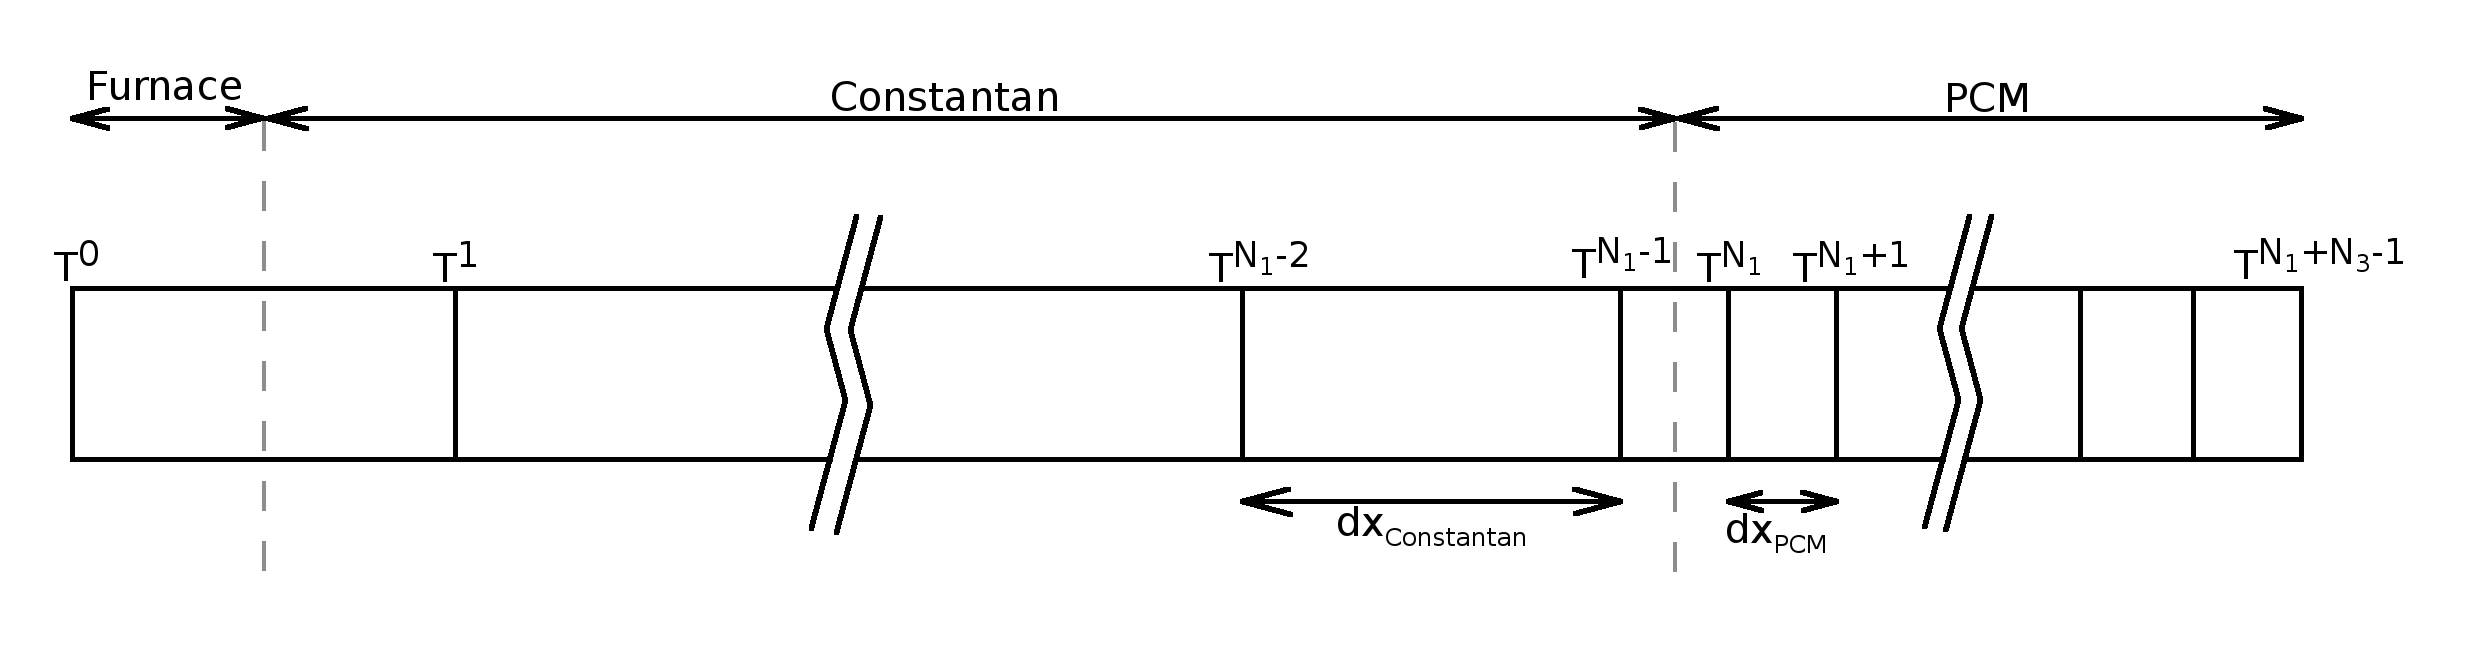
\includegraphics[width=1.\textwidth]{/home/argo/masterarbeit/vortrag/images/discretization_grid.png}
	\caption{}
	\label{fig:mathematical_model_discretized}
\end{figure}

Correspondingly in Fig. \ref{fig:mathematical_model_discretized} one can see the spatially discretized model of the sample side, where on the very left is the furnace. Heat then flows through the silver plate finally into the PCM. Since the furnace is heated in such a way by regulating that the temperature at the reference crucible increases linearly with a heating rate $\beta$ and due to constant material properties of silver with respect to temperature the furnace' temperature increases as well with a constant rate $\beta$. From this follows the first boundary condition

\begin{equation}
	T^0 = T_0 + \beta t
\end{equation}

with a start temperature $T_0$ and the heating rate $\beta$. For the boundary condition at the right hand side we assume that no heat can leave the PCM. So the heat flux is

\begin{equation}
	\Phi_q^{N-1} = \lambda_{pcm} \frac{T^N - T^{N-1}}{\Delta x^N} = 0
\end{equation}

using Fourier's law and a virtual grid point $T^N$. \\
At time $t_0=0$ we assume that the temperature is equal everywhere:

\begin{equation}
	T^i(t_0=0) = T_0 \ \forall \ i \in \{ 0,1,...,N-1 \}
\end{equation}

For the spatial discretization of the heat equation we applied the method of lines. Since the heat conductivity $\lambda$ is constant everywhere, on the RHS of heat equation \eqref{eq:heat_equation} is a second derivative with respect to space. The resulting initial value problem is given by

\begin{align}
\hspace{-2cm}
\frac{d}{dt} \begin{bmatrix*}
T^0 \\[1ex]
T^1 \\[0.3ex]
\vdots \\[1ex]
T^{N-N_{pcm}-2} \\[1.7ex]
T^{N-N_{pcm}-1} \\[1.7ex]
T^{N-N_{pcm}} \\[0.5ex]
\vdots \\[1.5ex]
T^{N-2} \\[1ex]
T^{N-1}
\end{bmatrix*} = &
\begin{bmatrix}
\beta \\
\frac{\lambda_{\text{Ag}}}{\rho_{\text{Ag}} \ c_{p,\text{Ag}}} \cdot \tilde{\Delta} T^1 \\[0.7ex]
\vdots \\[0.3ex]
\frac{\lambda_{\text{Ag}}}{\rho_{\text{Ag}} \ c_{p,\text{Ag}}} \cdot \tilde{\Delta} T^{N-N_{pcm}-1} \\[1.5ex]
\frac{\lambda_{\text{Ag}}}{\rho_{\text{Ag}} \ c_{p,\text{Ag}}} \cdot \tilde{\Delta} T^{N-N_{pcm}} \\[1.5ex]
\frac{\lambda_{\text{pcm}}}{\rho_{\text{pcm}} \ c_{p,{\text{pcm}}}(T^{N-N_{pcm}+1})} \cdot \tilde{\Delta} T^{N-N_{pcm}+1} \\[0.5ex]
\vdots \\[0.5ex]
\frac{\lambda_{\text{pcm}}}{\rho_{\text{pcm}} \ c_{p,{\text{pcm}}}(T^{N-2})} \cdot \tilde{\Delta} T^{N-2} \\[0.5ex]
\frac{\lambda_{\text{pcm}}}{\rho_{\text{pcm}} \ c_{p,\text{pcm}}(T^{N-1})} \cdot \tilde{\Delta} T^{N-1}
\end{bmatrix} \label{eq:heat_equation_discretized} \\[2ex]
T^i(t_0=0) = & \ T_0 \ \ \forall \ \ i \in \{ 0,1,...,N-1 \} \nonumber
\end{align}

where using \eqref{eq:2_point_formula_inhomogeneous} the abbreviation for the discretized second derivative is defined as

\begin{align}
	\tilde{\Delta} T^i := \frac{1}{\Delta x_{i-1}^2} \left[ \frac{2}{1+\alpha_{i-1}} T^{i-1} - \frac{2}{\alpha_{i-1}} T^{i} + \frac{2}{\alpha_{i-1} (\alpha_{i-1} + 1)} T^{i+1} \right]
\end{align}

and the factor coming from the inhomogeneous grid is

\begin{align}
	\alpha_i = \frac{\Delta x_{i+1}}{\Delta x_{i}}
\end{align}

The system is structured in three parts. First there is the furnace which increases its temperature with the heating rate $\beta$. Afterwards comes the silver plate until index $N$-$N_{pcm}$-$1$ and finally the PCM with temperature dependent specific heat capacity $c_p$. \\

Solving \eqref{eq:heat_equation_discretized} yields the temperature but we are primarily interested in the heat flux into the PCM $\varPhi_{q}^{\text{pcm,in}}$ marked in Fig. \ref{fig:mathematical_model_discretized}. For the conversion from temperature to heat flux we use Fourier's law \eqref{eq:fouriers_law} where the gradient is discretized:

\begin{align}
	\varPhi_{q}^{\text{pcm,in}}(T) = & - \bar{\lambda} \frac{T^{N_{\text{pcm}}} - T^{N_{\text{pcm}}-1}}{\Delta x_{N_{\text{pcm}}-1}} \cdot A_{\text{pcm}} \\
	\approx & - \lambda_{\text{pcm}} \frac{T^{N_{\text{pcm}}+1} - T^{N_{\text{pcm}}}}{\Delta x_{N_{\text{pcm}}}} \cdot A_{\text{pcm}} \nonumber
\end{align}

The approximation is necessary because we do not know the heat conductivity $\bar{\lambda}$ at the transition between the silver plate and the PCM. \\
Since Fourier's law gives a heat flux density we need to add a factor of the PCM's cross section $A_{\text{pcm}}$. It is computed by

\begin{equation}
	\frac{m_{pcm}}{N_{pcm}} = m_{pcm,i} = \rho_{pcm} \cdot A_{pcm} \cdot \Delta x_i 
\end{equation}

assuming beside a homogeneous mass distribution, a constant grid size $\Delta x$ in the PCM which is satisfied in good approximation by construction of the spatial discretization grid, see next section. The final equation for the heat flux computation then reads as

\begin{equation}
	\varPhi_{q}^{\text{pcm,in}}(T) \approx - \frac{\lambda_{pcm} \ m_{pcm}}{N_{pcm} \ \rho_{pcm} \ (\Delta x_{N_{pcm}})^2} \left( T^{N_{\text{pcm}}+1} - T^{N_{\text{pcm}}} \right)
	\label{eq:heat_flux_computation_final}
\end{equation}


\subsection{Spatial discretization grid}
\label{sec:spatial_discretization_grid}
At first the spatial discretization grid was constant in the silver and PCM respectively with grid sizes $\Delta x_{\text{Ag}} > \Delta x_{\text{PCM}}$ because only in PCM the phase transition occurs we are interested in. As for the silver plate we get appropriate results for the lengths $L1=40$ and $L3=0.1$ there is a big discontinuity in the grid size at the transition from silver to PCM. In order to avoid numerical problems the used framework of generating a continuous grid will be explained now. \\
In the following $x$ will denote the physical grid, $\tilde{x}$ the computation grid and $\chi(\tilde{x}) = x$ the corresponding mapping which is defined by its derivative

\begin{equation}
	\frac{\partial \chi}{\partial \tilde{x}}(\tilde{x}) := \frac{\Delta \bar{x} - \Delta \underline{x}}{1 + e^{\gamma(\tilde{x} - b)}} + \Delta \underline{x}
\end{equation}

with the parameters $\Delta \underline{x}, \Delta \bar{x}$ as lower and upper bounds of the grid size. $\gamma$ defines the transition shape and $b$ the transition position on the computation grid. Since these parameters are quite counterintuitive they will be calculated with the following parameters:

\begin{itemize}
	\item $N \in \mathbb{N}$: total number of computation grid points.
	\item $n_{pcm} \in (0,1)$: Ratio of grid points for the PCM.
	\item $n_{tr} \in (0,1)$: Ratio of grid points for the transition.
	\item $n_{m} \in (0,1)$: Ratio of grid points: Margin to the PCM, where the transition is finished up to a threshold.
	\item $t < 1$: At grid point $N-N_{pcm}-N_m$, $\frac{\partial \chi(\tilde{x})}{\partial \tilde{x}}$ has finished the transition by $(100 \cdot t)\%$.
\end{itemize}

First of all, the ratios of grid points $n_i$ can be converted easily into absolute numbers with $N_i = N \cdot n_i$. The central position of the grid transition in the computation grid size is

\begin{equation}
	b = N - N_{pcm} - N_m - \frac{1}{2} m_{tr}
	\label{eq:spatial_grid_b}
\end{equation}

Furthermore we get $\gamma$ by

\begin{subequations}
\begin{align}
	\frac{\partial \chi}{\partial \tilde{x}}(\tilde{x}=N-N_{pcm}-N_m) = & \Delta \underline{x} + (\Delta \bar{x} - \Delta \underline{x}) \cdot (1-t) \\
	\Leftrightarrow \frac{\Delta \bar{x} - \Delta \underline{x}}{1 + e^{\gamma(N-N_{pcm}-N_m - b)}} + \Delta \underline{x} = & \Delta \underline{x} + (\Delta \bar{x} - \Delta \underline{x}) \cdot (1-t)  \\
	\stackrel{\eqref{eq:spatial_grid_b}}{\Leftrightarrow}  1 + e^{\gamma \frac{N_{tr}}{2}} = & \frac{1}{1 - t}  \\[2ex]
	\Leftrightarrow \gamma = \frac{2}{N \cdot n_{tr}} \ln(\frac{t}{1-t})
\end{align}
\end{subequations}

The remaining variables $\underline{x}$ and $\bar{x}$ we get by the condition that $T^{N_1-1}$ is at the physical grid position $L_1$

\begin{subequations}
	\begin{align}
	\sum_{i=0}^{N_1 - 2} \frac{\partial \chi}{\partial \tilde{x}}(i) = & L_1 \\
	\Leftrightarrow \sum_{i=0}^{N_1 - 2} \left[ \frac{\Delta \bar{x} - \Delta \underline{x}}{1 + e^{\gamma(i - b)}} + \Delta \underline{x} \right] = & L_1 \\
	\Leftrightarrow \underbrace{ \left[ \sum_{i=0}^{N_1 - 2} \frac{1}{1 + e^{\gamma(i - b)}} \right] }_{=: W_{11}} \cdot \Delta \bar{x} + \underbrace{\left[ N_1 - 1 - \sum_{i=0}^{N_1 - 2} \frac{1}{1 + e^{\gamma(i - b)}} \right]}_{=: W_{12}} \cdot \Delta \underline{x} = & L_1
	\end{align}
\end{subequations}

and $T^{N_1+N_3-1}$ is at the physical grid position $L_1+L_3$

\begin{subequations}
	\begin{align}
	\sum_{i=0}^{N_1 + N_3 - 2} \frac{\partial \chi}{\partial \tilde{x}}(i) = & L_1 + L_3 \\
	\Leftrightarrow \sum_{i=0}^{N_1 + N_3 - 2} \left[ \frac{\Delta \bar{x} - \Delta \underline{x}}{1 + e^{\gamma(i - b)}} + \Delta \underline{x} \right] = & L_1 + L_3 \\
	\Leftrightarrow \underbrace{ \left[ \sum_{i=0}^{N_1 + N_3 - 2} \frac{1}{1 + e^{\gamma(i - b)}} \right] }_{=: W_{21}} \cdot \Delta \bar{x} + \underbrace{ \left[ N_1 + N_3 - 1 - \sum_{i=0}^{N_1 + N_3 - 2} \frac{1}{1 + e^{\gamma(i - b)}} \right] }_{=: W_{22}} \cdot \Delta \underline{x} = & L_1 + L_3
	\end{align}
\end{subequations}

This gives the linear system

\begin{equation}
	\begin{bmatrix}
		W_{11} & W_{12} \\
		W_{21} & W_{22}
	\end{bmatrix}
	\begin{bmatrix}
		\Delta \bar{x} \\
		\Delta \underline{x}
	\end{bmatrix}
	= 
	\begin{bmatrix}
		L_1 \\
		L_1 + L_3
	\end{bmatrix}
\end{equation}
  
 we can solve for $\Delta \bar{x}$ and $\Delta \underline{x}$. Fig. \ref{fig:computation_physical_grid} and \ref{fig:grid_size} show illustrations of the resulting functions for the physical grid $x = \chi(\tilde{x})$ and the gridsize $\Delta x = \frac{\partial \chi}{\partial \tilde{x}}(\tilde{x})$. Although those are discrete functions they are plotted continuously for better comprehensibility. \\



\begin{figure}[H]
	\centering
	\begin{tikzpicture}
	\begin{axis}[domain=0:25,
	samples=100,
	xmin=0, xmax=30,
	ymin=0., ymax=12.,	 
	axis lines=left,
	xtick={15., 25.},
	xticklabels={$N\text{-}1\text{-}N_{pcm}$, $N \text{-} 1$},
	ytick={10.1, 10.75},
	yticklabels={$L_1$, $L_1 + L_3$},
	xlabel=$\tilde{x}$, xlabel style={at=(current axis.right of origin), anchor=west},
	ylabel=\empty
	]
	
	\addplot+[color=black, mark=none] {(1 - 0.05)*(x + 1/0.5 * ln((exp(-0.5*10) + 1) / (exp(0.5*(x-10))+1))) + 0.05*x}
	node[pos=0.95, above, sloped] {$\chi(\tilde{x})$};
	
	\addplot[only marks, mark=x, color=black] 
	table {15	10.1
		   25   10.75
	};	
	
	% L1
	\draw [loosely dashed] (0, 101) -- (150, 101);
	\draw [loosely dashed] (150, 0) -- (150, 101);	
	
	
	% L1 + L3
	\draw [loosely dashed] (0, 107.5) -- (250, 107.5);
	\draw [loosely dashed] (250, 0) -- (250, 107.5);	
	
	
	\end{axis}
	\end{tikzpicture}
	\caption{Mapping of the physical grid $x=\chi(\tilde{x})$ as a function of the computation grid $\tilde{x}$.}
	\label{fig:computation_physical_grid}
\end{figure}






\begin{figure}[H]
	\centering
	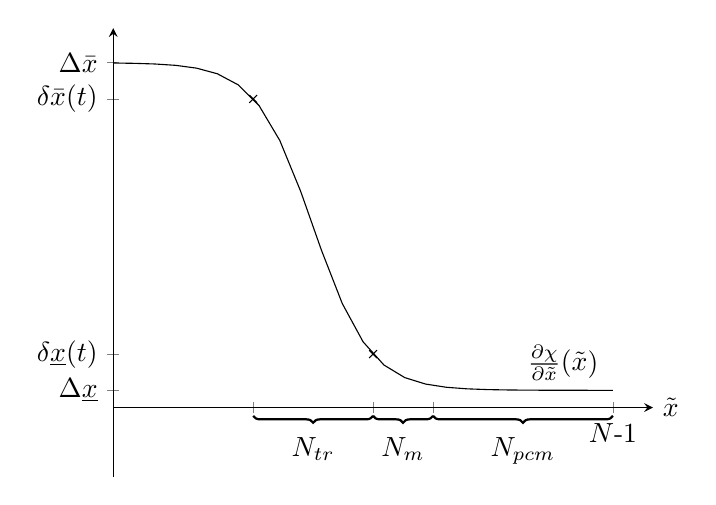
\begin{tikzpicture}
	\begin{axis}[
	axis x line = middle,
	axis y line = middle,
	xtick={7,13,16,25},
	ytick={0.05, 1., 0.155, 0.895},
	xticklabels={, , , $N\text{-}1$},
	yticklabels={$\Delta \underline{x}$, $\Delta \bar{x}$, $\delta \underline{x}(t)$, $\delta {\bar{x}}(t)$},
	xmin=0, xmax=27,
	ymin=-0.2, ymax=1.1,
	xlabel=$\tilde{x}$, xlabel style={at=(current axis.right of origin), anchor=west},
	]
	\addplot [domain=0:25] {(1 - 0.05) / (exp(0.7*(x-10))+1) + 0.05} node[pos=0.9, above, sloped] {$\frac{\partial \chi}{\partial \tilde{x}}(\tilde{x})$};
	
	\draw [thick,decoration={brace,mirror,raise=3pt},decorate] 
	(axis cs:16,0) --
	node[below=7pt] {$N_{pcm}$} 
	(axis cs:25,0);
	
	\draw [thick,decoration={brace,mirror,raise=3pt},decorate] 
	(axis cs:13,0) --
	node[below=7pt] {$N_{m}$} 
	(axis cs:16,0);
	
	\draw [thick,decoration={brace,mirror,raise=3pt},decorate] 
	(axis cs:7,0) --
	node[below=7pt] {$N_{tr}$} 
	(axis cs:13,0);

	\addplot[only marks, mark=x, color=black] 
	table {7	0.895
	       13   0.155
	};	
	
	% L1
	\draw [loosely dashed] (0, 109.5) -- (70, 109.5);
	\draw [loosely dashed] (70, 20) -- (70, 109.5);	
	
	% L1 + L3
	\draw [loosely dashed] (0, 35.5) -- (130, 35.5);
	\draw [loosely dashed] (130, 20) -- (130, 35.5);	

	
	
	
	\end{axis}
	\end{tikzpicture}
	\caption{Mapping of the gridsize $\Delta x = \frac{\partial \chi}{\partial \tilde{x}}(\tilde{x})$ as a function of the computation grid. $N_{pcm}$, $N_m$ and $N_{tr}$ are the total discretization points for the PCM, margin and grid transition part. Start $\delta \bar{x}(t) := \Delta \underline{x} + (\Delta \bar{x} - \Delta \underline{x})\cdot t$ and end $\delta \underline{x}(t) := \Delta \underline{x} + (\Delta \bar{x} - \Delta \underline{x})\cdot(1-t)$ of the grid transition are marked.}
	\label{fig:grid_size}
\end{figure}


\subsection{Analytical solution of reference side}

The measurement data for the residuum computation is given as a function dependent on the temperature at the reference crucible $T_{ref}^{\eta_i}$. Since we need to evaluate the solution of the heat equation (PCM side) at the corresponding time points $t_i$ it is necessary to calculate these.
This is done by applying Newton's method on the heat equation's solution of the reference side which can be solved analytically as follows. \\

As the crucible of the reference side is empty there is just the silver plate with a constant temperature coefficient $a$. The start and boundary conditions are equal to the ones of the PCM side. So the boundary value problem reads 

\begin{subequations}
	\begin{empheq}[box=\widefbox]{align}
		\frac{\partial T}{\partial t}(x,t) & - a \cdot \frac{\partial^2 T}{\partial x^2}(x,t) = 0 \label{eq:analytical_soln_pde} \\
		T(0,t) & = T_0 + \beta \cdot t \label{eq:analytical_soln_bc_neumann} \\
		\frac{\partial T}{\partial x}(L_1,t) & = 0 \label{eq:analytical_soln_bc_dirichlet}  \\
		T(x,0) & = T_0 
	\end{empheq}
\end{subequations}

The first step is a separate ansatz of the solution function $T(x,t)$ with $\bar{T}(x,t)$ satisfying the boundary conditions:

\begin{align}
	{T}(x,t) = \bar{T}(x,t) + \Gamma(x,t) \\
	\bar{T}(x,t) = A(t) + B(t) \cdot x
\end{align}

Inserting the boundary conditions and a coefficient comparison in $x$ gives

\begin{align}
	\bar{T}(0,t) = T_0 + \beta \cdot t = A(t) \\
	\frac{\partial \bar{T}}{\partial x}(L_1,t) = 0 \cdot x = B(t)
\end{align}

\begin{equation}
	\Rightarrow \bar{T}(x,t) = T_0 + \beta \cdot t
\end{equation}


By construction this leads to homogenous boundary conditions of $\Gamma(x,t)$:

\begin{align}
	T(0,t) & = \bar{T}(0,t) + \Gamma(0,t) = T_0 + \beta \cdot t + \Gamma(0,t) \stackrel{\eqref{eq:analytical_soln_bc_dirichlet}}{=} T_0 + \beta \cdot t \\
	 &\Rightarrow \Gamma(0,t) = 0 \\[2ex]
	\frac{\partial T}{\partial x}(L_1,t) & = \underbrace{\frac{\partial \bar{T}}{\partial x}(L_1,t)}_{= 0} + \frac{\partial \Gamma}{\partial x}(L_1,t) \stackrel{\eqref{eq:analytical_soln_bc_neumann}}{=} 0 \\
	 &\Rightarrow \frac{\partial \Gamma}{\partial x}(L_1,t) = 0
\end{align}


Inserting $\bar{T}$ and $\Gamma$ into \eqref{eq:analytical_soln_pde} gives

\begin{align}
	\frac{\partial \bar{T}}{\partial t} + \frac{\partial \Gamma}{\partial t} - a \left[ \frac{\partial^2 \bar{T}}{\partial x^2} + \frac{\partial^2 \Gamma}{\partial x^2} \right] = 0
\end{align}
	

	
	
With $\frac{\partial \bar{T}}{\partial t} = \beta$, $\frac{\partial^2 \bar{T}}{\partial x^2} = 0$ and

\begin{align}
T(x,0) & = \underbrace{\bar{T}(x,0)}_{T_0} + \Gamma(x,0) = T_0 \\
& \Rightarrow \Gamma(x,0) = 0
\end{align}

this leads to the boundary value problem in $\Gamma(x,t)$

\begin{subequations}
	\begin{empheq}[box=\widefbox]{align}
		\frac{\partial \Gamma}{\partial t}(x,t) - a \cdot \frac{\partial^2 \Gamma}{\partial x^2}(x,t) & = - \beta =: \bar{q} \label{eq:analytical_soln_pde_gamma} \\
		\Gamma(0,t) & = 0 \label{eq:analytical_soln_bc_neumann_gamma} \\
		\frac{\partial \Gamma}{\partial x}(L1,t) & = 0 \label{eq:analytical_soln_bc_dirichlet_gamma}  \\
		\Gamma(x,0) & = 0 =: \bar{f}
	\end{empheq}
	\label{eq:analytical_soln_gamma}
\end{subequations}


The homogeneous solution (i.e. $\bar{q}=0$) can be obtained by an ansatz of seperation of variables $\Gamma(x,t) = \mathcal{T}(t) \cdot X(x)$, \eqref{eq:analytical_soln_pde_gamma} is then equivalent to

\begin{equation}
	\dot{\mathcal{T}} X = a \mathcal{T} X'' \quad \Leftrightarrow \quad \frac{1}{a} \frac{\dot{\mathcal{T}}}{\mathcal{T}} = \frac{X''}{X} = const =: - \lambda
\end{equation}


since the LHS $\sfrac{\dot{\mathcal{T}}}{{\mathcal{T}}}$ just depends in $t$ and the RHS $\sfrac{X''}{X}$ just depends on $x$. 

The solution of the ordinary differential equation $X'' = - \lambda \cdot X$ is

\begin{equation}
	X(x) = c_1 \cdot \sin(\sqrt{\lambda} x) + c_2 \cdot \cos(\sqrt{\lambda} x)
\end{equation}

where $c_1$ and $c_2$ are determined by the boundary conditions $X(0) = 0$ and $X'(L_1) = 0$:

\begin{align}
	X(0) = c_2 \stackrel{!}{=} 0 \\
	X'(L_1) = \left. c_1 \sqrt{\lambda} cos(\sqrt{\lambda} x) \right|_{x=L_1} = c_1 \sqrt{\lambda} cos(\sqrt{\lambda} L_1) \stackrel{!}{=} 0 \\
	\Rightarrow \sqrt{\lambda_n} = \frac{(2n -1)\pi}{2 L_1} \qquad n=1,2,...
\end{align}

The general solution of $X_n(x)$ is then given by

\begin{equation}
	\tilde{X}_n(x) = c_1 \cdot \sin\left(\frac{(2n -1)\pi}{2 L_1} \cdot x\right) =: c_1 \cdot X_n(x)
\end{equation}

In order to solve the non-homogeneous boundary value problem \eqref{eq:analytical_soln_gamma} $\Gamma$, $\bar{q}$ and $\bar{f}$ are expanded in a Fourier series with $X_n(x)$ as basis where $c_1$ is incorporated in the corresponding Fourier coefficient:

\begin{subequations}
	\centering
	\begin{align}
		\Gamma(x,t) & = \sum_{n=1}^{\infty} \mathcal{T}_n(t) X_n(x) \\
		\bar{q}(x,t) & = \sum_{n=1}^{\infty} \bar{q}_n(t) X_n(x) \\
		\bar{f}(x) & = \sum_{n=1}^{\infty} \bar{f}_n X_n(x)
	\end{align}
\end{subequations}

The Fourier coefficients $\bar{q}_n(t)$ and $\bar{f}_n$ are then computed by

\begin{subequations}
	\begin{align}
		\bar{q}_n(t) & = \frac{\int_{0}^{L_1} \bar{q}(x,t) X_n(x) dx}{\int_{0}^{L_1} X_n^2(x) dx} \ \overbrace{=}^{\bar{q}=-\beta} \ - \frac{4 \beta}{\pi (2n - 1)} \\
		\bar{f}_n & = \frac{\int_{0}^{L_1} \bar{f}(x) X_n(x) dx}{\int_{0}^{L_1} X_n^2(x) dx} \ \underbrace{=}_{\bar{f}=0} 0
	\end{align}
\end{subequations}

Inserting this into \eqref{eq:analytical_soln_pde_gamma} gives us

\begin{align*}
	\sum_{n=1}^{\infty} \dot{\mathcal{T}}_n(t) X_n(x) - a \sum_{n=1}^{\infty} \mathcal{T}_n(t) X_n''(x) = \sum_{n=1}^{\infty} \bar{q}_n(t) X_n(x) \nonumber \\
	\stackrel{X'' = - \lambda X}{\Leftrightarrow} \ \ \sum_{n=1}^{\infty} \dot{\mathcal{T}}_n(t) X_n(x) + a \sum_{n=1}^{\infty} \lambda_n \mathcal{T}_n(t) X_n(x) = \sum_{n=1}^{\infty} \bar{q}_n(t) X_n(x)
\end{align*}

With a coefficient comparison in $X_n$ we get the inhomogeneous ODE

\begin{equation}
	\dot{\mathcal{T}_n}(t) + a \lambda_n \mathcal{T}_n(t) = \bar{q}_n(t)
	\label{eq:analytical_soln_inhomo_ode}
\end{equation}

where the solution of the homogeneous part (i.e. $\bar{q}_n(t) = 0$) is

\begin{equation}
	\mathcal{T}_n^h(t) = A_n \cdot e^{-a \lambda_n t}
\end{equation}

Applying the method of variation of constants by setting $A_n = A_n(t)$ and inserting in \eqref{eq:analytical_soln_inhomo_ode} gives

\begin{align}
	\dot{A_n}(t) & = \bar{q}_n(t) \cdot e^{a \lambda_n t} = -\frac{4 \beta}{\pi (2n - 1)} e^{a \lambda_n \tau} \\
	\Rightarrow A_n(t) & = \int_{0}^{t} -\frac{4 \beta}{\pi (2n - 1)} e^{a \lambda_n \tau} d \tau + A_{n,c} \\
	& = -\frac{4 \beta}{\pi (2n - 1)} \frac{1}{a \lambda_n} \left[ e^{a \lambda_n t} - 1 \right] + A_{n,c}
\end{align}

The solution of the inhomogeneous ODE \eqref{eq:analytical_soln_inhomo_ode} then is
\begin{align}
	\mathcal{T}_n(t) & = A_n(t) \cdot e^{-a \lambda_n t}  \\
	& = -\frac{4 \beta}{\pi (2n - 1)} \frac{1}{a \lambda_n} \left[1 - e^{-a \lambda_n t} \right] + A_{n,c} e^{- a \lambda_n t} \nonumber
\end{align}

The remaining unknown $A_{n,c}$ is determined by considering the Fourier series of the starting condition

\begin{equation}
	\Gamma(x,t) = \sum_{n=1}^{\infty} \mathcal{T}_n(0) X_n(x) = \sum_{n=1}^{\infty} \bar{f}_n X_n(x) = \bar{f}(x)
\end{equation}

From $\mathcal{T}_n(0) = A_{n,c}$, $\bar{f}_n=0$ and again a coefficient comparison it follows that

\begin{equation}
	A_{n,c} = 0
\end{equation}

Finally the solution of the boundary value problem \eqref{eq:analytical_soln_pde} of the reference side reads as

\begin{align}
	& \ \ T(x,t) = \bar{T}(x,t) + \Gamma(x,t) \nonumber \\
	\Leftrightarrow \ \ & T(x,t) = T_0 + \beta \cdot t + \sum_{n=1}^{\infty} \mathcal{T}_n(t) X_n(x) \nonumber \\[1ex]
	\Leftrightarrow \ \ & \raalign{}{T(x,t) = T_0 + \beta \cdot t - \sum_{n=1}^{\infty} \left\{ \frac{4 \beta}{\pi (2n - 1)} \frac{1}{a \cdot \lambda_n} \left[ 1 - e^{- a \lambda_n t} \right] \cdot \sin(\sqrt{\lambda_n} \cdot x) \right\}} \label{eq:analytical_soln_final_formula}
\end{align}



\section{Parameter estimation of specific heat capacity $c_p$}





\subsection{Parametrization of $c_p$}
Since in the end we want to estimate the specific heat capacity $c_p$ we need a parametrization with enough degrees of freedom in order to generate appropriate functions. 

\subsubsection{NURBS}
\label{sec:nurbs}
In early stages of work we used Non-Uniform Rational B-Splines (NURBS). The generated curve $C(u) = \{C^x(u), C^y(u) \} \in \mathbb{R}^2$ is defined by

\begin{equation}
	C(u) = \frac{\sum_{i=0}^{n} N_{i,p}(u) \omega_i P_i }{\sum_{i=0}^{n} N_{i,p}(u) \omega_i} \qquad a \le u \le b
\end{equation}

where $P_i = \{ P_i^x, P_i^y \} \in \mathbb{R}^2$ are called control points, $\omega_i$ are weights for each control point and $N_{i,p}(u)$ are the B-Spline basis functions. These are defined recursively by

\begin{align}
	N_{i,p}(u) = & \frac{u - u_i}{u_{i+p} - u_i} N_{i,p-1}(u) + \frac{u_{i+p+1} - u}{u_{i+p+1} - u_{i+1}} N_{i+1,p-1}(u) \label{eq:NURBS_basis_polynomial} \\[1ex]
	N_{i,0} = &
	\begin{cases}
		1 \quad \text{if } u_i \le u < u_{i+1} \\
		0 \quad \text{otherwise}
	\end{cases} \nonumber
\end{align}

where $u_i$ are the elements of the knot vector

\begin{equation}
	U = \{u_0,...,u_m\}=\{a,...,a,u_{p+1},...,u_{m-p-1},b,...,b\}.
\end{equation}

With this formulation there are $n+1$ control points, $p$ is the order of the basis functions and the order of the resulting curve is defined by $p+1$. The interval $[a,b]$ is arbitrary in the sense that for $C(u=a)=P_0$,  $C(u=b)=P_n$ and $u \in (a,b)$ are points between depending on the knot vector.\\

In our experimental setup we used a NURBS order of $4$, i.e. $p=3$. $a=0$ and $b=1$ so $u \in [0,1]$ and the knot vector is linearly increasing, i.e. $U = \{ 0,0,0,0,\frac{1}{n p},\frac{2}{n p},...,\frac{n p - 1}{n p},1,1,1,1 \}$. All control points contribute equally such that $\omega_i=1 \ \forall \ i$. With these settings it holds that $C(u) \in \mathcal{C}^2$.

Since $C(u)$ is a parametrized curve we get a function $c_p(T)$ by using $C^x(u)$ as the domain of definition (temperature) and $C^y(u)$ as the co-domain ($c_p$). Evaluating $C(u)$ on an appropriate fine grid for values of $u$ and subsequently piecewise linear interpolation gives the wanted quantity $c_p(T)$.
The x-coordinates of the control points were fixed on a predefined grid with $P_i^x < P_{i+1}^x$ to guarantee a well-defined function.
As optimization variables we used the corresponding y-coordinates $P_i^y$.

\subsubsection{Fraser-Suzuki Peak}
A parametrization with fewer degrees of freedom and used in general for chromatography and spectroscopy distributions is the Fraser-Suzuki peak \cite{fraser_suzuki_1} \cite{fraser_suzuki_many_fcts}

\begin{align}
	c_p(T) =
	\begin{cases}
		h \cdot \exp \left\{ - \frac{\ln(r)}{\ln(sr)^2} \cdot \left[ \ln\left( 1 + (T-z) \cdot \frac{sr^2 - 1}{wr \cdot sr} \right) \right]^2 \right\} + m \cdot T + b \ & \text{for } \ T < z - \frac{wr \cdot sr}{sr^2 - 1} \\
		m \cdot T + b \ & \ \text{else}
	\end{cases}
	\label{eq:fraser_suzuki}
\end{align}

where $h$, $r$, $sr$, $wr$ and $z$ are the parameters of Fraser-Suzuki. Furthermore the parameters for a linear part $m$ and a constant part $b$ were added. In order to keep the argument of the logarithm positive it must hold $0 < sr < 1$ and $wr > 0$.

\begin{figure}[H]
	\centering
	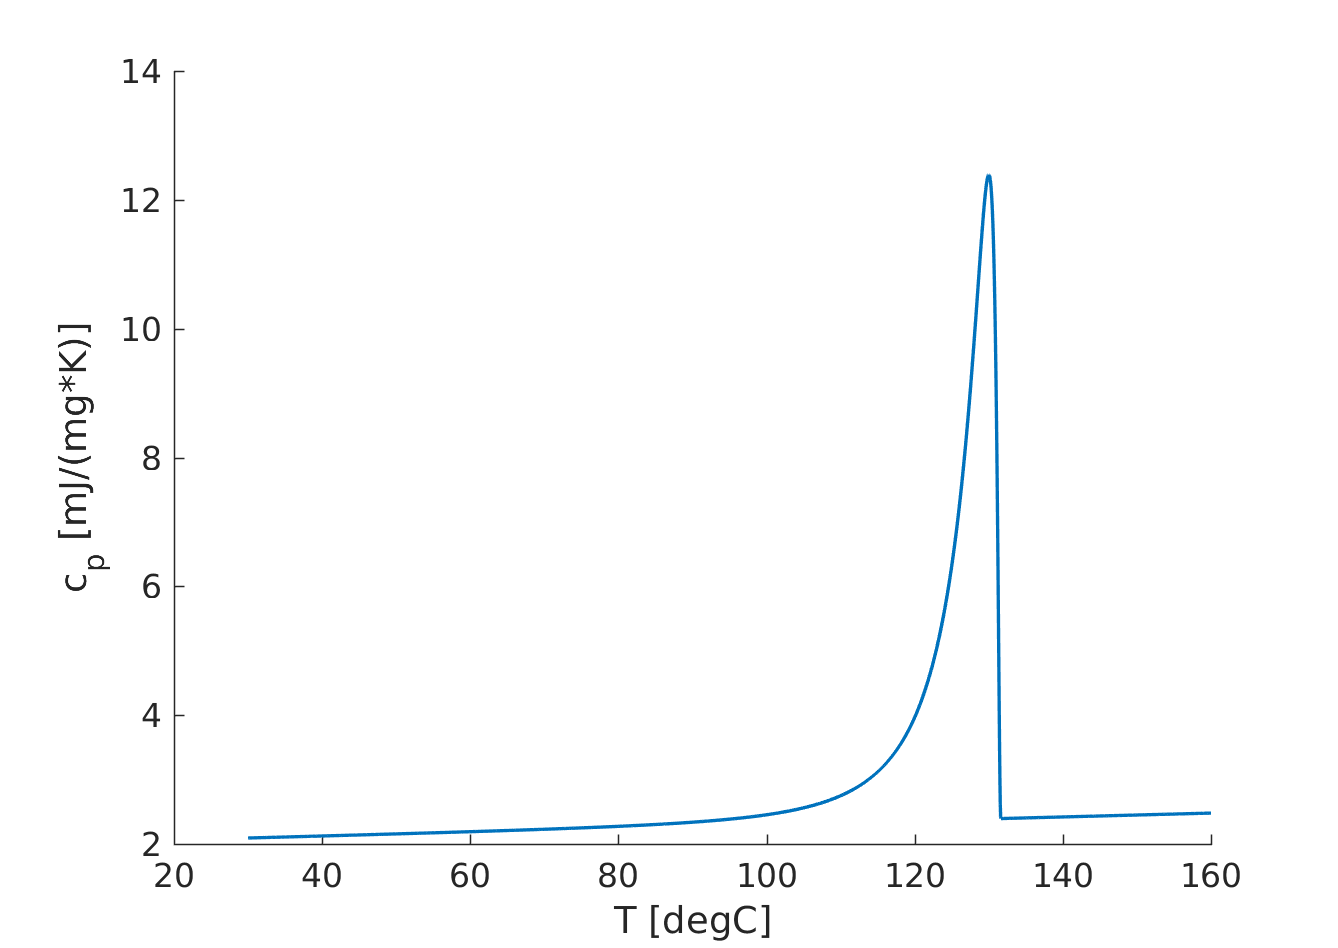
\includegraphics[width=0.8\textwidth]{/home/argo/masterarbeit/thesis/images/fraser_suzuki_example.png}
	\caption{Example of Fraser-Suzuki peak with $h=10$, $r=2$, $wr=5$, $sr=0.3$, $z=130$, $m=0.003$, $b=2$.}
	\label{fig:parametrization_example_fraser_suzuki}
\end{figure}



\subsubsection{Linear combination of Gaussian functions}
As we switched for the derivative computation with respect to the optimization variables from finite differences to IND, implementation problems with NURBS occurred. 
The case structure of the basis polynomial \eqref{eq:NURBS_basis_polynomial} conducts to switch the RHS of the differential equation. This is only supported by the $condassign(a,b,c,d)$ function which assigns $a=c$ if $b>0$ and $a=d$ else. Additionally to $N_{i,0}$ the denominators need this $condassign$ command in order to check for a division by zero. 
Furthermore the piecewise interpolation of the resulting curve $C(u)$ could be realized as well with the $condassign$ command but in total this leads to a lot of unnecessary numerical operations and makes the program quite complex. \\
An alternative simple parametrization which is similar flexible than NURBS is a linear combination of Gaussian functions which is stated in \eqref{eq:parametrization_linear_comb_Gauss}. Per Gaussian there are three optimization variables: Amplitude $A_i$, a shift in the $T$-axis $T_{\text{offset}_i}$ and the standard deviation $\sigma_i$. Additionally there is a linear and constant part with variables $m$ and $b$. So in total there are $3 \cdot n_{\text{Gauss}} + 2$ optimization variables. \\


\begin{equation}
	c_p(T) = \sum_{i=1}^{n_{\text{Gauss}}} A_i \exp\left(- \frac{(T - T_{\text{offset}_i})^2}{\sigma_i^2}\right) + m \cdot T + b
	\label{eq:parametrization_linear_comb_Gauss}
\end{equation} \\

An example $c_p(T)$ function generated by this parametrization is shown in Fig. \ref{fig:parametrization_example_linear_comb_gauss}


\begin{figure}[H]
	\centering
	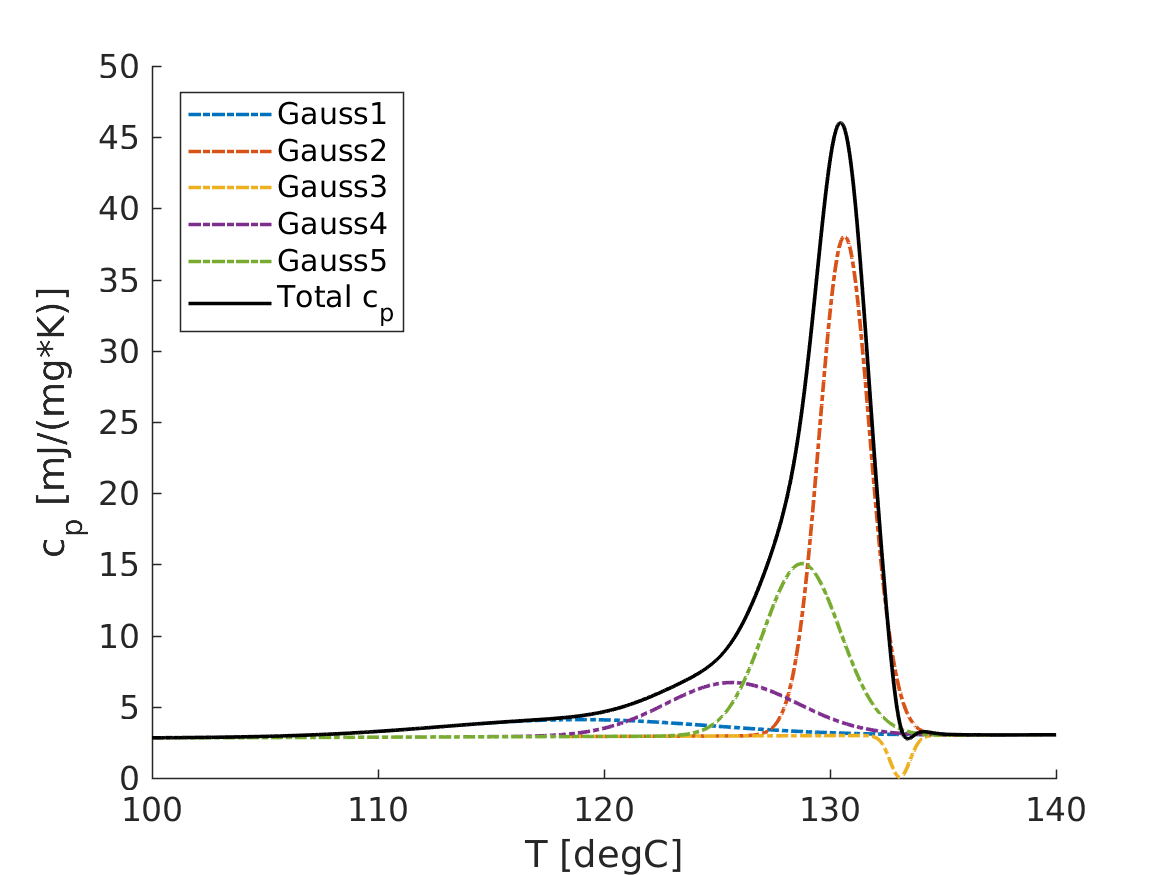
\includegraphics[width=0.8\textwidth]{/home/argo/masterarbeit/thesis/images/c_p_example.png}
	\caption{Example of 5 Gaussians reconstructing a Fraser-Suzuki peak. Each individual Gaussian and total resulting function is plotted where the linear and constant part is included each time.}
	\label{fig:parametrization_example_linear_comb_gauss}
\end{figure}









\subsection{Optimization problem}
In order to perform the parameter estimation for $c_p(T)$ we need to solve the least squares optimization problem

\begin{align}
	\min_{p_{c_p}} \ & \sum_{i=1}^{n_{mp}} \left(  \varPhi_{q}^{pcm,in}(T(t_i;T_0,p_{c_p})) - \varPhi_q^{\eta_i} \right)^2 \\
	s.t. \ & \quad \  \dot{T} = f(T,t;p_{c_p}) \nonumber \\
	& T(0) = T_0 \nonumber \\
	& p_{c_p} \le \bar{p}_{c_p} \nonumber \\
	& p_{c_p} \ge \underline{p}_{c_p} \nonumber
	\label{eq:parameter_estimation_least_squares_problem}
\end{align}

where $p_{c_p} \in \mathbb{R}^{n_p}$ are optimization variables parametrizing the specific heat capacity $c_p(T)$, $n_{{mp}}$ is the number of measurement points, $\varPhi_{q}^{pcm,in}$ is the simulated heat flux into the PCM from the solution of the heat equation $T(t_i;T_0,p_{c_p})$ and $\varPhi_q^{\eta_i}$ is the heat flux measurement value at measurement time $t_i$. The side condition $\dot{T} = f(T,t;p_{c_p})$ with $T(0) = T_0$ is equal to the initial value problem \eqref{eq:heat_equation_discretized} of solving the heat equation. $\bar{p}_{c_p}$ and $\underline{p}_{c_p}$ are upper respectively lower bounds of the optimization variables. \\

The measurement data is given as $\varPhi_q^{\eta_i}(T_{ref}^{\eta_i})$ where $T_{ref}^{\eta_i}$ is the temperature at the reference crucible at measurement time $t_i$. Since we need to pass these times $t_i$ to the differential equation solver for the evaluation of the temperature and sensitivities we obtain them by solving the non-linear equation 

\begin{align}
	T_{ref}^{\eta_i} - T_{ref}^{sim}(t_i) = 0 \quad \forall \ i \in \{1,2,...,n_{mp}\}
\end{align}

using Newton's method where $T_{ref}^{sim}(t)$ is the analytical solution of the heat equation on the reference side \eqref{eq:analytical_soln_final_formula}. This is depicted in Fig. \ref{fig:obtaining_measurement_times}.


\begin{figure}[H]
	\centering
	\begin{tikzpicture}
	\begin{axis}[domain=0:65,
	samples=100,
	xmin=0, xmax=70,
	ymin=0.,	 
	axis lines=left,
	xtick={40},
	xticklabels={$t_i$},
	ytick={0.7, 3.7},
	yticklabels={$T_0$, $T_{ref}^{\eta_i}$},
	xlabel=$time$, xlabel style={at=(current axis.right of origin), anchor=west},
	ylabel=\empty
	]
	
	\addplot+[color=black, mark=none] {0.7 + 0.1*x}
	node[pos=0.87, above, sloped] {$T_{{furnace}}$};
	
	\addplot+[color=black, mark=none] {0.7 + 0.1*x - (1 - exp(-0.11*x)}
	node[pos=0.95, below, sloped] {$T_{{ref}}^{{sim}}$};
	
	\addplot[only marks, mark=x, color=black] 
	table {40 3.7
	};	
	
	\draw [loosely dashed] (0, 370) -- (400, 370);
	\draw [loosely dashed] (400, 0) -- (400, 370);	
	
	\end{axis}
	\end{tikzpicture}
	\caption{}
	\label{fig:obtaining_measurement_times}
\end{figure}


\begin{flushright}
	
\end{flushright}
For the optimization process using Gauss-Newton method (see section \ref{sec:Gauss_Newton}) we first define the residuum vector which euclidean norm $|| \cdot ||_2^2$ will be minimized as 

\begin{equation}
	F_1(p_{c_p}) :=
	\begin{pmatrix}
		\varPhi_{q}^{pcm,in}(T(t_1;T_0,p_{c_p})) - \varPhi_q^{\eta_1} \\
		\textcolor{white}{} \\
		\vdots \\
		\textcolor{white}{} \\
		\varPhi_{q}^{pcm,in}(T(t_{n_{mp}};T_0,p_{c_p})) - \varPhi_q^{\eta_{n_{mp}}}
	\end{pmatrix}
\end{equation} \\


By applying the chain rule we get the corresponding Jacobian

\begin{equation}
	J_1(p_{c_p}) := \frac{\partial F_1}{\partial p_{c_p}} =
	\begin{pmatrix}
		\frac{\partial \varPhi_{q}^{pcm,in}}{\partial T}(T(t_1)) \cdot \frac{\partial T}{\partial p_{c_p}}(t_1) \\
		\textcolor{white}{} \\
		\vdots \\
		\textcolor{white}{} \\
		\frac{\partial \varPhi_{q}^{pcm,in}}{\partial T}(T(t_{n_{mp}})) \cdot \frac{\partial T}{\partial p_{c_p}}(t_{n_{mp}}) \\
	\end{pmatrix}
	\label{eq:optimization_jacobian}
\end{equation}

with

\begin{align}
	\frac{\partial \varPhi_{q}^{pcm,in}}{\partial T}(T(t_i)) = - \frac{\lambda_{pcm} \ m_{pcm}}{N_{pcm} \ \rho_{pcm} \ (\Delta x_{N_{pcm}})^2}
	\begin{pmatrix}
	0 & ... & 0 & -1 & +1 & 0 & ... & 0
	\end{pmatrix}\\
	\forall \ i \in \{1,...,n_{mp} \} \nonumber
\end{align}

using \eqref{eq:heat_flux_computation_final}. The non-zero entries are in column $N_{pcm}$ and $N_{pcm}+1$. \\
The sensitivities $\frac{\partial T}{\partial p_{c_p}}(t_i) \in \mathbb{R}^{N \times n_p}$ are obtained by internal numerical differentiation while solving the differential equation in forward mode with the software SolvIND \cite{diss_jan}. \\




\section{Numerical experiments and results}
All conducted numerical experiments involve the following subproblems: The numerical integration where we solve \eqref{eq:heat_equation_discretized} gives us the temperature $T$ and sensitivities $\frac{\partial T}{\partial p}$. This was accomplished with the numerical integrator DAESOL-II embedded in SolvIND. The integration tolerance was set to $10^{-7}$ and the sensitivities were obtained in forward mode.
The heat flux $\varPhi_q^{pcm,in}$ is then computed with \eqref{eq:heat_flux_computation_final} and the optimization Jacobian $J_1(p_{c_p})$ with \eqref{eq:optimization_jacobian} \todo{Approx.-fehler vom heat flux nimmt mit steigendem N3 ab, bei Vergleich von N3=50 -> 200 hat sich nichts grossartig veraendert -> N3=50 reicht aus}. The parameter estimation is then performed by solving the least squares problem \eqref{eq:parameter_estimation_least_squares_problem}. \todo{welches programm fuer die optimierung} \\
At solving the reference side with the analytical solution \eqref{eq:analytical_soln_final_formula} we stopped the actually infinite sum after 100 summands since the summand is proportional to $n^{-3}$. \\

The material properties used throughout were for silver $c_{p,Ag}=0.235 \frac{mJ}{mg \ K}$, $\rho_{Ag}=10.49 \frac{mg}{mm^3}$ and $\lambda_{Ag}=430 \frac{mW}{mm \ K}$ and for the PCM $\rho_{pcm}=0.85 \frac{mg}{mm^3}$ and $\lambda_{pcm}=0.96 \frac{mW}{mm \ K}$. The initial temperature was set to $T_0=10^\circ C$ and the simulation stopped for the furnace temperature $T^0=200^\circ C$ such that the phase transition is completely finished. \\

Except the forward simulation with an equidistant grid as reference for the error analysis of different spatial grids, all experiments have been done on my laptop using Linux Ubuntu Mate, 2 Cores Intel(R) Core(TM) i3-4100M CPU @ 2.50GHz and 8GB RAM. Former was computed on the IWR-Compute Server Quadxeon2 (4 x Dual Core E7220 2.93 GHz, 256 GB RAM).


\subsection{Smearing effect on simulated heat flux for different heat rates}
The first basic numerical experiment consists of showing that our mathematical model is capable of reproducing heat fluxes exhibiting the smearing effect similar to those measured (see Sec \ref{sec:smearing_problem}). This was achieved by a forward simulation for several different heat rates using  the same specific heat capacity (see Fig. \ref{fig:smearing_effect_c_p}) each time. \\
The resulting heat fluxes for all heat rates from the forward simulation can be seen in Fig. \ref{fig:smearing_effect_simulation_heat_flux}. They exhibit obviously a widening of the peak and a shift of the maximum to higher temperatures for increasing heat rates similar to the measured heat fluxes shown in Fig. \ref{fig:smearing_effect_measurement_heat_flux}. \\
This result forms the basis of reproducing the heat flux measurement values in the simulation and in the further numerical experiments perform a parameter estimation to obtain the specific heat capacity. 



\begin{figure}[H]
	\centering
	\begin{subfigure}{0.9\textwidth}
		\centering
		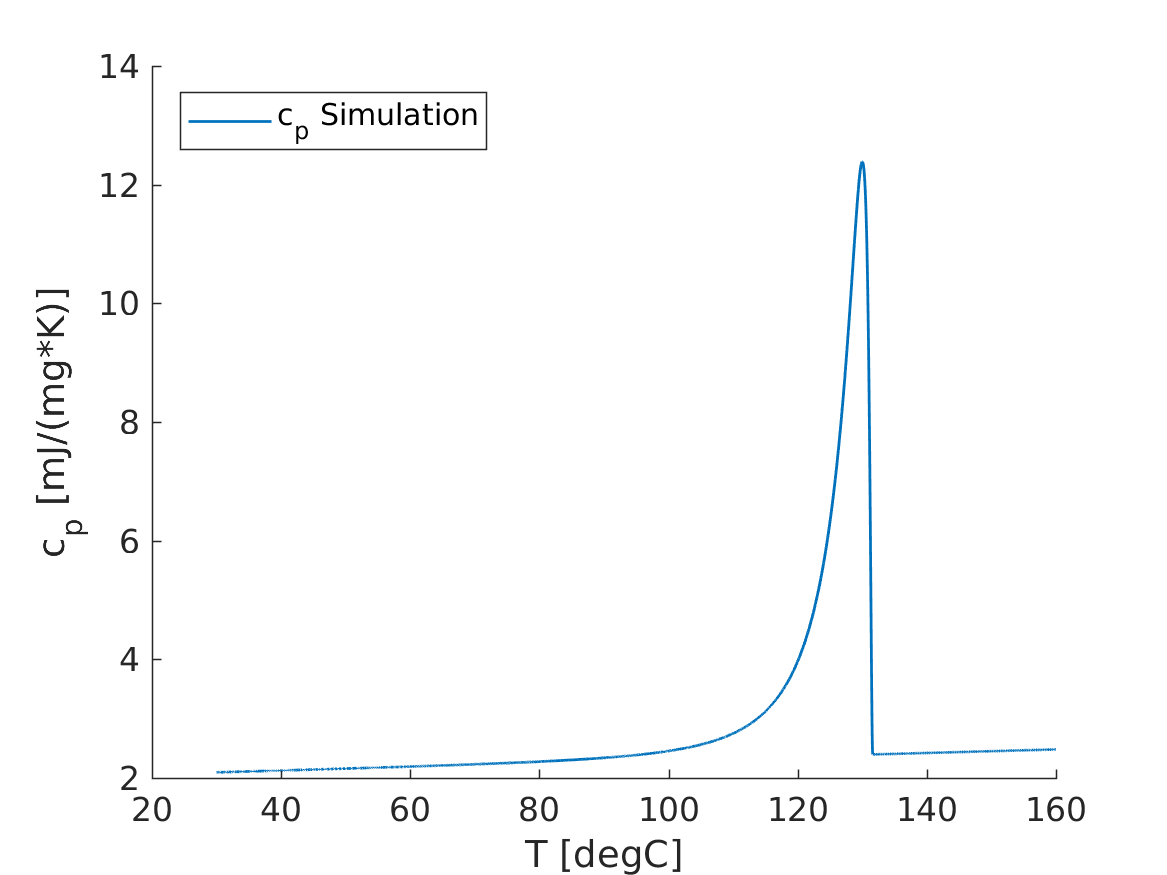
\includegraphics[width=0.5\textwidth]{/home/argo/masterarbeit/thesis/images/smearing_effect_simulation_c_p.png}
		\caption{Used specific heat capacity for all heat rates. Parametrization is Fraser-Suzuki with $h=10$, $r=2$, $wr=5$, $sr=0.3$, $z=130$, $m=0.003$ and $b=2$.}
		\label{fig:smearing_effect_c_p}
	\end{subfigure} \\
	\begin{subfigure}{0.49\textwidth}
		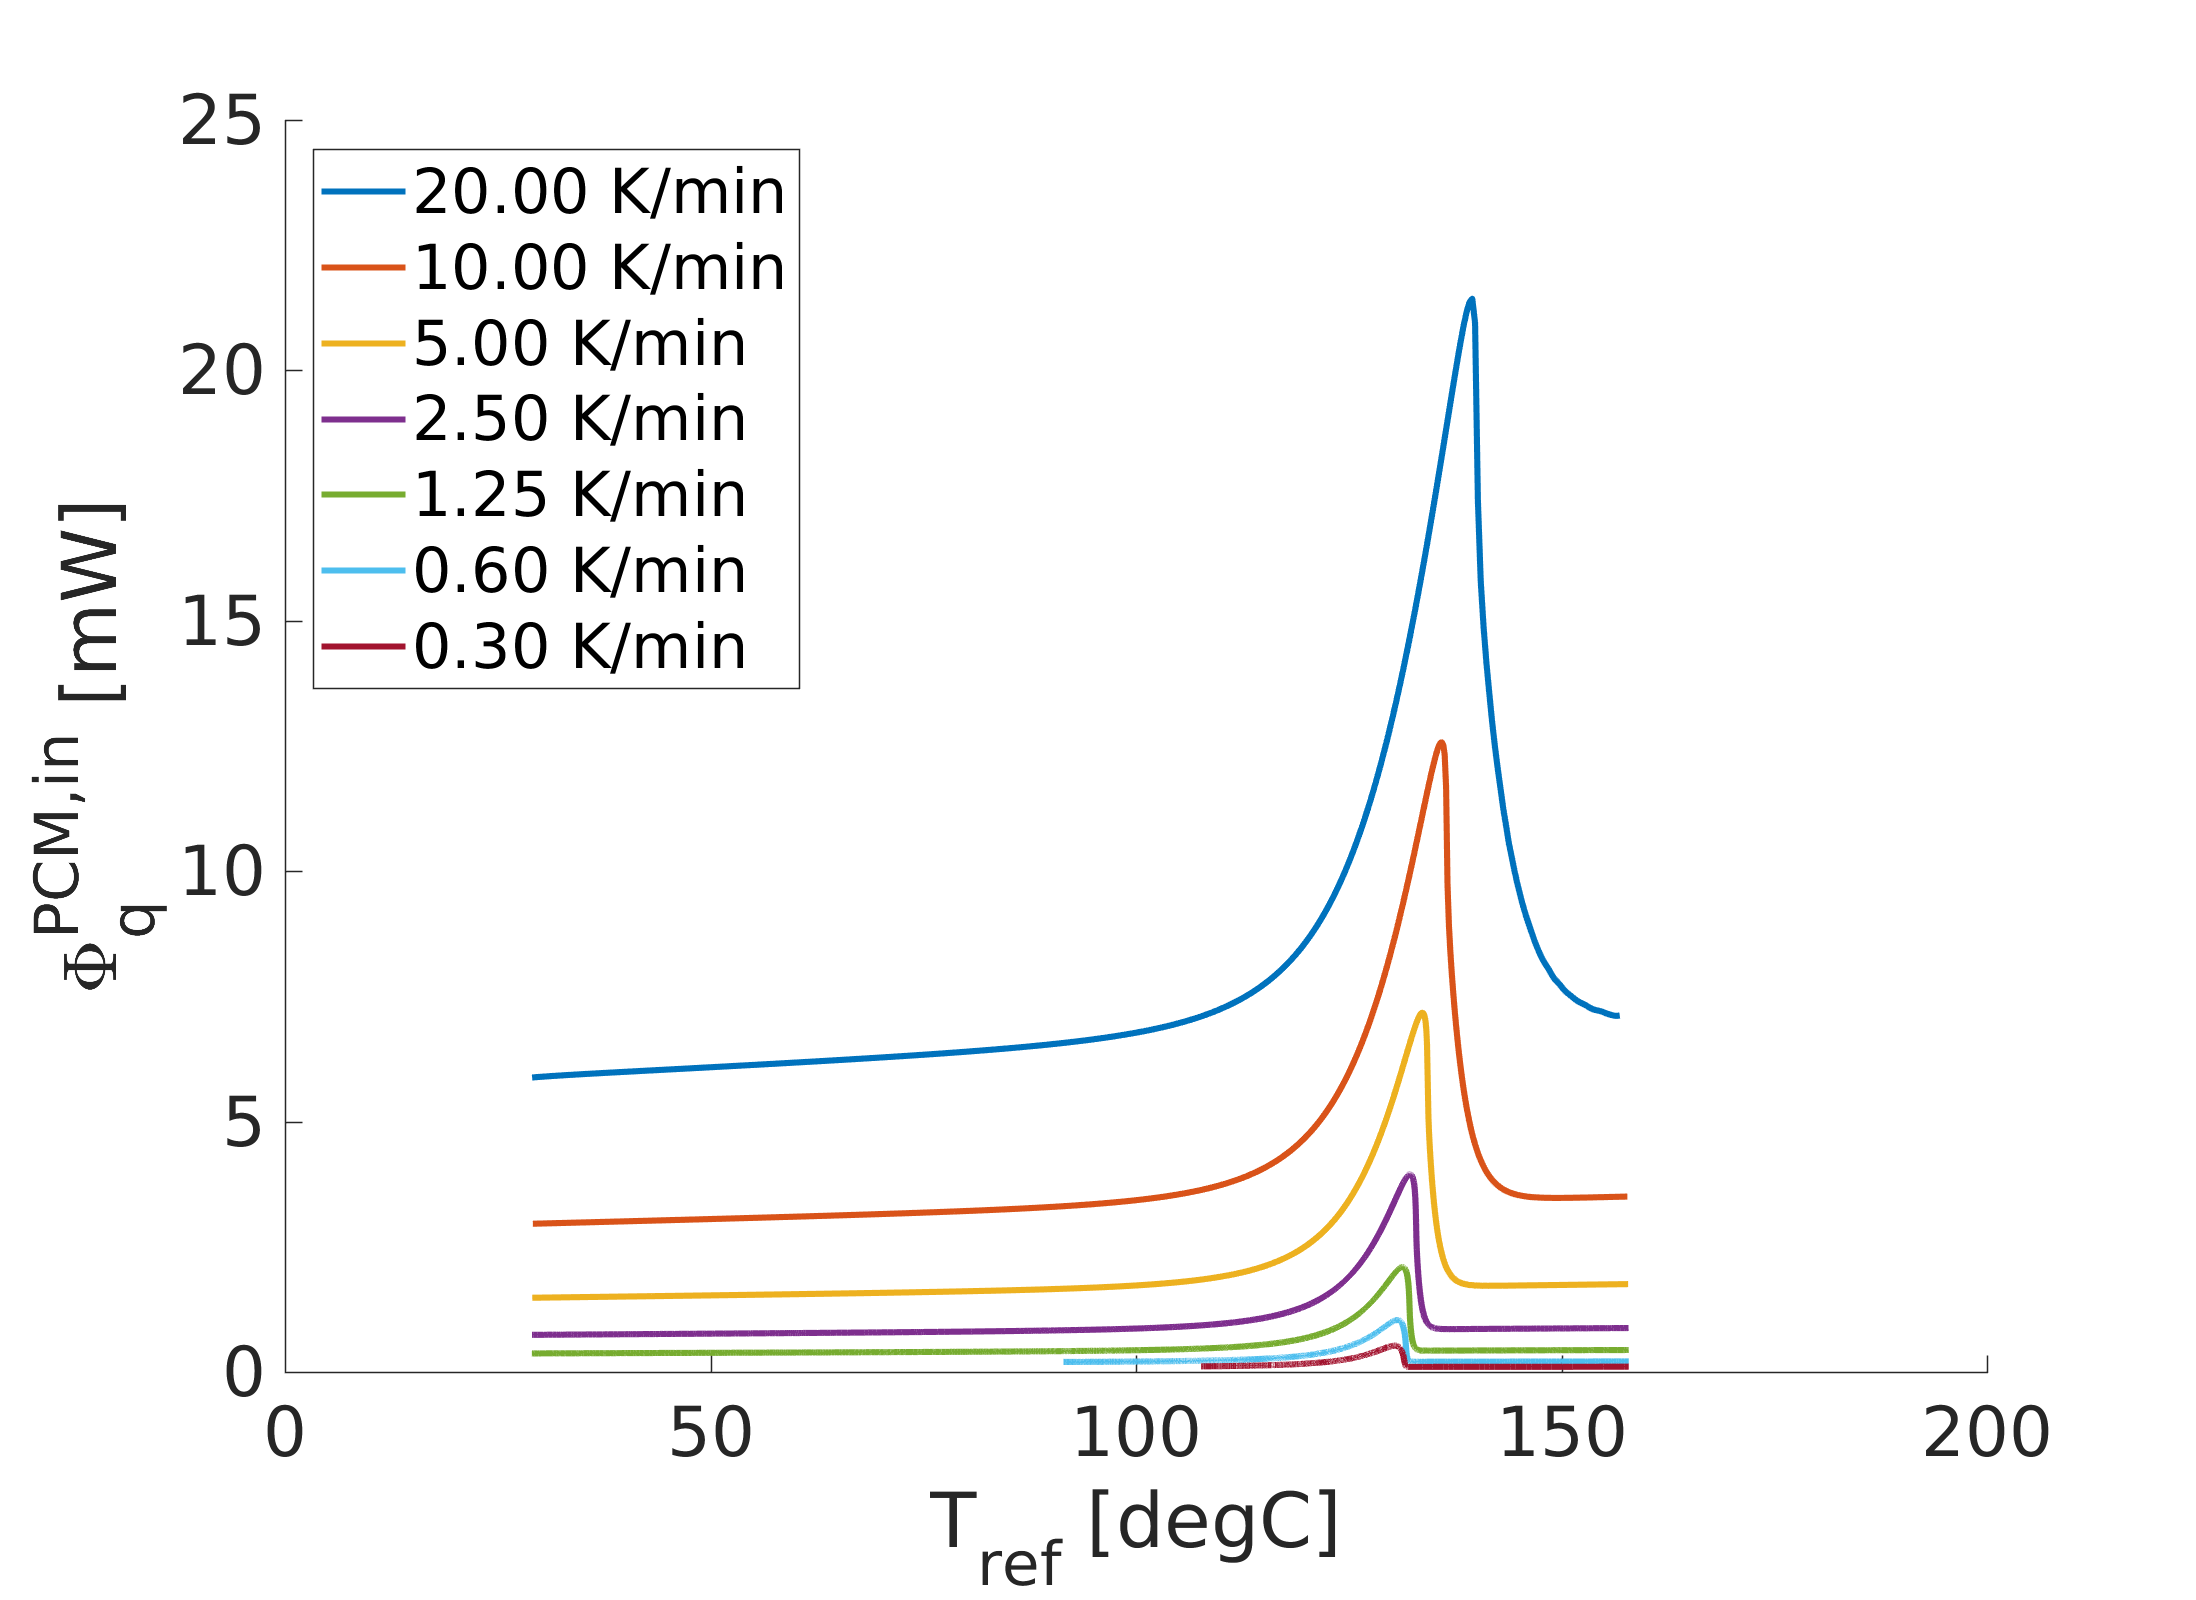
\includegraphics[width=1.\textwidth]{/home/argo/masterarbeit/thesis/images/smearing_effect_simulation_heat_fluxes.png}
		\caption{Heat fluxes from simulation for different heat rates.}
		\label{fig:smearing_effect_simulation_heat_flux}
	\end{subfigure}
	\begin{subfigure}{0.49\textwidth}
		\includegraphics[width=1.\textwidth]{/home/argo/masterarbeit/vortrag/images/heat_flux_measurement.png}
		\caption{Heat flux measurement values for different heat rates.}
		\label{fig:smearing_effect_measurement_heat_flux}
	\end{subfigure}
	\caption{}
\end{figure}



\subsection{Parameter estimation using finite differences and NURBS parametrization}

For the first attempt of estimating $c_p(T)$  we used the NURBS parametrization (see Sec. \ref{sec:nurbs}). In total we used 33 control points where the y-coordinates ($\hat{=} c_p$) are optimization variables and the the x-coordinate ($\hat{=}$ temperature) were fixed to 

\begin{equation}
	P^x = [0, 30, 60, 90, 100, 102, 104, ..., 148, 150, 160, 180, 200]
\end{equation}

such that the peak has enough degrees of freedom for temperatures $T \in [100, 150]$. \\
Due to the early working state we used the matlab routines $ode15s$ for integration and $lsqnonlin$ to solve the least squares problem where the Jacobian was computed via external numerical differentiation. The integration tolerance was set here to $10^{-7}$ as well. Besides that material properties of Constantan were used instead of silver for the heat transport plate from furnace to PCM. In particular these are $c_{p,Const}=0.41\frac{mJ}{mg \ K}$, $\rho_{Const}=10.49\frac{mg}{mm^3}$ and $\lambda_{Const}=23\frac{mW}{mm \ K}$. \\
Minimizing the heat flux residuum worked best in this setting for $L_{Const}=15mm$ (instead of $L_{Ag}$ here) and $L_{pcm}=0.5mm$. \\
The results after optimizing, using the measurement data of heat rate $\beta = 10 \frac{K}{min}$, are shown in Fig. \ref{fig:NURBS_results}. As one can see it was possible to minimize the residuum of heat flux quite well aside from some oscillations which have their origin in $c_p(T)$ due to numerical problems. Beside the oscillations there is one major difference in the peak shape from what we would expect, that is after the peak a temporary decrease followed by a big slope.
Finally $lsqnonlin$ gives us the approximation of the used Jacobian $J_1(p_{c_p})$ at the end of the optimization process which was computed internally via finite differences, see Fig. \ref{fig:NURBS_results}c. Since in our NURBS parametrization the y-coordinates of the control points are free optimization variables and the locality of those the x-axis of these Jacobian plots was set being the x-coordinates of the control points. This way there is a direct connection between $J_1(p_{c_p})$ and which zone of $c_p(T)$ it affects. The y-axis was labeled using the reference crucible temperature since the heat flux measurement values are given as a function of those, analog to the heat flux plot.
Two things are worth mentioning. First the order of magnitude which is increased by several orders for areas of $c_p(T)$ up to temperatures of $100^\circ C$ and measurement values above $110^\circ C$ reference temperature during phase transition. Interestingly the specific heat capacity's oscillations occur in a zone of low sensitivities which explains why $lsqnonlin$ does not improve here further. 
Secondly considering the zone of increased magnitude in detail (see Fig \ref{fig:NURBS_results}d) one recognize sign switching oscillations where continuity is expected. This is a strong indication that the approximation of $J_1(p_{c_p})$ via finite differences is of poor quality and not reliable why we switch to internal numerical differentiation later. \\
The optimization took in this case about 40 minutes on my laptop and stopped because the norm of step was below the tolerance $10^{-6}$.


\begin{figure}[H]
	\subcaptionbox{Heat flux into PCM $\varPhi_q^{pcm,in}$ measurement values (dashed red), simulation (blue) and corresponding residuum (yellow).}[.49\linewidth]
	{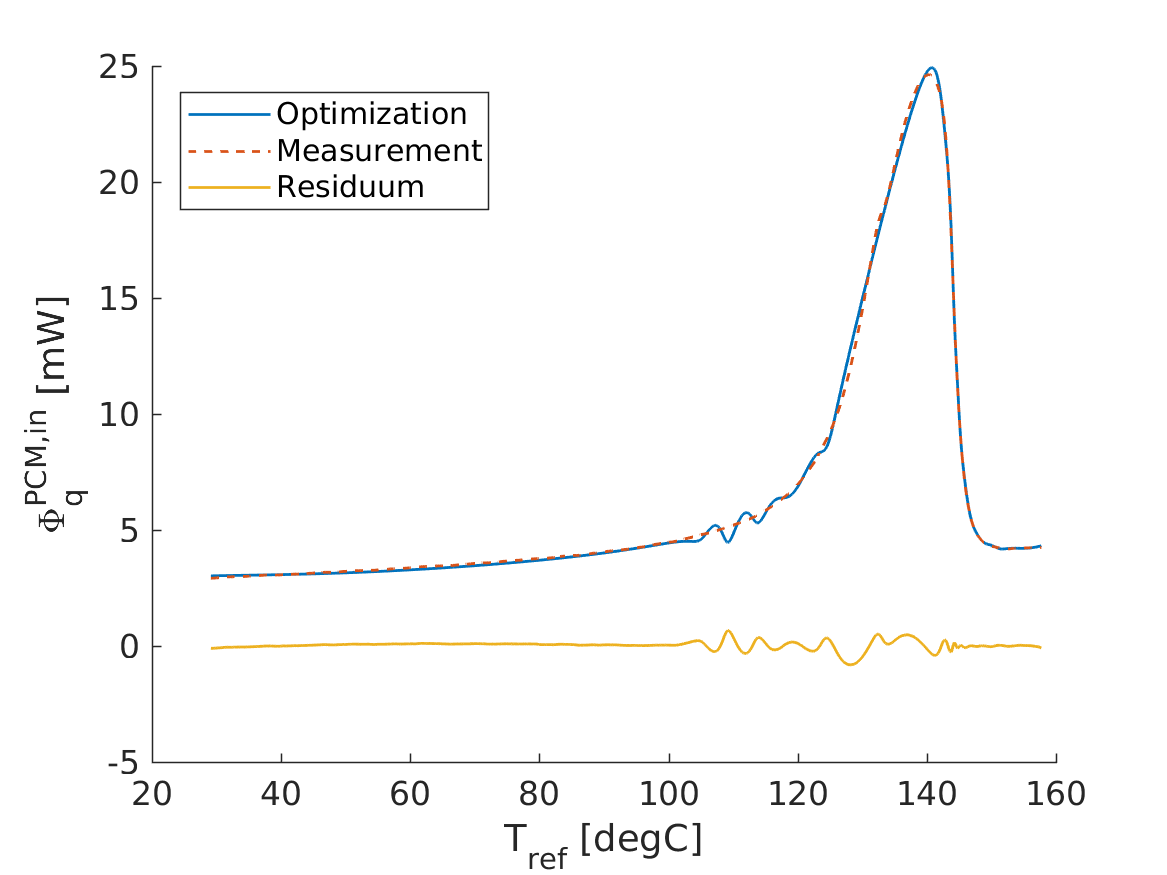
\includegraphics[width=0.49\textwidth]{/home/argo/masterarbeit/thesis/images/NURBS_heat_flux.png}}
	\subcaptionbox{Specific heat capacity $c_p(T)$ obtained by parameter estimation.}[.49\linewidth]
	{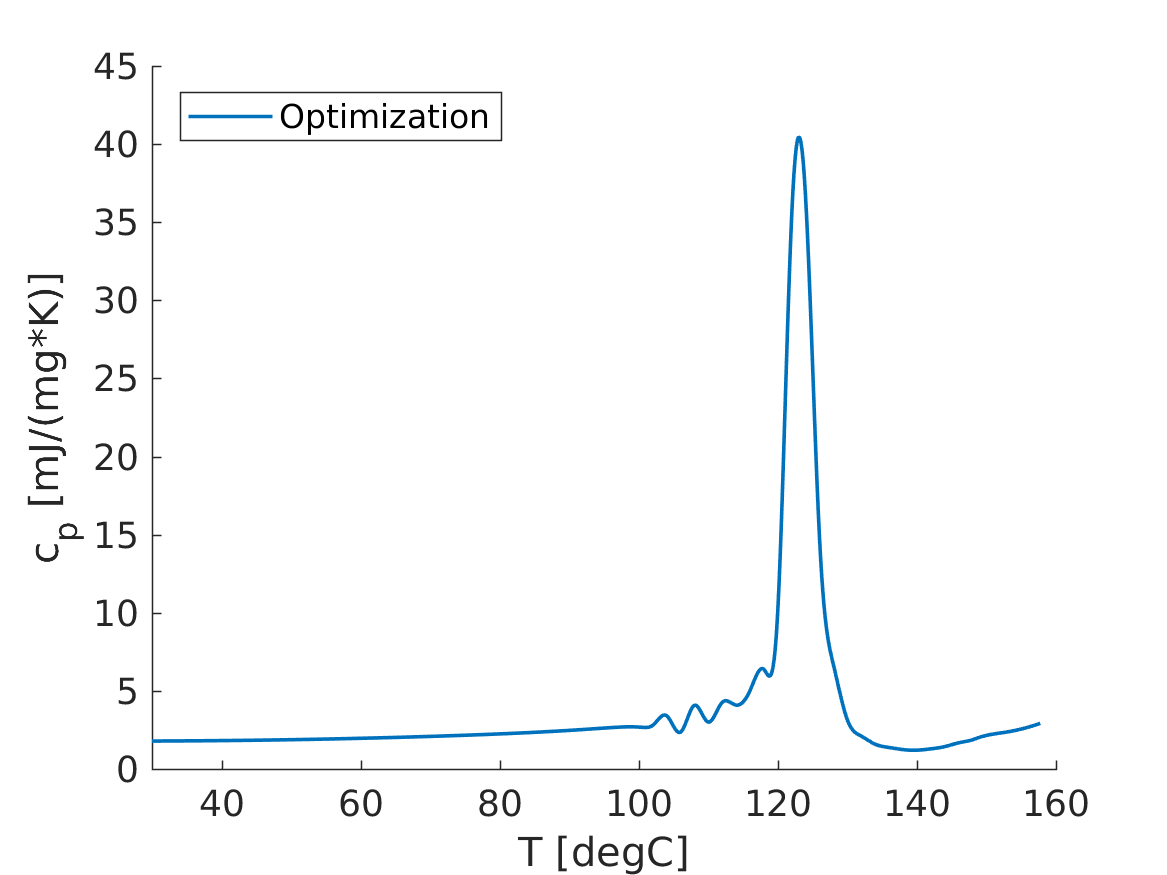
\includegraphics[width=0.49\textwidth]{/home/argo/masterarbeit/thesis/images/NURBS_c_p(T).png}}

	\subcaptionbox{Approximated Jacobian $J_1(p_{c_p})$.}[.49\linewidth]
	{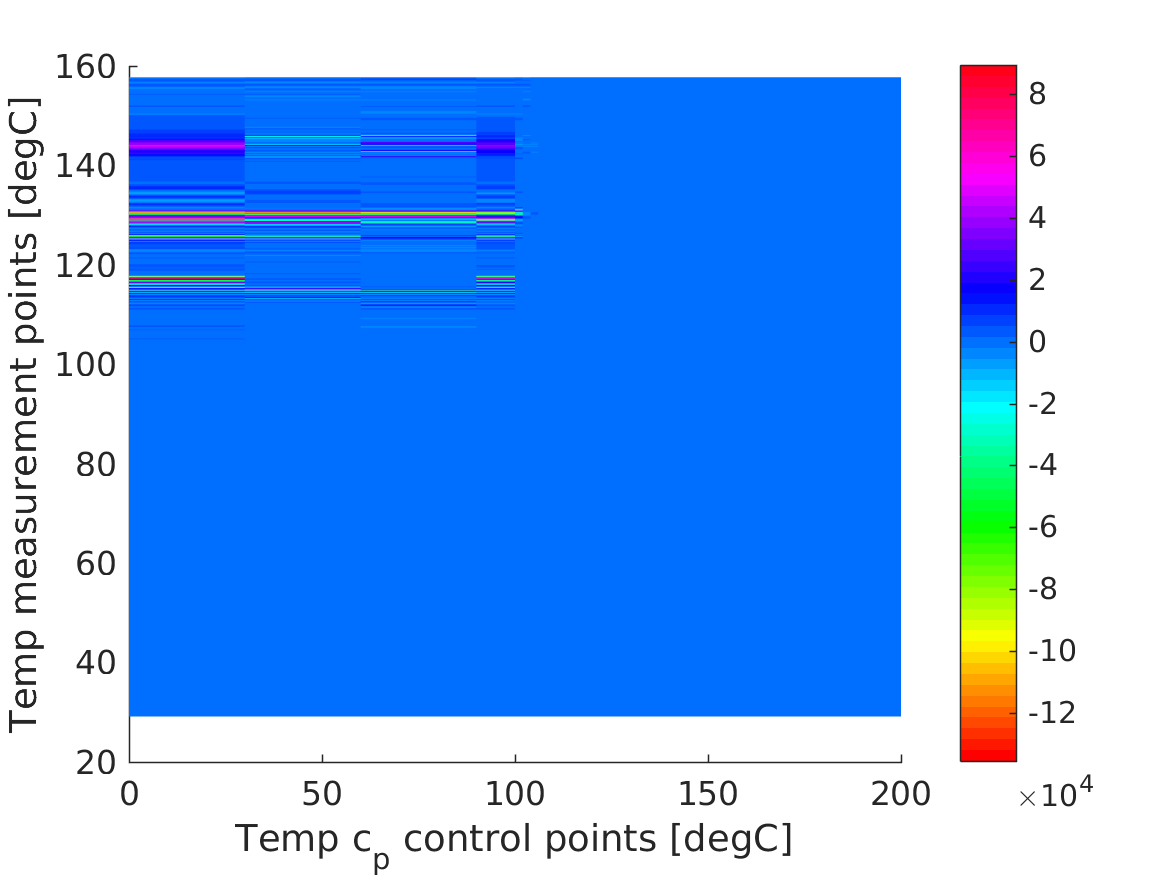
\includegraphics[width=0.49\textwidth]{/home/argo/masterarbeit/thesis/images/NURBS_jac.png}}
	\hspace{0.5cm}
	\subcaptionbox{Zoomed in view of approximated $J_1(p_{c_p})$.}[.49\linewidth]
	{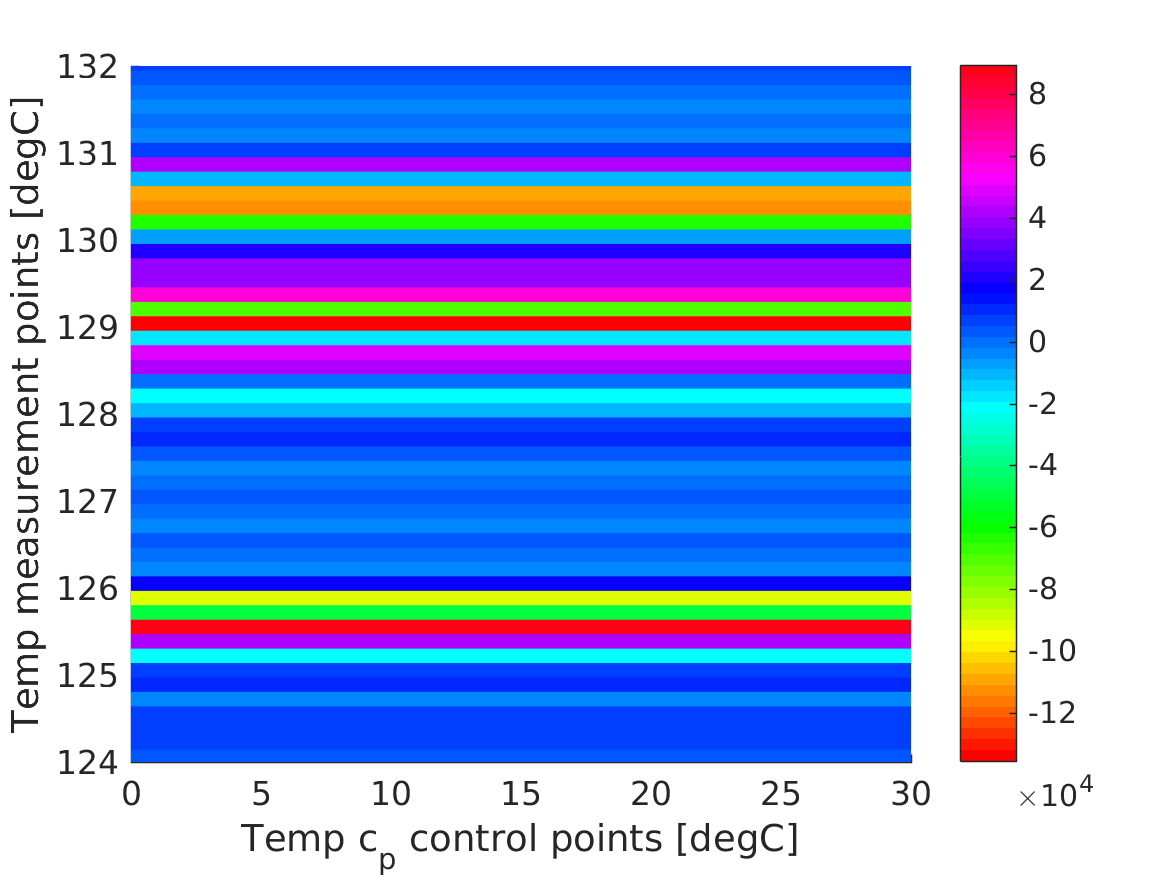
\includegraphics[width=0.49\textwidth]{/home/argo/masterarbeit/thesis/images/NURBS_jac_zoom.png}}
	\caption{Specific heat capacity, heat flux and optimization Jacobian at the end of the optimization process.}
	\label{fig:NURBS_results}
\end{figure}




\subsection{Error analysis of integration tolerance and spatial discretization grid}
In this section we quantify the occurring numerical errors due to the used integration tolerance and spatial discretization grid in order to ensure that these do not influence the results significantly. \\
From here on the numerical integrator DAESOL-II within the SolvIND Suite and the material properties of silver for the silver plate were used for all upcoming numerical experiments. The relative error comparing integration tolerances $10^{-7}$ and $10^{-8}$  is shown in Fig. \ref{fig:integration_tolerance_error}.
The temperature at the last discretization point of the silver plate was evaluated for all measurement time points which equates a temperature at the reference crucible $T_{ref}$. 
As one can see the maximum relative error $1.7 \cdot 10^{-6}$ occurs approximately at the PCM's phase transition. 
From the magnitude we can conclude that a integration tolerance of $10^{-7}$ is sufficient. \\


\begin{figure}[H]
	\centering
	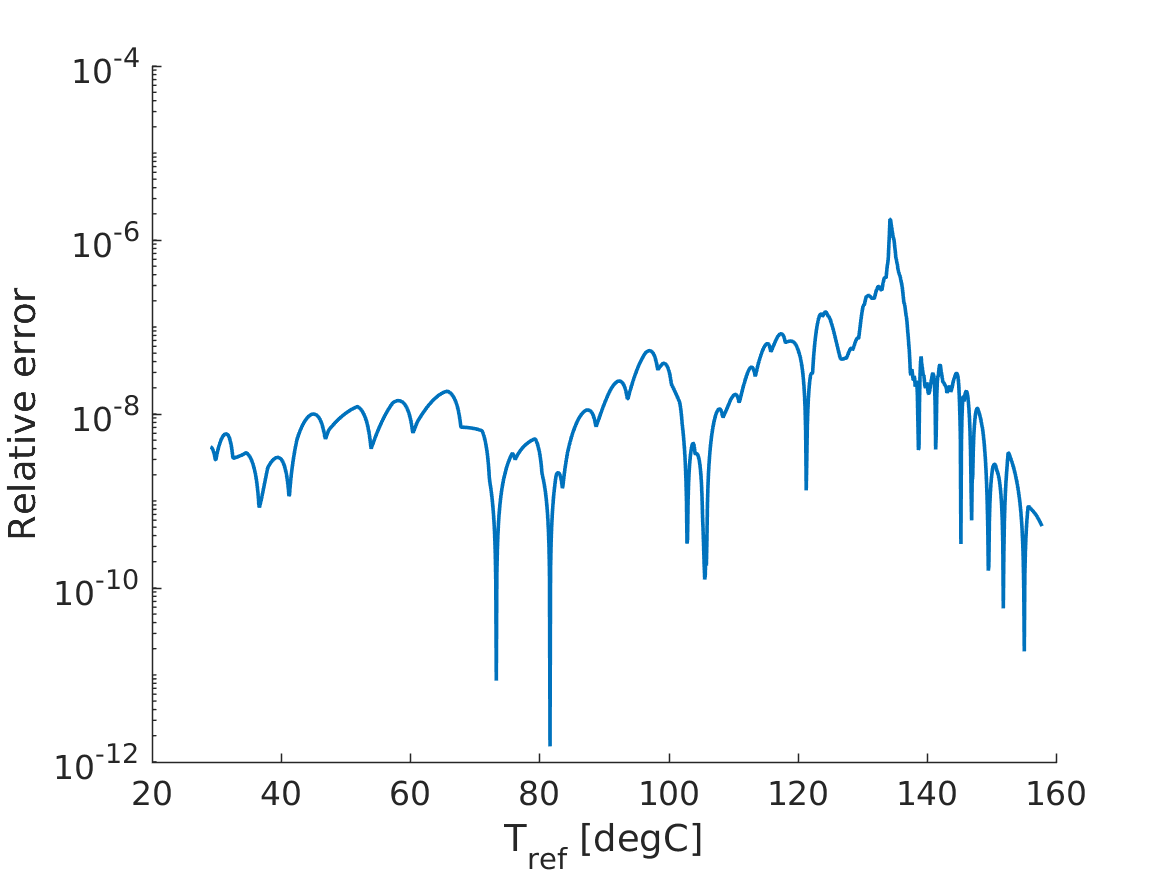
\includegraphics[width=0.75\textwidth]{/home/argo/masterarbeit/thesis/images/integration_tolerance_relErr.png}
	\caption{Computed relative error $|1 - \frac{T^{N_{Ag}-1}_{E_1}}{T^{N_{Ag}-1}_{E_2}}|$ where $T_{E_1}$ used a integration tolerance of $10^{-7}$ and $T_{E_2}$ respectively $10^{-8}$.}
	\label{fig:integration_tolerance_error}
\end{figure}


Next we compare several configurations of the spatial discretization grid (c.f. Sec. \ref{sec:spatial_discretization_grid}) with an equidistant reference grid with $\Delta x = \frac{L_{pcm}}{N_{pcm}}$ everywhere. The used physical lengths $L_{Ag}=40mm$ and $L_{pcm}=0.1mm$ where the optimization worked best together with a sufficiently large number of discretization points within the PCM such that the heat flux approximation is adequate results in a huge number of total discretization points in an equidistant grid. E.g. with $N_{pcm}=50$ the total number of discretization points would be $N=20,050$ which is not practical in the optimization process. Therefore we compute the relative error

\begin{equation}
	| \text{Relative error}_i| = \left| 1 - \frac{T_{{grid}_i}^{N_{Ag}-1}(T_{ref})}{T_{eq}^{N_{Ag}-1}(T_{ref})} \right|
	\label{eq:relErr_grid}
\end{equation}

where $T_{grid_i}^{N_{Ag}-1}$ is the temperature using grid $i$ and $T_{eq}^{N_{Ag}-1}$ is the temperature from the reference equidistant grid using $N_{pcm}=50$ and $N_{Ag}=20,000$. Both temperatures are evaluated at the silver plate's last discretization point since this equates to the same physical coordinate $x=L_{Ag}$ by construction in all grids. 
We set $n_m=0.01$ and $t=0.999$ for all experiments in order to guarantee that the transition of the grid size is finished sufficiently once the PCM starts which is necessary for the heat flux approximation. \\
In the first set of tests we modified the total number of discretization points $N$ while fixing $n_{pcm}=0.2$ and $n_{tr}=0.1$. The results are shown in Fig. \ref{fig:grid_mod_N} where in all upcoming cases (a) shows the grid size $\Delta x = \frac{\partial \chi}{\partial \tilde{x}}(\tilde{x})$ as a function of the computation grid $\tilde{x}$ and (b) maps the corresponding relative error computed by \eqref{eq:relErr_grid}. As one can see in all cases the error increases during the phase transition at a reference crucible temperature of about $130^{\circ} C$ where the maximum is reached for the least amount of tested discretization points $N=200$ with $|\text{Relative error|}=1.5 \cdot 10^{-5}$. Surprisingly the error for $N > 1000$ increases again but in all tested cases the relative error has an order of magnitude lower equal than $10^{-5}$. 


\begin{figure}[H]
	\begin{subfigure}{0.49\textwidth}
		\includegraphics[width=1.\textwidth]{/home/argo/masterarbeit/simulationen-data/grid_error/mod_N_gridsize.png}
		\caption{}
		\label{fig:gridsize_mod_N}
	\end{subfigure}
	\begin{subfigure}{0.49\textwidth}
		\includegraphics[width=1.\textwidth]{/home/argo/masterarbeit/simulationen-data/grid_error/mod_N_relErr.png}
		\caption{}
		\label{fig:grid_relErr_mod_N}
	\end{subfigure}
	\caption{Grid size $\Delta x(\tilde{x}$ (a) and relative error (b) for fixed $n_{tr}=0.1$ and $n_{pcm}=0.2$ while varying total number of discretization points $N$.}
	\label{fig:grid_mod_N}
\end{figure}

Next we varied the number of discretization points in the silver plate while fixing $N_{pcm}=50$ and again $n_{tr}=0.1$. The results are qualitatively and quantitatively similar to the previous case as one can observe in Fig. \ref{fig:grid_mod_N1}.


\begin{figure}[H]
	\begin{subfigure}{0.49\textwidth}
		\includegraphics[width=1.\textwidth]{/home/argo/masterarbeit/simulationen-data/grid_error/mod_N1_gridsize.png}
		\caption{}
		\label{fig:gridsize_mod_N1}
	\end{subfigure}
	\begin{subfigure}{0.49\textwidth}
		\includegraphics[width=1.\textwidth]{/home/argo/masterarbeit/simulationen-data/grid_error/mod_N1_relErr.png}
		\caption{}
		\label{fig:grid_relErr_mod_N1}
	\end{subfigure}
	\caption{Grid size $\Delta x(\tilde{x}$ (a) and relative error (b) for fixed $N_{pcm}=50$ and $N_{tr}=0.1$ while varying discretization points in the silver plate $N_{Ag}$.}
	\label{fig:grid_mod_N1}
\end{figure}


Finally $N_{Ag}=300$ and $N_{pcm}=50$ were fixed while varying the grid transition parameter $n_{tr}$. The relative error increases with increasing $n_{tr}$, i.e. softer transitions. The minimal error is achieved at the phase transition with $n_{tr}=0$ ($\Delta x$ is step function) and else with $n_{tr}=0.1$ while the order of magnitude is again lower equal $10^{-5}$ in these two cases.

\begin{figure}[H]
	\begin{subfigure}{0.49\textwidth}
		\includegraphics[width=1.\textwidth]{/home/argo/masterarbeit/simulationen-data/grid_error/mod_n_tr_gridsize.png}
		\caption{}
		\label{fig:gridsize_mod_n_tr}
	\end{subfigure}
	\begin{subfigure}{0.49\textwidth}
		\includegraphics[width=1.\textwidth]{/home/argo/masterarbeit/simulationen-data/grid_error/mod_n_tr_relErr.png}
		\caption{}
		\label{fig:grid_relErr_mod_n_tr}
	\end{subfigure}
	\caption{Grid size $\Delta x(\tilde{x}$ (a) and relative error (b) for fixed $N_{Ag}=300$ and $N_{pcm}=50$ while varying the grid transition parameter $n_{tr}$.}
	\label{fig:grid_mod_n_tr}
\end{figure}

Summarized a total number of discretization points $N=300$ is sufficient while the transition parameter $n_{tr}$ should not be much larger than $0.1$. Then the magnitude of the relative error is lower equal $10^{-5}$ which is negligible especially when considering that the relative integration tolerance $10^{-7}$ was used.




\subsection{Parameter estimation using parametrization of linear combination of Gaussians}

%\begin{figure}[H]
%		\begin{subfigure}{0.32\textwidth}
%			\includegraphics[width=1.\textwidth]{/home/argo/masterarbeit/fits_data/2017-12-08_22:22:31_407_L1=40_L3=0,1_N1=300_N3=50_5Gaussians/2017-12-08_22:31:48_407_20Kmin_L1=40_L3=0,1/combined_img.png}
%			\caption{$\beta = 20 \frac{K}{min}$}
%		\end{subfigure}
%		\begin{subfigure}{0.32\textwidth}
%			\includegraphics[width=1.\textwidth]{/home/argo/masterarbeit/fits_data/2017-12-08_22:22:31_407_L1=40_L3=0,1_N1=300_N3=50_5Gaussians/2017-12-08_22:39:19_407_10Kmin_L1=40_L3=0,1/combined_img.png}
%			\caption{$\beta = 10 \frac{K}{min}$}
%		\end{subfigure}
%		\begin{subfigure}{0.32\textwidth}
%			\includegraphics[width=1.\textwidth]{/home/argo/masterarbeit/fits_data/2017-12-08_22:22:31_407_L1=40_L3=0,1_N1=300_N3=50_5Gaussians/2017-12-08_22:53:51_407_5Kmin_L1=40_L3=0,1/combined_img.png}
%			\caption{$\beta = 5 \frac{K}{min}$}
%		\end{subfigure}
%		\begin{subfigure}{0.32\textwidth}
%			\includegraphics[width=1.\textwidth]{/home/argo/masterarbeit/fits_data/2017-12-08_22:22:31_407_L1=40_L3=0,1_N1=300_N3=50_5Gaussians/2017-12-08_22:59:44_407_2,5Kmin_L1=40_L3=0,1/combined_img.png}
%			\caption{$\beta = 2.5 \frac{K}{min}$}
%		\end{subfigure}
%		\begin{subfigure}{0.32\textwidth}
%			\includegraphics[width=1.\textwidth]{/home/argo/masterarbeit/fits_data/2017-12-08_22:22:31_407_L1=40_L3=0,1_N1=300_N3=50_5Gaussians/2017-12-08_23:42:17_407_1,25Kmin_L1=40_L3=0,1/combined_img.png}
%			\caption{$\beta = 1.25 \frac{K}{min}$}
%		\end{subfigure}
%		\begin{subfigure}{0.32\textwidth}
%			\includegraphics[width=1.\textwidth]{/home/argo/masterarbeit/fits_data/2017-12-08_22:22:31_407_L1=40_L3=0,1_N1=300_N3=50_5Gaussians/2017-12-08_23:47:19_407_0,6Kmin_L1=40_L3=0,1/combined_img.png}
%			\caption{$\beta = 0.6 \frac{K}{min}$}
%		\end{subfigure}
%		\centering
%		\begin{subfigure}{0.32\textwidth}
%			\includegraphics[width=1.\textwidth]{/home/argo/masterarbeit/fits_data/2017-12-08_22:22:31_407_L1=40_L3=0,1_N1=300_N3=50_5Gaussians/2017-12-08_23:53:54_407_0,3Kmin_L1=40_L3=0,1/combined_img.png}
%			\caption{$\beta = 0.3 \frac{K}{min}$}
%		\end{subfigure}
%		\caption{}
%		\label{fig:5Gaussians_c_p_heat_flux_combo}
%\end{figure}




\begin{figure}[H]
	\begin{subfigure}{1.\textwidth}
		\includegraphics[width=0.49\textwidth]{/home/argo/masterarbeit/fits_data/2017-12-08_22:22:31_407_L1=40_L3=0,1_N1=300_N3=50_5Gaussians/2017-12-08_22:31:48_407_20Kmin_L1=40_L3=0,1/c_p.png}
		\includegraphics[width=0.49\textwidth]{/home/argo/masterarbeit/fits_data/2017-12-08_22:22:31_407_L1=40_L3=0,1_N1=300_N3=50_5Gaussians/2017-12-08_22:31:48_407_20Kmin_L1=40_L3=0,1/heat_flux.png}
	\end{subfigure} \\[1ex]
	
	\begin{subfigure}{1.\textwidth}
		\includegraphics[width=0.49\textwidth]{/home/argo/masterarbeit/fits_data/2017-12-08_22:22:31_407_L1=40_L3=0,1_N1=300_N3=50_5Gaussians/2017-12-08_22:39:19_407_10Kmin_L1=40_L3=0,1/c_p.png}
		\includegraphics[width=0.49\textwidth]{/home/argo/masterarbeit/fits_data/2017-12-08_22:22:31_407_L1=40_L3=0,1_N1=300_N3=50_5Gaussians/2017-12-08_22:39:19_407_10Kmin_L1=40_L3=0,1/heat_flux.png}
	\end{subfigure} \\[1ex]
	
	\begin{subfigure}{1.\textwidth}
		\includegraphics[width=0.49\textwidth]{/home/argo/masterarbeit/fits_data/2017-12-08_22:22:31_407_L1=40_L3=0,1_N1=300_N3=50_5Gaussians/2017-12-08_22:53:51_407_5Kmin_L1=40_L3=0,1/c_p.png}
		\includegraphics[width=0.49\textwidth]{/home/argo/masterarbeit/fits_data/2017-12-08_22:22:31_407_L1=40_L3=0,1_N1=300_N3=50_5Gaussians/2017-12-08_22:53:51_407_5Kmin_L1=40_L3=0,1/heat_flux.png}
	\end{subfigure} \\[1ex]
	
	\begin{subfigure}{1.\textwidth}
		\includegraphics[width=0.49\textwidth]{/home/argo/masterarbeit/fits_data/2017-12-08_22:22:31_407_L1=40_L3=0,1_N1=300_N3=50_5Gaussians/2017-12-08_22:59:44_407_2,5Kmin_L1=40_L3=0,1/c_p.png}
		\includegraphics[width=0.49\textwidth]{/home/argo/masterarbeit/fits_data/2017-12-08_22:22:31_407_L1=40_L3=0,1_N1=300_N3=50_5Gaussians/2017-12-08_22:59:44_407_2,5Kmin_L1=40_L3=0,1/heat_flux.png}
	\end{subfigure} \\[1ex]
	\caption{}
	\label{fig:optim_c_p_heat_flux_5Gaussians_1}
\end{figure}


\begin{figure}[H]
	\begin{subfigure}{1.\textwidth}
		\includegraphics[width=0.49\textwidth]{/home/argo/masterarbeit/fits_data/2017-12-08_22:22:31_407_L1=40_L3=0,1_N1=300_N3=50_5Gaussians/2017-12-08_23:42:17_407_1,25Kmin_L1=40_L3=0,1/c_p.png}
		\includegraphics[width=0.49\textwidth]{/home/argo/masterarbeit/fits_data/2017-12-08_22:22:31_407_L1=40_L3=0,1_N1=300_N3=50_5Gaussians/2017-12-08_23:42:17_407_1,25Kmin_L1=40_L3=0,1/heat_flux.png}
	\end{subfigure} \\[1ex]
	
	\begin{subfigure}{1.\textwidth}
		\includegraphics[width=0.49\textwidth]{/home/argo/masterarbeit/fits_data/2017-12-08_22:22:31_407_L1=40_L3=0,1_N1=300_N3=50_5Gaussians/2017-12-08_23:47:19_407_0,6Kmin_L1=40_L3=0,1/c_p.png}
		\includegraphics[width=0.49\textwidth]{/home/argo/masterarbeit/fits_data/2017-12-08_22:22:31_407_L1=40_L3=0,1_N1=300_N3=50_5Gaussians/2017-12-08_23:47:19_407_0,6Kmin_L1=40_L3=0,1/heat_flux.png}
	\end{subfigure} \\[1ex]
	
	\begin{subfigure}{1.\textwidth}
		\includegraphics[width=0.49\textwidth]{/home/argo/masterarbeit/fits_data/2017-12-08_22:22:31_407_L1=40_L3=0,1_N1=300_N3=50_5Gaussians/2017-12-08_23:53:54_407_0,3Kmin_L1=40_L3=0,1/c_p.png}
		\includegraphics[width=0.49\textwidth]{/home/argo/masterarbeit/fits_data/2017-12-08_22:22:31_407_L1=40_L3=0,1_N1=300_N3=50_5Gaussians/2017-12-08_23:53:54_407_0,3Kmin_L1=40_L3=0,1/heat_flux.png}
	\end{subfigure} \\[1ex]
	\caption{}
	\label{fig:optim_c_p_heat_flux_5Gaussians_2}
\end{figure}




\begin{table}[H]
	\centering
	\begin{tabular}{| c | c | c | c | c | c | c | c | c |} \hline
		Heat rate $\beta$ & Gauss1 & Gauss2 & Gauss3 & Gauss4 & Gauss5 & Linear & Const & $||\nabla \mathcal{L}||_2$ \\ 
		$[K/min]$ & & & & & & & & \\ \hline
		$20$ & & & & & & & & \\
		$10$ & & & & & & & & \\
		$5$ & & & & & & & & \\
		$2.5$ & & & & & & & & \\
		$1.25$ & & & & & & & & \\
		$0.6$ & & & & & & & & \\
		$0.3$ & & & & & & & & \\ \hline
	\end{tabular}
	\caption{}
	\label{tab:parameter_table_5Gaussians}
\end{table}

\begin{table}[H]
	\centering
	\begin{tabular}{| c | c | c | c | c | c | c | c |} \hline
		Heat rate $\beta$ & 20 & 10 & 5 & 2.5 & 1.25 & 0.6 & 0.3 \\
		$[K/min]$ & & & & & & & \\ \hline
		$T_{max} \ [^{\circ}C]$ & $126.3$ & ---$^*$ & $126.9$ & $127.9$ & $128.9$ & $129.8$ & $130.5$ \\
		$\Delta H \ [\frac{mJ}{mg}]$ & $162.8$ & $187.6$ & $211.6$ & $211.5$ & $208.8$ & $195.5$ & $191.1$ \\ \hline
	\end{tabular}
	\caption{\todo{$^*$ erklaeren}}
	\label{fig:eval_table_Tmax_deltaH_5Gaussians}
\end{table}

\todo{Auswertung Mittelwert + Standardabweichung der Peakposition}

\begin{figure}[H]
	\centering
	\includegraphics[width=0.8\textwidth]{/home/argo/masterarbeit/fits_data/2017-12-08_22:22:31_407_L1=40_L3=0,1_N1=300_N3=50_5Gaussians/c_p_all.png}
	\caption{}
	\label{fig:5Gaussians_all_c_p}
\end{figure}


\todo{Optimierungsdauer}


\subsection{Parameter estimation using Fraser-Suzuki parametrization}
\label{sec:param_estimation_fs}



%\begin{figure}[H]
%	\begin{subfigure}{0.32\textwidth}
%		\includegraphics[width=1.\textwidth]{/home/argo/masterarbeit/fits_data/2017-12-09_18:33:20_407_L1=40_L3=0,1_N1=300_N3=50_GN_FS/2017-12-09_18:37:41_407_20Kmin_L1=40_L3=0,1/combined_img.png}
%		\caption{$\beta = 20 \frac{K}{min}$}
%	\end{subfigure}
%	\begin{subfigure}{0.32\textwidth}
%		\includegraphics[width=1.\textwidth]{/home/argo/masterarbeit/fits_data/2017-12-09_18:33:20_407_L1=40_L3=0,1_N1=300_N3=50_GN_FS/2017-12-09_18:40:03_407_10Kmin_L1=40_L3=0,1/combined_img.png}
%		\caption{$\beta = 10 \frac{K}{min}$}
%	\end{subfigure}
%	\begin{subfigure}{0.32\textwidth}
%		\includegraphics[width=1.\textwidth]{/home/argo/masterarbeit/fits_data/2017-12-09_18:33:20_407_L1=40_L3=0,1_N1=300_N3=50_GN_FS/2017-12-09_18:43:30_407_5Kmin_L1=40_L3=0,1/combined_img.png}
%		\caption{$\beta = 5 \frac{K}{min}$}
%	\end{subfigure}
%	\begin{subfigure}{0.32\textwidth}
%		\includegraphics[width=1.\textwidth]{/home/argo/masterarbeit/fits_data/2017-12-09_18:33:20_407_L1=40_L3=0,1_N1=300_N3=50_GN_FS/2017-12-09_18:45:47_407_2,5Kmin_L1=40_L3=0,1/combined_img.png}
%		\caption{$\beta = 2.5 \frac{K}{min}$}
%	\end{subfigure}
%	\begin{subfigure}{0.32\textwidth}
%		\includegraphics[width=1.\textwidth]{/home/argo/masterarbeit/fits_data/2017-12-09_18:33:20_407_L1=40_L3=0,1_N1=300_N3=50_GN_FS/2017-12-09_18:48:35_407_1,25Kmin_L1=40_L3=0,1/combined_img.png}
%		\caption{$\beta = 1.25 \frac{K}{min}$}
%	\end{subfigure}
%	\begin{subfigure}{0.32\textwidth}
%		\includegraphics[width=1.\textwidth]{/home/argo/masterarbeit/fits_data/2017-12-09_18:33:20_407_L1=40_L3=0,1_N1=300_N3=50_GN_FS/2017-12-09_18:52:16_407_0,6Kmin_L1=40_L3=0,1/combined_img.png}
%		\caption{$\beta = 0.6 \frac{K}{min}$}
%	\end{subfigure}
%	\centering
%	\begin{subfigure}{0.32\textwidth}
%		\includegraphics[width=1.\textwidth]{/home/argo/masterarbeit/fits_data/2017-12-09_18:33:20_407_L1=40_L3=0,1_N1=300_N3=50_GN_FS/2017-12-09_18:56:18_407_0,3Kmin_L1=40_L3=0,1/combined_img.png}
%		\caption{$\beta = 0.3 \frac{K}{min}$}
%	\end{subfigure}
%	\caption{}
%	\label{fig:FS_c_p_heat_flux_combo}
%\end{figure}



\begin{figure}[H]
	\begin{subfigure}{1.\textwidth}
		\includegraphics[width=0.49\textwidth]{/home/argo/masterarbeit/fits_data/2017-12-09_18:33:20_407_L1=40_L3=0,1_N1=300_N3=50_GN_FS/2017-12-09_18:37:41_407_20Kmin_L1=40_L3=0,1/c_p.png}
		\includegraphics[width=0.49\textwidth]{/home/argo/masterarbeit/fits_data/2017-12-09_18:33:20_407_L1=40_L3=0,1_N1=300_N3=50_GN_FS/2017-12-09_18:37:41_407_20Kmin_L1=40_L3=0,1/heat_flux.png}
	\end{subfigure} \\[1ex]
	
	\begin{subfigure}{1.\textwidth}
		\includegraphics[width=0.49\textwidth]{/home/argo/masterarbeit/fits_data/2017-12-09_18:33:20_407_L1=40_L3=0,1_N1=300_N3=50_GN_FS/2017-12-09_18:40:03_407_10Kmin_L1=40_L3=0,1/c_p.png}
		\includegraphics[width=0.49\textwidth]{/home/argo/masterarbeit/fits_data/2017-12-09_18:33:20_407_L1=40_L3=0,1_N1=300_N3=50_GN_FS/2017-12-09_18:40:03_407_10Kmin_L1=40_L3=0,1/heat_flux.png}
	\end{subfigure} \\[1ex]
	
	\begin{subfigure}{1.\textwidth}
		\includegraphics[width=0.49\textwidth]{/home/argo/masterarbeit/fits_data/2017-12-09_18:33:20_407_L1=40_L3=0,1_N1=300_N3=50_GN_FS/2017-12-09_18:43:30_407_5Kmin_L1=40_L3=0,1/c_p.png}
		\includegraphics[width=0.49\textwidth]{/home/argo/masterarbeit/fits_data/2017-12-09_18:33:20_407_L1=40_L3=0,1_N1=300_N3=50_GN_FS/2017-12-09_18:43:30_407_5Kmin_L1=40_L3=0,1/heat_flux.png}
	\end{subfigure} \\[1ex]
	
	\begin{subfigure}{1.\textwidth}
		\includegraphics[width=0.49\textwidth]{/home/argo/masterarbeit/fits_data/2017-12-09_18:33:20_407_L1=40_L3=0,1_N1=300_N3=50_GN_FS/2017-12-09_18:45:47_407_2,5Kmin_L1=40_L3=0,1/c_p.png}
		\includegraphics[width=0.49\textwidth]{/home/argo/masterarbeit/fits_data/2017-12-09_18:33:20_407_L1=40_L3=0,1_N1=300_N3=50_GN_FS/2017-12-09_18:45:47_407_2,5Kmin_L1=40_L3=0,1/heat_flux.png}
	\end{subfigure}
	\caption{}
	\label{fig:optim_c_p_heat_flux_FS_1}
\end{figure}


\begin{figure}[H]
	\begin{subfigure}{1.\textwidth}
		\includegraphics[width=0.49\textwidth]{/home/argo/masterarbeit/fits_data/2017-12-09_18:33:20_407_L1=40_L3=0,1_N1=300_N3=50_GN_FS/2017-12-09_18:48:35_407_1,25Kmin_L1=40_L3=0,1/c_p.png}
		\includegraphics[width=0.49\textwidth]{/home/argo/masterarbeit/fits_data/2017-12-09_18:33:20_407_L1=40_L3=0,1_N1=300_N3=50_GN_FS/2017-12-09_18:48:35_407_1,25Kmin_L1=40_L3=0,1/heat_flux.png}
	\end{subfigure} \\[1ex]
	
	\begin{subfigure}{1.\textwidth}
		\includegraphics[width=0.49\textwidth]{/home/argo/masterarbeit/fits_data/2017-12-09_18:33:20_407_L1=40_L3=0,1_N1=300_N3=50_GN_FS/2017-12-09_18:52:16_407_0,6Kmin_L1=40_L3=0,1/c_p.png}
		\includegraphics[width=0.49\textwidth]{/home/argo/masterarbeit/fits_data/2017-12-09_18:33:20_407_L1=40_L3=0,1_N1=300_N3=50_GN_FS/2017-12-09_18:52:16_407_0,6Kmin_L1=40_L3=0,1/heat_flux.png}
	\end{subfigure} \\[1ex]
	
	\begin{subfigure}{1.\textwidth}
		\includegraphics[width=0.49\textwidth]{/home/argo/masterarbeit/fits_data/2017-12-09_18:33:20_407_L1=40_L3=0,1_N1=300_N3=50_GN_FS/2017-12-09_18:56:18_407_0,3Kmin_L1=40_L3=0,1/c_p.png}
		\includegraphics[width=0.49\textwidth]{/home/argo/masterarbeit/fits_data/2017-12-09_18:33:20_407_L1=40_L3=0,1_N1=300_N3=50_GN_FS/2017-12-09_18:56:18_407_0,3Kmin_L1=40_L3=0,1/heat_flux.png}
	\end{subfigure}
	\caption{}
	\label{fig:optim_c_p_heat_flux_FS_2}
\end{figure}




\begin{table}[H]
	\centering
	\begin{tabular}{| c | c | c | c | c | c | c |} \hline
		Heat rate $\beta$ & $h$ & $wr$ & $sr$ & $z$ & Linear & Const \\ 
		$[K/min]$ & & & & & & \\ \hline
		$20$ & & & & & & \\
		$10$ & & & & & &  \\
		$5$ & & & & & & \\
		$2.5$ & & & & & & \\
		$1.25$ & & & & & & \\
		$0.6$ & & & & & & \\
		$0.3$ & & & & & & \\ \hline
	\end{tabular}
	\caption{}
	\label{tab:parameter_table_FS}
\end{table}

\begin{table}[H]
	\centering
	\begin{tabular}{| c | c | c | c | c | c | c | c |} \hline
		Heat rate $\beta$ & 20 & 10 & 5 & 2.5 & 1.25 & 0.6 & 0.3 \\
		$[K/min]$ & & & & & & & \\ \hline
		$T_{max} \ [^{\circ}C]$ & $129.0$ & $130.0$ & $128.6$ & $128.8$ & $129.4$ & $130.1$ & $130.7$ \\
		$\Delta H \ [mJ]$ & $162.7$ & $197.0$ & $184.3$ & $176.6$ & $173.1$ & $171.5$ & $172.2$ \\ \hline
	\end{tabular}
	\caption{}
	\label{fig:eval_table_Tmax_deltaH_FS}
\end{table}

\todo{Stat. Parameter aller Werte: $T_{max} = 129.51 \pm 0.78$, hier Standardabweichung}


\begin{figure}[H]
	\centering
	\includegraphics[width=0.8\textwidth]{/home/argo/masterarbeit/fits_data/2017-12-09_18:33:20_407_L1=40_L3=0,1_N1=300_N3=50_GN_FS/c_p_all.png}
	\caption{}
	\label{fig:FS_all_c_p}
\end{figure}




\begin{figure}[H]
	\begin{subfigure}{0.32\textwidth}
		\includegraphics[width=1.\textwidth]{/home/argo/masterarbeit/fits_data/2017-12-10_14:33:40_407_L1=40_L3=0,1_N1=300_N3=50_GN_FS/2017-12-10_14:36:10_407_20Kmin_L1=40_L3=0,1/optimization_progress.png}
		\caption{$\beta = 20 \frac{K}{min}$}
	\end{subfigure}
	\begin{subfigure}{0.32\textwidth}
		\includegraphics[width=1.\textwidth]{/home/argo/masterarbeit/fits_data/2017-12-10_14:33:40_407_L1=40_L3=0,1_N1=300_N3=50_GN_FS/2017-12-10_14:38:49_407_10Kmin_L1=40_L3=0,1/optimization_progress.png}
		\caption{$\beta = 10 \frac{K}{min}$}
	\end{subfigure}
	\begin{subfigure}{0.32\textwidth}
		\includegraphics[width=1.\textwidth]{/home/argo/masterarbeit/fits_data/2017-12-10_14:33:40_407_L1=40_L3=0,1_N1=300_N3=50_GN_FS/2017-12-10_14:41:20_407_5Kmin_L1=40_L3=0,1/optimization_progress.png}
		\caption{$\beta = 5 \frac{K}{min}$}
	\end{subfigure}
	\begin{subfigure}{0.32\textwidth}
		\includegraphics[width=1.\textwidth]{/home/argo/masterarbeit/fits_data/2017-12-10_14:33:40_407_L1=40_L3=0,1_N1=300_N3=50_GN_FS/2017-12-10_14:44:26_407_2,5Kmin_L1=40_L3=0,1/optimization_progress.png}
		\caption{$\beta = 2.5 \frac{K}{min}$}
	\end{subfigure}
	\begin{subfigure}{0.32\textwidth}
		\includegraphics[width=1.\textwidth]{/home/argo/masterarbeit/fits_data/2017-12-10_14:33:40_407_L1=40_L3=0,1_N1=300_N3=50_GN_FS/2017-12-10_14:47:00_407_1,25Kmin_L1=40_L3=0,1/optimization_progress.png}
		\caption{$\beta = 1.25 \frac{K}{min}$}
	\end{subfigure}
	\begin{subfigure}{0.32\textwidth}
		\includegraphics[width=1.\textwidth]{/home/argo/masterarbeit/fits_data/2017-12-10_14:33:40_407_L1=40_L3=0,1_N1=300_N3=50_GN_FS/2017-12-10_14:49:40_407_0,6Kmin_L1=40_L3=0,1/optimization_progress.png}
		\caption{$\beta = 0.6 \frac{K}{min}$}
	\end{subfigure}
	\begin{subfigure}{0.32\textwidth}
		\includegraphics[width=1.\textwidth]{/home/argo/masterarbeit/fits_data/2017-12-10_14:33:40_407_L1=40_L3=0,1_N1=300_N3=50_GN_FS/2017-12-10_14:53:25_407_0,3Kmin_L1=40_L3=0,1/optimization_progress.png}
		\caption{$\beta = 0.6 \frac{K}{min}$}
	\end{subfigure}
	\caption{}
	\label{fig:optimization_progress_FS}
\end{figure}


\todo{Optimierungsdauer}


\subsection{Parameter estimation with modified heat rate from measurement data}
So far just the nominal heat rate of the appropriate measurement scheme was used. 
Fig. \ref{fig:heat_rate_measurement} shows the measurement data of the heat rate at the reference crucible $\frac{\partial T_{ref}(t)}{\partial t}(T_{ref})$ exemplary for a nominal heat rate $\beta = 2.5 \frac{K}{min}$. 
As one can see there are fluctuations due to the regulation which tries to keep the heat rate at the nominal value. 
Computing the mean value gives a lower measured heat rate than the nominal value (red line in Fig. \ref{fig:heat_rate_measurement}). 
This is the case for all used measurements as one can see in table \ref{tab:mod_heat_rate}. 
Since the reference side' material properties are constant the heat rate at the crucible and the furnace are comparable.
Although the observed difference is quite small, with increasing time the shift in temperature will accumulate.
Further this could be a reason for the observed shift in the obtained $c_p(T)$ in the previous sections.
This is why we perform now the parameter estimation again with the modified heat rate $\bar{\beta}_{meas}$ stated in table \ref{tab:mod_heat_rate}.


\begin{figure}[H]
	\centering
	\includegraphics[width=0.75\textwidth]{/home/argo/masterarbeit/thesis/images/heat_rate_ref_crucible.png}
	\caption{Measured heat rate at the reference crucible $\frac{\partial T_{ref}(t)}{\partial t}(T_{ref})$ and the corresponding mean value for a nominal heat rate of $2.5 \frac{K}{min}$.}
	\label{fig:heat_rate_measurement}
\end{figure}

\begin{table}[H]
	\centering
	\begin{tabular}{| c | c | c |} \hline 
		$\beta \ [K/min]$ & $\bar{\beta}_{meas} \ [K/min]$ & $\sigma_{\beta_{meas}} \ [K/min]$ \\ \hline
		$20$ & $19.97$ & $0.033$ \\
		$10$ & $9.98$ & $0.019$ \\
		$5$ & $4.991$ & $0.0095$ \\
		$2.5$ & $2.4956$ & $0.0040$ \\
		$1.25$ & $1.2476$ & $0.0017$ \\
		$0.6$ & $0.5989$ & $0.00078$ \\
		$0.3$ & $0.2994$ & $0.00046$ \\ \hline
	\end{tabular}
	\caption{Heat rates' mean value $\bar{\beta}_{meas}$ obtained as in Fig. \ref{fig:heat_rate_measurement} and corresponding standard deviation $\sigma_{\beta_{meas}}$ for all measurements.}
	\label{tab:mod_heat_rate}
\end{table}

\todo{Tablle aktualisieren: nur 2 Spalten nominal und Messwert inklusive Fehler.} \\
\todo{Standardabweichung: corrected sample standard deviation}


\begin{figure}[H]
	\centering
	\includegraphics[width=0.8\textwidth]{/home/argo/masterarbeit/fits_data/2017-12-09_22:35:53_407_L1=40_L3=0,1_N1=300_N3=50_GN_FS_modHeatRate/c_p_all.png}
	\caption{}
	\label{fig:FS_all_c_p_modHeatRate}
\end{figure}



\section{Discussion}

\begin{itemize}
	\item A pleasant observation is that the differential equation's solution is not very sensitive with respect to the chosen grid.  Ausser: $t=0.999$ statt $t=0.99$ ist wichtig.
	\item Moeglicherweise hier auf diese Messwerte optimiert s.d. moeglichst gleiche $c_p$ rauskommen. Vllt kommen bei anderen Messwerten ganz andere Dinge raus...
\end{itemize}


\section{Bibliography}

\begin{thebibliography}{9}

\bibitem{diss_jan}
	 Adjoint-based algorithms and numerical methods for sensitivity generation and optimization of large scale dynamic systems, 
	 Jan Albersmeyer, 2010,
	 http://www.ub.uni-heidelberg.de/archiv/11651
\bibitem{DSC_buch}
	Differential Scanning Calorimetry of Polymers: physics, chemistry, analysis, technology,
	Vladimir A. Bershtein, Victor M. Egorov,
	1994
\bibitem{diss_DSC}
	Kalorimetrische Methoden zur Bestimmung
	der Enthalpie von Latentwärmespeichermaterialien
	während des Phasenübergangs,
	Stefan Hiebler, Dissertation an der technischen Universität München, 2006
	
\bibitem{numerik1_skript_koerkel}
	Numerische Mathematik 1 Vorlesungsskript, 
	Prof. Dr. Stefan Körkel, 2015

\bibitem{ADOL-C}
	ADOL-C: 1
	A Package for the Automatic Differentiation
	of Algorithms Written in C/C++,
	Version 2.1.12-stable, November 2010,
	Andrea Walther and Andreas Griewank
	
\bibitem{pcm_solar_cells}
	Improving the performance of solar panels by the use of phase-change materials,
	Pascal Biwole, Pierre Eclache, Frederic Kuznik,
	World Renewable Energy Congress 2011 - Sweden
	
\bibitem{lit:waerme_und_stoffuebertragung}
	Wärme- und Stoffübertragung,
	Hans Dieter Baehr, Karl Stephan,
	9. Auflage, 2016
	
\bibitem{DIN_11357}
	DIN EN ISO 11357, 
	Kunststoffe –
	Dynamische Differenz-Thermoanalyse (DSC)
	
\bibitem{fraser_suzuki_1}
	Log-normal derived equations for the determination
	of chromatographic peak parameters
	from graphical measurements,
	Joan O. Grimalt, Joaquim Olivé,
	Anaivtwa Chzmlca Act4 248 (1991) 59-70
	Elsevler Sctence Publishers B.V., Amsterdam
	
\bibitem{fraser_suzuki_many_fcts}
	Mathematical functions for the representation of chromatographic
	peaks
	Valerio B. Di Marco, G. Giorgio Bombi,
	Journal of Chromatography A, 931 (2001) 1–30
	
\bibitem{pcm_house_insulation}
	Energy Savings in Building with a PCM Free Cooling System,
	Uroš Stritih, Vincenc Butala,
	Journal of Mechanical Engineering 57(2011)2, 125-134	
	
\bibitem{pcm_process_heat}
	Latent heat storage above 120°C for applications in the industrial process heat sector and solar power generation,
	Rainer Tamme, Thomas Bauer, Jochen Buschle, Doerte Laing, Hans Müller-Steinhagen and Wolf-Dieter Steinmann,
	Int. J. Energy Res. 2008;32:264–271
	
\bibitem{diss_bock}
	Randwertproblemmethoden zur Parameteridentifizierung in Systemen nichtlinearer Differentialgleichungen,
	Dissertation Hans Georg Bock, 1985
	
\bibitem{nonlinear_optimiziation_wright}
	Numerical Optimization,
	Jorge Nocedal, Stephen J. Wright,
	Second Edition, 2006 Springer Science+Business Media, LLC, ISBN-13: 978-0387-30303-1
	
\bibitem{numerical_methods_lsq_Bjorck}
	Numerical Methods for Least Squares Problems,
	Åke Björck, 1996,
	ISBN: 978-0-89871-360-2
	
\bibitem{diss_koerkel}
	Numerische Methoden
	für Optimale Versuchsplanungsprobleme
	bei nichtlinearen DAE-Modellen,
	Dissertation Stefan Körkel, 2002
  
\end{thebibliography}

\end{document}